\documentclass[11pt,a4paper]{article}

\usepackage{amsfonts,amssymb,amsmath}
\numberwithin{equation}{section}
\usepackage[margin=1in]{geometry}
\usepackage[none]{hyphenat}
\usepackage{graphicx}
\usepackage{fancyhdr}
\usepackage{float}
\usepackage{color}
\usepackage{xcolor}
\usepackage{tikz}
\usepackage{polynom}
\usepackage{bigints}
\usepackage{esint}
\usepackage[nottoc,notlot,notlof]{tocbibind}

\usetikzlibrary{quotes,angles,graphs,patterns,fadings,arrows.meta,shapes,trees,bending}

% grad, div and curl are operator NAMES. Set as bare letters in maths they come
% out italic, so "grad" reads as the product g.r.a.d - the same defect as a bare
% \cos. These give them upright type and the correct spacing.
\DeclareMathOperator{\grad}{grad}
\DeclareMathOperator{\dive}{div}
\DeclareMathOperator{\curl}{curl}

\parindent 0ex
\setlength{\parskip}{0.55\baselineskip}
% Displays carry their own skips; with a non-zero \parskip on top of them,
% consecutive displays drift apart. Tighten them so a derivation reads as one
% argument rather than as a column of disconnected formulae.
\setlength{\abovedisplayskip}{0.5\baselineskip}
\setlength{\belowdisplayskip}{0.5\baselineskip}
\setlength{\abovedisplayshortskip}{0.25\baselineskip}
\setlength{\belowdisplayshortskip}{0.25\baselineskip}

\pagestyle{fancy}
\fancyfoot[C]{\thepage}
\fancyhead{}
\fancyhead[R]{\rightmark}
\renewcommand{\headrulewidth}{0pt}

% Theorem environments. The source declared none: its 125 examples, 91
% solutions, 21 definitions and 30 theorems were set as red bold text with the
% number typed by hand, so LaTeX numbered nothing and inserting an example meant
% renumbering the rest of the subsection.
\usepackage{amsthm}
\theoremstyle{definition}
% One shared counter running section.subsection.n, as in the other courses here.
\newtheorem{thm}{Theorem}[subsection]
\newtheorem{defn}[thm]{Definition}
\newtheorem{exa}[thm]{Example}
\newtheorem{prop}[thm]{Proposition}
\newtheorem{coro}[thm]{Corollary}
\newtheorem{lem}[thm]{Lemma}
\newtheorem{result}[thm]{Result}
\newtheorem{exe}[thm]{Exercise}
\newtheorem*{note}{Note}
\newtheorem*{remark}{Remark}
\newtheorem{problemx}{Problem}[subsection]
\newenvironment{problem}{\begin{problemx}}{\end{problemx}}
\newenvironment{solution}
  {\renewcommand{\qedsymbol}{}\begin{proof}[\textit{Solution}.]}
  {\end{proof}}
\usepackage{enumitem}
% A heading that is legal inside a theorem body, a list or a float, where
% \subsubsection is not. Same weight as \subsubsection* so the two read alike.
\newcommand{\subhead}[1]{%
  \par\medskip\noindent\textbf{#1}\par\nobreak\smallskip}

\begin{document}
% Title page depersonalised for the web, as with every other course here.
% The identity kept below is the completeness axiom in the form the whole
% subject rests on: every non-empty set bounded above has a least upper bound.
\begin{titlepage}
\thispagestyle{empty}
\begin{center}
\vspace*{3cm}
{\Huge\bfseries Real Analysis}\\[1.2cm]
{\large Lecture Notes}\\[2.5cm]
\line(1,0){300}\\[1.5cm]
$$S\neq\emptyset,\ S \text{ bounded above} \implies \sup S \text{ exists in } \mathbb{R}$$
\end{center}
\end{titlepage}

\tableofcontents
\thispagestyle{empty}
\clearpage
\setcounter{page}{1}









\tableofcontents
\thispagestyle{empty}
\clearpage
\setcounter{page}{1}








\pagebreak
\section{Topology of the Real Line}


\subsection{Intervals}\label{sec:intervals}
Let $a<b$ be real numbers. There are four bounded intervals with end points $a$ and $b$:
$$[a,b],\qquad (a,b),\qquad [a,b),\qquad (a,b].$$
For each real number $c$ there are four unbounded intervals, or half-lines:
$$\{x \in \mathbb{R}: x \leq c\},\qquad \{x\in \mathbb{R}: x < c\},\qquad \{x\in \mathbb{R}: x\geq c\},\qquad \{x\in \mathbb{R}: x > c\}.$$
The ninth interval is the whole real line $\mathbb{R}$.

\begin{figure}[H]
\centering
\begin{tikzpicture}[=>stealth]
\draw[-Stealth](-4,0)--(4,0);
\draw(0,-0.08)--(0,0.08)
(-0.5,0.2)node[above]{$\mathbb{R}$}
(0,-0.08)node[below]{0};
\end{tikzpicture}
\end{figure}

\begin{note}
\begin{enumerate}
\item In interval notation the half-lines are
$$(-\infty , c],\qquad (-\infty , c),\qquad [c,\infty),\qquad (c,\infty),$$
and $\mathbb{R} = (-\infty , \infty)$. The symbol $\infty$ (read ``infinity'') is not a real number; it records only that the interval has no end on that side, since $-\infty < x < \infty$ for every real $x$.

\item For $a \in \mathbb{R}$ we also allow the degenerate cases $(a,a) = [a,a) = (a,a] = \emptyset$ and $[a,a] = \{a\}$, a singleton set. These also count as intervals.
\end{enumerate}
\end{note}

\begin{exa}
Write each set as an interval or a union of intervals:
(a) $\{x\in\mathbb{R}: |x-3|<2\}$; (b) $\{x\in\mathbb{R}: x^2\leq 4\}$; (c) $\{x\in\mathbb{R}: x^2-5x+6<0\}$; (d) $\{x\in\mathbb{R}: |2x+1|\geq 3\}$.
\end{exa}

\begin{solution}
(a) $|x-3|<2$ means $-2<x-3<2$, that is, $1<x<5$. The set is $(1,5)$.

(b) $x^2\leq 4$ means $-2\leq x\leq 2$. The set is $[-2,2]$.

(c) $x^2-5x+6 = (x-2)(x-3)$ is negative exactly when the factors have opposite signs, that is, when $2<x<3$. The set is $(2,3)$.

(d) $|2x+1|\geq 3$ means $2x+1\geq 3$ or $2x+1\leq -3$, that is, $x\geq 1$ or $x\leq -2$. The set is $(-\infty,-2]\cup[1,\infty)$, which is not an interval: it contains $-2$ and $1$ but not $0$.
\end{solution}

\begin{exa}
Show that the intersection of two intervals is an interval, but their union need not be.
\end{exa}

\begin{solution}
A set $I$ is an interval exactly when $x,y\in I$ and $x<z<y$ imply $z\in I$. If $I$ and $J$ have this property and $x,y\in I\cap J$ with $x<z<y$, then $z\in I$ and $z\in J$, so $z\in I\cap J$. For instance $[0,3)\cap(1,5] = (1,3)$.

For unions, $[0,1]\cup[2,3]$ contains $1$ and $2$ but not $\frac{3}{2}$, so it is not an interval. The union of two intervals is an interval when they overlap or touch, as in $[0,1)\cup[1,2] = [0,2]$.
\end{solution}


\subsection{Closed Sets}

\begin{defn}
A set $A$ of real numbers is said to be \emph{closed} if, whenever a convergent sequence has all of its terms in $A$, its limit also lies in $A$. That is, $A$ is closed if for every sequence $\{ x_n \}^{\infty}_{n = 1}$ with $x_n \in A$ for all $n$ and $x_n \longrightarrow x$, we have $x \in A$.

In particular the empty set $\emptyset$ is closed, since there is no sequence in it.
\end{defn}


\begin{exa}
\begin{enumerate}
\item $\mathbb{R}$ is closed, since every convergent sequence in $\mathbb{R}$ converges to a point of $\mathbb{R}$.
\item Every singleton set $\{a\}$, $a\in \mathbb{R}$, is closed, since the only sequence in $\{a\}$ is the constant sequence $x_n = a$, which converges to $a\in \{a\}$.
\item For every real number $c$, the half-lines $[c, \infty)$ and $(-\infty,c]$ are closed. For example, if $x_n \longrightarrow x$ and $x_n \geq c$ for every $n$, then $x\geq c$, so $x\in [c,\infty)$.
\end{enumerate}

\begin{note}
The sets $[c,\infty)$ and $(-\infty, c]$ are closed sets and they are intervals, but they are not called closed intervals: that term is reserved for $[a,b]$ with $a,b\in \mathbb{R}$.
\end{note}
\end{exa}


\begin{lem}\label{lem:frequently}
If $A$ is a closed subset of $\mathbb{R}$, $x_n \longrightarrow x$ in $\mathbb{R}$, and $x_n \in A$ frequently (that is, for infinitely many $n$), then $x\in A$.
\end{lem}

\begin{proof}
Since $x_n\in A$ for infinitely many $n$, we can choose indices $n_1<n_2<n_3<\cdots$ with $x_{n_k}\in A$ for every $k$. The subsequence $\{x_{n_k}\}$ lies in $A$ and converges to $x$, because every subsequence of a convergent sequence converges to the same limit. Since $A$ is closed, $x\in A$.
\end{proof}

\begin{note}
``Frequently'' is weaker than ``eventually'' and is all that is needed: the argument only requires \emph{some} term beyond each stage to lie in $A$. The lemma is often the easiest way to show that a limit lies in a closed set.
\end{note}


\begin{thm}\label{thm:closedsets}
\begin{enumerate}
\item $\emptyset$ and $\mathbb{R}$ are closed sets.
\item If $A$ and $B$ are closed sets in $\mathbb{R}$, then so is their union $A\cup B$.
\item If $\Omega = \{ S_i : i \in I\}$ is any family of closed sets in $\mathbb{R}$, then their intersection $S = \bigcap_{i\in I} S_i$ is also closed. That is, the intersection of an arbitrary family of closed sets is closed.
\end{enumerate}
\end{thm}

\begin{proof}
\begin{enumerate}
\item This was noted in the definition and in the example above.

\item Suppose $x_n \in A\cup B$ for every $n$ and $x_n \longrightarrow x$. Then $x_n\in A$ for infinitely many $n$ or $x_n\in B$ for infinitely many $n$ (or both). In the first case $x\in A$ by Lemma~\ref{lem:frequently}, and in the second case $x \in B$ by the same lemma. Either way $x\in A\cup B$, so $A\cup B$ is closed.

\item Suppose $x_n \in S$ for every $n$ and $x_n \longrightarrow x$. For each $i\in I$ the sequence lies in $S_i$, and $S_i$ is closed, so $x\in S_i$. Since this holds for every $i\in I$, $x\in \bigcap_{i \in I} S_i = S$. Hence $S$ is closed.
\end{enumerate}
\end{proof}


\begin{exa}
Every closed interval $[a,b]$ is a closed set.
\end{exa}

\begin{proof}
Let $a\leq b$. Then $[a,b]= (-\infty, b]\cap [a,\infty)$, and $(-\infty , b]$ and $[a,\infty)$ are closed sets. Therefore, by the third part of Theorem~\ref{thm:closedsets}, $[a,b]$ is a closed set.
\end{proof}


\begin{exa}
If $A_1, A_2, \dots , A_r$ is a finite list of closed sets in $\mathbb{R}$, then their union $A_1\cup A_2\cup \dots \cup A_r$ is also closed. That is, the union of finitely many closed sets is closed.
\end{exa}

\begin{proof}
This follows by induction from the second part of Theorem~\ref{thm:closedsets}.

The union of an infinite family of closed sets need not be closed. For example, if $A_n = \left[ 1 + \frac{1}{n}, 5 - \frac{1}{n}\right]$ for $n \in \mathbb{N}$, then $\bigcup_{n\in \mathbb{N}} A_n = (1,5)$, which is not closed: the sequence $1+\frac{1}{n}$ lies in $(1,5)$ for $n\geq 2$ but its limit $1$ does not.
\end{proof}


\begin{defn}
A non-empty set $A$ is said to be \emph{finite} if there exist a positive integer $n$ and a surjection $f:\{ 1, 2, \dots, n\} \longrightarrow A.$ By convention, $\emptyset$ is also finite.

A set is said to be \emph{infinite} if it is not finite.
\end{defn}


\begin{exa}
Every finite subset $A = \{ a_1, a_2, \dots , a_r\}$ of $\mathbb{R}$ is closed.
\end{exa}

\begin{proof}
We can write
$$A = \{a_1\} \cup \{ a_2\}\cup \cdots \cup \{ a_r\},$$
and each singleton set $\{a_i\}$ is closed. A finite union of closed sets is closed, so $A$ is closed.
\end{proof}


\begin{defn}
Let $A\subseteq \mathbb{R}$. Then $A$ is a \emph{neighbourhood} of a point $x\in \mathbb{R}$ if there exists $\varepsilon > 0$ such that $(x-\varepsilon, x + \varepsilon) \subseteq A$; that is, if $y \in A$ whenever $|y - x| < \varepsilon$.
\end{defn}


\begin{defn}
Let $A$ be a subset of $\mathbb{R}$. A real number $x$ is called a \emph{limit point} of $A$ if for every $\varepsilon > 0$ there exists $y \in A$ such that $0 < |y - x| < \varepsilon$. Equivalently, $x$ is a limit point of $A$ if for every $\varepsilon > 0$
$$(x-\varepsilon, x + \varepsilon) \cap (A \setminus \{x\}) \neq \emptyset,$$
that is, every neighbourhood $(x - \varepsilon, x + \varepsilon)$ of $x$ contains at least one point of $A$ other than $x$.
\end{defn}


\begin{thm}\label{thm:limptinfinite}
A point $x$ is a limit point of $A$ if and only if, for each $\varepsilon > 0$, the set $(x - \varepsilon, x + \varepsilon) \cap A$ is infinite.
\end{thm}

\begin{proof}
If every set $(x - \varepsilon, x + \varepsilon) \cap A$ is infinite, then each contains a point of $A$ other than $x$, so $x$ is a limit point of $A$.

Conversely, let $x$ be a limit point of $A$ and suppose that, for some $\varepsilon > 0$, the set $(x - \varepsilon, x + \varepsilon) \cap A$ is finite. Its points other than $x$, say $y_1, \dots, y_k$, are finitely many, and there is at least one of them because $x$ is a limit point. Put
$$\varepsilon' = \min\{|y_1 - x|, \dots, |y_k - x|\} > 0 .$$
Then $(x - \varepsilon', x + \varepsilon')$ contains no point of $A$ other than $x$, contradicting the fact that $x$ is a limit point of $A$. Hence every set $(x - \varepsilon, x + \varepsilon) \cap A$ is infinite.
\end{proof}


\begin{defn}
The set of all limit points of $A$, whether or not $A$ is closed, is called the \emph{derived set} of $A$ and is denoted by $A'$.
\end{defn}


\begin{thm}\label{thm:limptseq}
Let $A$ be a subset of $\mathbb{R}$. A real number $x$ is a limit point of $A$ if and only if there exists a sequence $\{x_n\}^{\infty}_{n = 1}$ in $A$ with $x_n\neq x$ for every $n$ and $x_n \longrightarrow x$ as $n \longrightarrow \infty$.
\end{thm}

\begin{proof}
Suppose $x$ is a limit point of $A$. Taking $\varepsilon = \frac{1}{n}$ in the definition, for every $n \in \mathbb{N}$ there exists $x_n \in A$ such that $0 < |x_n - x| < \frac{1}{n}$. Then $x_n\neq x$, and $x_n \longrightarrow x$ because $\frac{1}{n}\longrightarrow 0$.

Conversely, suppose $\{ x_n \}$ is a sequence in $A$ with $x_n\neq x$ and $x_n \longrightarrow x$. Let $\varepsilon > 0$ be given. There exists $N \in \mathbb{N}$ such that $| x_n - x| < \varepsilon$ for every $n > N$, so $y = x_{N+1}$ is a point of $A$ with $0<|y-x|<\varepsilon$. Hence $x$ is a limit point of $A$.
\end{proof}


\begin{defn}
The \emph{closure} of a subset $A$ of $\mathbb{R}$, denoted by $\overline{A}$, is the set $\overline{A} = A \cup A'$.
\end{defn}


\begin{thm}\label{thm:closure}
Let $A$ be any subset of $\mathbb{R}$. Then $\overline{A}$ is the smallest closed set containing $A$. More precisely:
\begin{enumerate}
\item[(i)] $A \subseteq \overline{A}$;
\item[(ii)] if $B$ is a closed set with $A\subseteq B$, then $\overline{A}\subseteq B$;
\item[(iii)] $A$ is closed if and only if $\overline{A} = A$;
\item[(iv)] a real number $x$ belongs to $\overline{A}$ if and only if for every $\varepsilon > 0$ there exists $y \in A$ with $|x - y| < \varepsilon$;
\item[(v)] $\overline{A}$ is a closed set.
\end{enumerate}
\end{thm}

\begin{proof}
We prove (iv) first, since the other parts use it.

\subhead{(iv)} Let $x\in\overline{A}$. If $x\in A$, take $y = x$. Otherwise $x\in A'$, and the definition of a limit point gives $y\in A$ with $|x-y|<\varepsilon$. Conversely, suppose every $\varepsilon>0$ has such a $y$. If $x\in A$ then $x\in\overline{A}$. If $x\notin A$, then each such $y$ differs from $x$, so $0<|x-y|<\varepsilon$ and $x\in A'\subseteq \overline{A}$.

Taking $\varepsilon = \frac{1}{n}$, part (iv) says that $x \in \overline{A}$ if and only if $x$ is the limit of some sequence $\{y_n\}$ in $A$.

\subhead{(i)} This is immediate from $\overline{A} = A \cup A'$.

\subhead{(ii)} Let $x\in\overline{A}$. By the remark after (iv), $x$ is the limit of a sequence in $A$, hence of a sequence in $B$. Since $B$ is closed, $x\in B$. Thus $\overline{A}\subseteq B$.

\subhead{(v)} Suppose $x_n\in\overline{A}$ for every $n$ and $x_n\longrightarrow x$. Let $\varepsilon>0$. Choose $n$ with $|x_n - x|<\frac{\varepsilon}{2}$, and then, by (iv), $y\in A$ with $|x_n - y|<\frac{\varepsilon}{2}$. By the triangle inequality,
$$|x - y| \leq |x - x_n| + |x_n - y| < \frac{\varepsilon}{2} + \frac{\varepsilon}{2} = \varepsilon .$$
Hence, by (iv), $x\in\overline{A}$, and $\overline{A}$ is closed.

\subhead{(iii)} If $A$ is closed, then (ii) with $B=A$ gives $\overline{A}\subseteq A$, and with (i) this gives $\overline{A}=A$. Conversely, if $\overline{A}=A$ then $A$ is closed by (v).
\end{proof}

\begin{note}
By (iii), a set is closed exactly when it contains all its limit points.
\end{note}


\begin{defn}
A subset $A$ of $\mathbb{R}$ is \emph{bounded} if there exists a real number $K$ such that $|x| \leq K$ for every $x\in A$.
\end{defn}


\begin{thm}[Bolzano--Weierstrass Theorem]
Every bounded infinite set $S$ of real numbers has at least one limit point.
\end{thm}

\begin{proof}
Since $S$ is bounded, $S\subseteq [h,k]$ for some real numbers $h<k$. Let
$$T = \{t\in\mathbb{R}: S \cap (-\infty, t) \text{ is finite}\}.$$
Then $h \in T$, since $S\cap(-\infty,h) = \emptyset$. If $t > k$ then $S \cap (-\infty, t) = S$ is infinite, so $t\notin T$; hence $k$ is an upper bound of $T$. Note also that if $t\in T$ and $s<t$ then $s\in T$. By the completeness axiom $T$ has a supremum; let $\xi = \sup T$.

Let $\varepsilon > 0$. Since $\xi-\varepsilon$ is not an upper bound of $T$, there is $t\in T$ with $t>\xi-\varepsilon$, and so $S\cap(-\infty,\xi-\varepsilon]\subseteq S\cap(-\infty,t)$ is finite. On the other hand $\xi + \varepsilon\notin T$, so $S\cap(-\infty, \xi+\varepsilon)$ is infinite. Therefore
$$S \cap (\xi - \varepsilon, \xi + \varepsilon) = \bigl(S\cap(-\infty, \xi+\varepsilon)\bigr) \setminus \bigl(S\cap(-\infty,\xi-\varepsilon]\bigr)$$
is infinite. Since $\varepsilon>0$ was arbitrary, $\xi$ is a limit point of $S$ by Theorem~\ref{thm:limptinfinite}.
\end{proof}

\begin{exa}
Let $A = \left\{\frac{1}{n}: n\in\mathbb{N}\right\}$. Find $A'$ and $\overline{A}$, and decide whether $A$ is closed.
\end{exa}

\begin{solution}
The sequence $\frac{1}{n}$ lies in $A$, has all terms different from $0$, and converges to $0$, so $0\in A'$ by Theorem~\ref{thm:limptseq}.

No other point is a limit point. If $x<0$, the neighbourhood $(x - |x|, 0)$ misses $A$. If $x>1$, the neighbourhood $(1,2x)$ misses $A$. If $0<x\leq 1$ and $x\notin A$, then $x$ lies strictly between two consecutive points $\frac{1}{n+1}<x<\frac{1}{n}$, and the interval $\left(\frac{1}{n+1},\frac{1}{n}\right)$ contains no point of $A$. If $x = \frac{1}{n}\in A$, then $\left(\frac{1}{n+1},\frac{1}{n-1}\right)$ (or $\left(\frac{1}{2},2\right)$ when $n=1$) contains no point of $A$ other than $x$.

Hence $A' = \{0\}$ and $\overline{A} = A\cup\{0\}$. Since $0\in\overline{A}\setminus A$, $A$ is not closed, but $\overline{A} = \{0\}\cup\left\{\frac{1}{n}\right\}$ is closed.
\end{solution}

\begin{exa}
Show that the set $\mathbb{Z}$ of integers is closed, and that $\mathbb{Z}' = \emptyset$.
\end{exa}

\begin{solution}
Let $\{x_n\}$ be a sequence of integers converging to $x$. Taking $\varepsilon = \frac{1}{2}$, there is $N$ with $|x_n - x|<\frac{1}{2}$ for $n>N$, so $|x_n - x_m|<1$ for $m,n>N$. Two integers less than $1$ apart are equal, so $x_n$ is constant for $n>N$, and its limit $x$ is that integer. Hence $\mathbb{Z}$ is closed.

For any real $x$, the interval $\left(x-\frac{1}{2}, x+\frac{1}{2}\right)$ contains at most one integer, hence only finitely many. By Theorem~\ref{thm:limptinfinite}, $x$ is not a limit point of $\mathbb{Z}$. So $\mathbb{Z}' = \emptyset$.
\end{solution}

\begin{exa}
Find the derived set and the closure of (a) $A = (0,1]$; (b) $B = \mathbb{Q}\cap[0,1]$.
\end{exa}

\begin{solution}
(a) Every $x\in[0,1]$ is a limit point of $(0,1]$: if $0\leq x<1$ the points $x + \frac{1-x}{n+1}$ lie in $A$, differ from $x$ and converge to $x$, and for $x=1$ use $1-\frac{1}{n+1}$. A point outside $[0,1]$ has a neighbourhood missing $[0,1]$. So $A' = [0,1] = \overline{A}$.

(b) Every interval contains rational numbers, so every neighbourhood of a point $x\in[0,1]$ contains rationals of $[0,1]$ other than $x$. Hence $B' = [0,1]$ and $\overline{B} = [0,1]$, although $B$ itself omits every irrational point of $[0,1]$.
\end{solution}


\subsection{Open Sets}

\begin{defn}
Let $A$ be a subset of $\mathbb{R}$. A point $x\in \mathbb{R}$ is said to be an \emph{interior point} of $A$ if there exists $\varepsilon > 0$ such that $( x - \varepsilon, x + \varepsilon ) \subseteq A$, that is, if $A$ is a neighbourhood of $x$.

The set of interior points of $A$, denoted by $A^0$, is called the \emph{interior} of $A$.
\end{defn}

\begin{note}
\begin{enumerate}
\item $A^0$ is the set of all points of which $A$ is a neighbourhood, and $A^0 \subseteq A$.
\item By Theorem~\ref{thm:closure}(iv), $x \in \overline{A}$ if and only if $(x - \varepsilon, x + \varepsilon) \cap A \neq \emptyset$ for every $\varepsilon > 0$. Hence $x\notin \overline{A}$ if and only if there exists $\varepsilon > 0$ with $(x - \varepsilon, x + \varepsilon ) \cap A = \emptyset$, that is, with $(x - \varepsilon, x + \varepsilon) \subseteq A^C = \mathbb{R} \setminus A$. This gives the following theorem.
\end{enumerate}
\end{note}


\begin{thm}
If $A$ is any subset of $\mathbb{R}$, then $x\notin \overline{A}$ if and only if $x\in (A^C)^0$. Thus, for any subset $A$ of $\mathbb{R}$,
$$(\overline{A})^C = (A^C)^0 \qquad\text{and}\qquad \overline{A} = \bigl((A^C)^0\bigr)^C.$$
\end{thm}

\begin{proof}
By the second note above, $x\notin\overline{A}$ exactly when some $\varepsilon>0$ gives $(x-\varepsilon,x+\varepsilon)\subseteq A^{C}$. That is precisely the statement that $x$ is an interior point of $A^{C}$, i.e.\ $x\in(A^{C})^{0}$. Taking complements in $(\overline{A})^C = (A^C)^0$ gives the second identity.
\end{proof}

\begin{remark}
Closure and interior are dual under complementation, which is why every theorem about one has a mirror image about the other, and why it is enough to prove half of them.
\end{remark}


\begin{defn}
A point $x\in \mathbb{R}$ is called an \emph{exterior point} of a set $A$ if there exists a neighbourhood $N$ of $x$ such that $N \cap A = \emptyset$. The set of all exterior points of $A$ is called the \emph{exterior} of $A$ and is denoted by $\operatorname{ext}(A)$.
\end{defn}


\begin{defn}
A point $x\in \mathbb{R}$ is called a \emph{boundary point} of a set $A$ if it is neither an interior point nor an exterior point of $A$. The set of all boundary points of $A$ is called the \emph{boundary} of $A$ and is denoted by $b(A)$.
\end{defn}

\begin{note}
\begin{enumerate}
\item[(i)] $\mathbb{R} = A^0 \cup b(A) \cup \operatorname{ext}(A)$, and the three sets are disjoint.
\item[(ii)] $\operatorname{ext}(A) = (A^C)^0$.
\item[(iii)] $b(A) = \bigl( A^0 \cup \operatorname{ext}(A) \bigr)^C$.
\end{enumerate}
\end{note}


\begin{defn}
Let $A$ be a subset of $\mathbb{R}$. Then $A$ is said to be an \emph{open set} if every point of $A$ is an interior point of $A$, that is, if for each $x \in A$ there exists $\varepsilon > 0$ such that $(x - \varepsilon, x + \varepsilon) \subseteq A$.
\end{defn}

\begin{note}
A subset $A$ of $\mathbb{R}$ is open if and only if it is a neighbourhood of each of its points, that is, if and only if $A = A^0$.
\end{note}


\begin{thm}\label{thm:openclosed}
For a subset $A$ of $\mathbb{R}$,
\begin{enumerate}
\item[(i)] $A$ is open if and only if $A^C$ is closed;
\item[(ii)] $A$ is closed if and only if $A^C$ is open.
\end{enumerate}
\end{thm}

\begin{proof}
\begin{enumerate}
\item[(i)] Suppose $A$ is open, and let $x_n\in A^C$ with $x_n\longrightarrow x$. If $x$ were in $A$, there would be an $\varepsilon>0$ with $(x-\varepsilon,x+\varepsilon)\subseteq A$; since $x_n\longrightarrow x$, some $x_n$ would lie in this interval and hence in $A$, which is impossible. So $x\in A^C$, and $A^C$ is closed.

Conversely, suppose $A^C$ is closed, and let $x\in A$. If no interval $(x-\varepsilon,x+\varepsilon)$ were contained in $A$, then for each $n$ we could choose $x_n\in A^C$ with $|x_n - x|<\frac{1}{n}$. Then $x_n\longrightarrow x$, and since $A^C$ is closed, $x\in A^C$, a contradiction. Hence $x$ is an interior point of $A$, and $A$ is open.

\item[(ii)] Apply (i) to the set $A^C$, using $(A^C)^C = A$.
\end{enumerate}
\end{proof}

\begin{note}
``Open'' and ``closed'' are not opposites. A set need not be either (for example $[0,1)$), and $\emptyset$ and $\mathbb{R}$ are both.
\end{note}


\begin{coro}
For every subset $A$ of $\mathbb{R}$, $A^0$ is the largest open subset of $A$.
\end{coro}

\begin{proof}
First, $A^0$ is open. If $x\in A^0$, there is $\varepsilon>0$ with $(x-\varepsilon,x+\varepsilon)\subseteq A$. Each point $y$ of this interval has a smaller interval around it inside $(x-\varepsilon,x+\varepsilon)$, hence inside $A$, so $y\in A^0$. Thus $(x-\varepsilon,x+\varepsilon)\subseteq A^0$.

Next, let $G$ be any open set with $G\subseteq A$, and let $x\in G$. Since $G$ is open it is a neighbourhood of $x$, and so is the larger set $A$. Thus $x\in A^0$, and $G\subseteq A^0$.
\end{proof}


\begin{thm}
The union of an arbitrary family of open sets is open.
\end{thm}

\begin{proof}
Let $\{G_i: i\in I\}$ be a family of open sets, let $G = \bigcup_{i\in I}G_i$, and let $x \in G$. Then $x \in G_i$ for some $i\in I$. Since $G_i$ is open, there exists $\varepsilon > 0$ such that $(x - \varepsilon, x + \varepsilon) \subseteq G_i \subseteq G$. Therefore $G$ is open.
\end{proof}


\begin{thm}
The intersection of finitely many open sets is open.
\end{thm}

\begin{proof}
Let $G = \bigcap^{n}_{i = 1} G_i$, where each $G_i$ is open. If $G= \emptyset$, it is open. Otherwise let $x \in G$. Then $x \in G_i$ for every $i = 1,2,\dots,n$, and since each $G_i$ is open there exist $\varepsilon_i > 0$ such that $( x - \varepsilon_i, x + \varepsilon_i) \subseteq G_i$. Let $\varepsilon = \min \{ \varepsilon_1, \varepsilon_2,\dots, \varepsilon_n\}>0$. Then $(x - \varepsilon, x + \varepsilon) \subseteq G_i$ for every $i$, so $(x - \varepsilon, x + \varepsilon) \subseteq G$. Therefore $G$ is open.

The theorem fails for infinite families. For example, if $x\in\mathbb{R}$ and $G_n = \left(x - \frac{1}{n}, x + \frac{1}{n}\right)$ for $n\in \mathbb{N}$, then each $G_n$ is open but $\bigcap_{n\in \mathbb{N}} G_n = \{x\}$, which is not open.
\end{proof}


\begin{defn}
A set $A$ is said to be \emph{dense} (or everywhere dense) in $\mathbb{R}$ if $\overline{A} = \mathbb{R}$. If $A\subseteq A'$, that is, if every point of $A$ is a limit point of $A$, then $A$ is said to be \emph{dense in itself}.
\end{defn}


\begin{defn}
A set $A$ is said to be \emph{nowhere dense} in $\mathbb{R}$ if $(\overline{A})^0 = \emptyset$.

More generally, let $I$ be an interval. If every subinterval of $I$ contains a further subinterval free of points of $A$, then $A$ is said to be nowhere dense in $I$. If no subinterval of $I$ is free of points of $A$, then $A$ is said to be everywhere dense in $I$.
\end{defn}

\begin{exa}
Show directly from the definition that every bounded open interval $(a,b)$ is an open set, and find $\varepsilon$ explicitly.
\end{exa}

\begin{solution}
Let $x\in(a,b)$ and put $\varepsilon = \min\{x-a,\ b-x\}>0$. If $|y-x|<\varepsilon$, then $y>x-\varepsilon\geq x-(x-a) = a$ and $y<x+\varepsilon\leq x+(b-x) = b$, so $y\in(a,b)$. Thus $(x-\varepsilon,x+\varepsilon)\subseteq(a,b)$. For example, at $x = 0.9$ in $(0,1)$ we may take $\varepsilon = 0.1$.
\end{solution}

\begin{exa}
Let $A = [0,1)\cup\{2\}$. Find $A^0$, $\overline{A}$, $\operatorname{ext}(A)$ and $b(A)$.
\end{exa}

\begin{solution}
\emph{Interior.} Each $x\in(0,1)$ is interior, by the previous example. The point $0$ is not interior, since every neighbourhood of $0$ contains negative numbers, and $2$ is not interior, since every neighbourhood of $2$ contains points not in $A$. So $A^0 = (0,1)$.

\emph{Closure.} The limit points of $A$ are the points of $[0,1]$; the isolated point $2$ is not a limit point but belongs to $A$. So $\overline{A} = [0,1]\cup\{2\}$.

\emph{Exterior.} $\operatorname{ext}(A) = (A^C)^0 = \bigl(\overline{A}\bigr)^C = (-\infty,0)\cup(1,2)\cup(2,\infty)$.

\emph{Boundary.} $b(A)$ is what remains: $b(A) = \{0,1,2\}$. Note that $1\in b(A)\setminus A$ and $2\in b(A)\cap A$.
\end{solution}

\begin{exa}
Show that $\mathbb{Q}^0 = \emptyset$, $\operatorname{ext}(\mathbb{Q}) = \emptyset$ and $b(\mathbb{Q}) = \mathbb{R}$.
\end{exa}

\begin{solution}
Every interval contains both rational and irrational numbers. So no interval lies inside $\mathbb{Q}$, giving $\mathbb{Q}^0 = \emptyset$, and no interval lies inside $\mathbb{Q}^C$, giving $\operatorname{ext}(\mathbb{Q}) = (\mathbb{Q}^C)^0 = \emptyset$. Every real number is therefore a boundary point, and $b(\mathbb{Q}) = \mathbb{R}$. The same argument gives $b(\mathbb{Q}^C) = \mathbb{R}$.
\end{solution}

\begin{exa}
Show that $G = \{x\in\mathbb{R}: x^2>2\}$ is open and $F = \{x\in\mathbb{R}: x^2\leq 2\}$ is closed.
\end{exa}

\begin{solution}
We have $G = (-\infty,-\sqrt{2})\cup(\sqrt{2},\infty)$, a union of open intervals, which is open. (For instance, at $x>\sqrt{2}$ the choice $\varepsilon = x-\sqrt{2}$ works.) Since $F = G^C$, Theorem~\ref{thm:openclosed} shows that $F = [-\sqrt{2},\sqrt{2}]$ is closed.
\end{solution}


\subsection{Compact Sets}

\begin{defn}
A family $\zeta = \{G_{\alpha}\}$ of open subsets of $\mathbb{R}$ is said to be an \emph{open covering} of a set $A$ if every point of $A$ belongs to some member of $\zeta$, that is, if $A\subseteq \bigcup_{\alpha}G_{\alpha}$.

If a subfamily $\zeta' \subseteq \zeta$ is also an open covering of $A$, then $\zeta'$ is called a \emph{subcovering} of $A$. If $\zeta'$ consists of finitely many sets, it is called a \emph{finite subcovering} of $A$.
\end{defn}


\begin{exa}
Let $x_n \longrightarrow x$, and let $A = \{x\} \cup \{x_n: n\in \mathbb{N}\}$ consist of the terms of the sequence together with its limit. Then every open covering of $A$ has a finite subcovering.
\end{exa}

\begin{proof}
Let $\zeta$ be an open covering of $A$. The limit $x$ belongs to some set $G_0$ in $\zeta$. Since $G_0$ is open, there is an $\varepsilon > 0$ with $(x- \varepsilon, x + \varepsilon) \subseteq G_0$, and since $x_n\longrightarrow x$ there exists $m\in \mathbb{N}$ such that $x_n\in G_0$ for every $n > m$. Each of the remaining terms $x_1,\dots,x_m$ belongs to some set $G_i \in \zeta$. Hence $A$ is covered by the finitely many sets $G_0, G_1, \dots, G_m$.
\end{proof}


\begin{exa}
Let $A = (1,3)$ and let $\zeta$ be the family of open intervals $\left( 1 + \frac{1}{n}, 3-\frac{1}{n}\right)$, $n\in \mathbb{N}$. Every point of $A$ lies in one of these intervals, so $\zeta$ is an open covering of $A$. The intervals increase with $n$, so the union of any finitely many of them is the largest of them, $\left( 1 + \frac{1}{N}, 3-\frac{1}{N}\right)$ say, which misses the point $1+\frac{1}{N}$ of $A$. Thus $\zeta$ has no finite subcovering of $A$.
\end{exa}


\begin{thm}
If $[a,b]$ is a closed interval in $\mathbb{R}$ and $\zeta$ is an open covering of $[a,b]$, then $\zeta$ has a finite subcovering of $[a,b]$.
\end{thm}

\begin{proof}
Let $S$ be the set of all $x\in [a,b]$ such that the interval $[a,x]$ is covered by finitely many sets of $\zeta$. Then $a\in S$, because $[a,a] = \{a\}$ and $a$ belongs to some set in $\zeta$. So $S$ is non-empty and bounded above by $b$; let $M= \sup S$. Then $a\leq M \leq b$. We show that $M\in S$ and $M = b$.

Since $M\in [a,b]$, there is a set $G^*$ in $\zeta$ with $M \in G^*$, and since $G^*$ is open there is an $\varepsilon > 0$ such that $(M - \varepsilon, M + \varepsilon) \subseteq G^*$. As $M$ is the supremum of $S$, there exists $x \in S$ with $M - \varepsilon < x \leq M$. Since $x\in S$, there are finitely many sets $G_1, G_2, \dots, G_r$ in $\zeta$ with $[a,x] \subseteq G_1 \cup G_2 \cup \dots \cup G_r$. Moreover $[x,M+\frac{\varepsilon}{2}] \subseteq (M - \varepsilon, M + \varepsilon) \subseteq G^*$. Hence
$$\left[a, M+\tfrac{\varepsilon}{2}\right] \subseteq G^*\cup G_1 \cup G_2 \cup \dots \cup G_r .$$
In particular $[a,M]$ is covered by finitely many sets of $\zeta$, so $M\in S$. If $M<b$, the same display shows that every point of $\bigl[M, \min\{M+\frac{\varepsilon}{2}, b\}\bigr]$ lies in $S$, contradicting $M=\sup S$. Hence $M = b\in S$, and $[a,b]$ has a finite subcovering.
\end{proof}


\begin{defn}
A subset $A$ of $\mathbb{R}$ is said to be \emph{compact} if every open covering of $A$ has a finite subcovering.
\end{defn}


\begin{thm}[Heine--Borel Theorem]\label{thm:heineborel}
A subset $A$ of $\mathbb{R}$ is compact if and only if $A$ is bounded and closed.
\end{thm}

\begin{proof}
Suppose $A$ is compact. The open intervals $(-n,n)$, $n \in \mathbb{N}$, have union $\mathbb{R}$, so they cover $A$. By hypothesis finitely many of them cover $A$, and since they increase with $n$, $A\subseteq (-m, m)$ for some $m\in \mathbb{N}$. Consequently $A$ is bounded.

To show that $A$ is closed we show that no point outside $A$ belongs to $\overline{A}$. Let $x\notin A$. For each $a\in A$ put $r_a = \frac{1}{2}|a - x| > 0$, and let
$$U_a = (a-r_a, a+r_a),\qquad V_a = (x-r_a, x+r_a).$$
Then $U_a$ and $V_a$ are disjoint open intervals with $a\in U_a$ and $x\in V_a$.

\begin{figure}[H]
\centering
\begin{tikzpicture}[=>stealth]
\draw(-3.5,0)--(3.5,0)
(-1.5,0.08)--(-1.5,-0.08)
(1.5,0.08)--(1.5,-0.08)
(-1.5,-0.08)node[below]{$a$}
(1.5,-0.08)node[below]{$x$};
\draw(-0.5,0.4)node[shape=circle,thick,draw,scale=0.01cm]{}
(0.5,0.4)node[shape=circle,thick,draw,scale=0.01cm]{}
(3.2,0.4)node[shape=circle,thick,draw,scale=0.01cm]{}
(-3.2,0.4)node[shape=circle,thick,draw,scale=0.01cm]{}
(-0.52,0.4)--(-3.18,0.4)
(0.52,0.4)--(3.18,0.4)
(-1.5,0.4)node[above]{$U_a$}
(1.5,0.4)node[above]{$V_a$};
\end{tikzpicture}
\end{figure}

As $a$ varies over $A$, the sets $U_a$ form an open covering of $A$, so by compactness $A\subseteq U_{a_1} \cup U_{a_2} \cup \dots \cup U_{a_r}$ for some $a_1,\dots,a_r\in A$. Let
$$V = V_{a_1} \cap V_{a_2} \cap \dots \cap V_{a_r} = (x-r, x+r),\qquad r = \min\{r_{a_1},\dots,r_{a_r}\} > 0 .$$
Then $V$ is disjoint from each $U_{a_j}$, hence from their union, and consequently $V\cap A = \emptyset$. Thus $x\notin\overline{A}$. Hence $\overline{A}\subseteq A$, and $A$ is closed.

Conversely, suppose $A$ is bounded and closed, and let $\zeta$ be an open covering of $A$. Since $A$ is bounded, $A\subseteq [a,b]$ for some closed interval $[a,b]$, and since $A$ is closed, the set $V = \mathbb{R} \setminus A$ is open by Theorem~\ref{thm:openclosed}. The sets of $\zeta$ cover the points of $[a,b]$ that lie in $A$, and $V$ covers the rest. So $\zeta$ together with $V$ is an open covering of $[a,b]$, and by the previous theorem finitely many of these sets, say $V$ and $U_1, U_2, \dots, U_r$ from $\zeta$, cover $[a,b]$. Since $A$ is disjoint from $V$, it follows that $A \subseteq U_1 \cup U_2\cup \dots \cup U_r$. Hence $A$ is compact.
\end{proof}


\begin{coro}
Every non-empty compact set $A\subseteq \mathbb{R}$ has a largest and a smallest element.
\end{coro}

\begin{proof}
By the Heine--Borel Theorem, $A$ is bounded and closed. Let $M = \sup A$. For each $n$, $M-\frac{1}{n}$ is not an upper bound of $A$, so there is $x_n\in A$ with $M-\frac{1}{n}<x_n\leq M$. Then $x_n\longrightarrow M$, and since $A$ is closed, $M \in A$. So $M$ is the largest element of $A$. Similarly $\inf A$ belongs to $A$ and is its smallest element.
\end{proof}


\begin{exa}
The set $[0,1]$ is closed and bounded. Hence, by the Heine--Borel Theorem, it is compact.
\end{exa}


\begin{exa}
The interval $(0,1)$ is not compact.
\end{exa}

\begin{proof}
For $n\in\mathbb{N}$ let $G_n = \left(\frac{1}{n + 1}, 1\right)$, and let $\zeta = \{G_n : n\in \mathbb{N}\}$. If $x\in (0,1)$, then by the Archimedean property there exists $n \in \mathbb{N}$ with $n > \frac{1}{x}$, so that $\frac{1}{n+1} < \frac{1}{n} < x$ and $x \in G_n$. Hence $\zeta$ is an open covering of $(0,1)$.

Now take any finitely many members $G_{n_1},\dots,G_{n_k}$ of $\zeta$, and let $N = \max\{n_1,\dots,n_k\}$. Since the sets $G_n$ increase with $n$, their union is $G_N = \left(\frac{1}{N+1}, 1\right)$, which does not contain the point $\frac{1}{N + 2}$ of $(0,1)$. So no finite subfamily of $\zeta$ covers $(0,1)$, and $(0,1)$ is not compact. (This agrees with the Heine--Borel Theorem, since $(0,1)$ is not closed.)
\end{proof}

\begin{exa}
Decide which of the following sets are compact: (a) $[0,1]\cup[2,3]$; (b) $\{0\}\cup\left\{\frac{1}{n}: n\in\mathbb{N}\right\}$; (c) $[0,\infty)$; (d) $\mathbb{Q}\cap[0,1]$.
\end{exa}

\begin{solution}
We use the Heine--Borel Theorem~\ref{thm:heineborel}.

(a) Closed (a finite union of closed sets) and bounded, so compact.

(b) Bounded, and closed because it equals $\overline{A}$ for $A = \left\{\frac{1}{n}\right\}$ (see the example in the section on closed sets). So it is compact.

(c) Not bounded, so not compact. Directly: the open intervals $(-1,n)$, $n\in\mathbb{N}$, cover $[0,\infty)$, but any finitely many of them lie in $(-1,N)$ for the largest $N$ used, which misses the point $N$.

(d) Bounded but not closed (its closure is $[0,1]$), so not compact. A concrete open cover without finite subcover: since $\frac{1}{\sqrt{2}}$ is irrational, the sets $\left(-1,\frac{1}{\sqrt{2}}-\frac{1}{n}\right)$ and $\left(\frac{1}{\sqrt{2}}+\frac{1}{n},2\right)$, $n\in\mathbb{N}$, cover $\mathbb{Q}\cap[0,1]$, but finitely many of them miss the rationals close enough to $\frac{1}{\sqrt{2}}$.
\end{solution}

\begin{exa}
Show that the union of two compact sets is compact, and that the intersection of any family of compact sets is compact.
\end{exa}

\begin{solution}
Let $K_1$ and $K_2$ be compact, and let $\zeta$ be an open covering of $K_1\cup K_2$. Then $\zeta$ covers $K_1$, so finitely many members of $\zeta$ cover $K_1$, and finitely many cover $K_2$. Together these finitely many sets cover $K_1\cup K_2$.

If $\{K_i\}$ is any family of compact sets, each $K_i$ is closed and bounded, so $\bigcap_i K_i$ is closed (Theorem~\ref{thm:closedsets}) and bounded (it lies in any one $K_i$). By the Heine--Borel Theorem it is compact.
\end{solution}

\begin{exa}
Let $K$ be compact and $F$ closed. Show that $K\cap F$ is compact. Give an example showing that a closed set need not be compact.
\end{exa}

\begin{solution}
$K\cap F$ is closed, as an intersection of two closed sets, and bounded, as a subset of the bounded set $K$. By the Heine--Borel Theorem it is compact. The closed set $\mathbb{Z}$ is not compact, since it is unbounded; the open intervals $\left(n-\frac{1}{2},n+\frac{1}{2}\right)$, $n\in\mathbb{Z}$, cover it, and each contains exactly one integer, so no finite subfamily covers $\mathbb{Z}$.
\end{solution}


\subsection{Cantor's Intersection or Nested Interval theorem}

If $[a_{n + 1}, b_{n + 1}]\subseteq [a_n, b_n]$ for every $n \in \mathbb{N}$, then the intersection of the intervals $[a_n, b_n]$, $n\in \mathbb{N}$, is non-empty. When the lengths also shrink to zero we can say more.


\begin{thm}[Cantor's Intersection or Nested Interval Theorem]
Let $\{A_n \}^{\infty}_{n = 1}$ be a sequence of closed intervals such that $A_{n + 1} \subseteq A_n$ for every $n$ and $\lim_{n\rightarrow \infty}(\text{length of } A_n) = 0$. Then $\bigcap^{\infty}_{n=1} A_n$ consists of exactly one point.
\end{thm}

\begin{proof}
Let $A_n = [a_n, b_n]$. Since $A_{n + 1} \subseteq A_n$, we have $a_n \leq a_{n + 1} \leq b_{n + 1} \leq b_n$ for every $n$. So $\{a_n\}$ is increasing, $\{b_n\}$ is decreasing, and $a_m \leq b_n$ for all $m$ and $n$. Hence $L = \sup \{ a_n : n \in \mathbb{N}\}$ exists and satisfies $a_n\leq L \leq b_n$ for every $n$, that is, $L \in \bigcap^{\infty}_{n = 1} A_n$.

If $L^*$ is another point of $\bigcap^{\infty}_{n = 1} A_n$, then $L$ and $L^*$ both lie in $[a_n,b_n]$, so $|L - L^*| \leq b_n - a_n$ for every $n$. Since $b_n - a_n \longrightarrow 0$, this forces $L^* = L$. Hence the intersection consists of exactly one point.
\end{proof}

\begin{exa}
Show by examples that each hypothesis of the Nested Interval Theorem is needed: the intervals must be closed, and they must be bounded.
\end{exa}

\begin{solution}
The intervals $A_n = \left(0,\frac{1}{n}\right]$ are nested and their lengths tend to $0$, but they are not closed, and $\bigcap_n A_n = \emptyset$: any $x>0$ fails to lie in $A_n$ once $\frac{1}{n}<x$, and $0$ lies in none of them.

The intervals $A_n = [n,\infty)$ are closed and nested but unbounded, and again $\bigcap_n A_n = \emptyset$, since any real $x$ fails to lie in $A_n$ once $n>x$.

By contrast, $A_n = \left[0,\frac{1}{n}\right]$ satisfies all the hypotheses, and $\bigcap_n A_n = \{0\}$.
\end{solution}

\begin{exa}
Use nested intervals to locate $\sqrt{2}$, and show that the method determines it uniquely.
\end{exa}

\begin{solution}
Start with $A_1 = [1,2]$, since $1^2<2<2^2$. At each step, bisect the current interval $[a_n,b_n]$ at its midpoint $m$ and keep the half $[a_n,m]$ or $[m,b_n]$ whose end points satisfy $a^2\leq 2\leq b^2$. The first few intervals are
\begin{gather*}
[1,2],\quad [1,1.5],\quad [1.25,1.5],\quad [1.375,1.5],\\
[1.375,1.4375],\quad [1.40625,1.4375],\quad [1.40625,1.421875],\ \dots
\end{gather*}
For example, $1.5^2 = 2.25>2$ gives $[1,1.5]$, and then $1.25^2 = 1.5625<2$ gives $[1.25,1.5]$. Each interval is closed, contains the next, and has length $2^{-(n-1)}\longrightarrow 0$. By the Nested Interval Theorem they have exactly one common point $L$. Since $a_n^2\leq 2\leq b_n^2$ and $a_n, b_n\longrightarrow L$, we get $L^2 = 2$, so $L = \sqrt{2}$. After $n$ steps the midpoint approximates $\sqrt{2}$ with error at most $2^{-n}$; for example ten steps give three correct decimal places.
\end{solution}


\subsection{Connected Sets}

\begin{defn}
Two subsets $A$ and $B$ of $\mathbb{R}$ are said to be \emph{separated} if neither has a point in common with the closure of the other, that is, if $A\cap \overline{B} = \emptyset$ and $\overline{A} \cap B = \emptyset$.
\end{defn}

\begin{note}
Separated sets are disjoint, since $A \cap B \subseteq A \cap \overline{B} = \emptyset$. The converse is false: $(-\infty,0)$ and $[0,\infty)$ are disjoint but not separated, because $0$ lies in the second set and in the closure of the first.
\end{note}


\begin{defn}
Let $A$ and $B$ be non-empty subsets of $\mathbb{R}$. The \emph{distance} between $A$ and $B$ is
$$d(A,B) = \inf\{| a - b| : a\in A,\ b\in B\}.$$
\end{defn}


\begin{thm}
For two sets $A$ and $B$ to be separated it is sufficient, but not necessary, that $d(A,B)>0$.
\end{thm}

\begin{proof}
Suppose $d(A,B) = K > 0$. Then $| a - b| \geq K$ for every $a\in A$ and $b\in B$. So if $a\in A$, the neighbourhood $\left(a - \frac{K}{2}, a + \frac{K}{2}\right)$ of $a$ contains no point of $B$, and by Theorem~\ref{thm:closure}(iv), $a\notin\overline{B}$. Therefore $A \cap \overline{B} = \emptyset$. Similarly $\overline{A} \cap B = \emptyset$, and $A$ and $B$ are separated.

The condition is not necessary: the sets $(-\infty,0)$ and $(0,\infty)$ are separated, since neither closure meets the other set, but their distance is $0$.
\end{proof}


\begin{thm}
Let $A$ and $B$ be separated subsets of $\mathbb{R}$, and let $A_1\subseteq A$ and $B_1\subseteq B$. Then $A_1$ and $B_1$ are separated.
\end{thm}

\begin{proof}
Since $B_1\subseteq B$, we have $\overline{B}_1 \subseteq \overline{B}$ (every limit point of $B_1$ is a limit point of $B$). Hence
$$A_1 \cap \overline{B}_1 \subseteq A \cap \overline{B} = \emptyset .$$
Similarly $\overline{A}_1 \cap B_1 \subseteq \overline{A}\cap B = \emptyset$. Hence $A_1$ and $B_1$ are separated.
\end{proof}


\begin{thm}
Two closed subsets of $\mathbb{R}$ are separated if and only if they are disjoint.
\end{thm}

\begin{proof}
Let $F_1$ and $F_2$ be closed, so that $\overline{F}_1 = F_1$ and $\overline{F}_2 = F_2$. Then
$$F_1\cap \overline{F}_2 = F_1\cap F_2 \qquad\text{and}\qquad \overline{F}_1\cap F_2 = F_1\cap F_2 ,$$
so the two conditions for being separated both reduce to $F_1\cap F_2 = \emptyset$.
\end{proof}


\begin{thm}
If an open set $O$ is the union of two separated sets $A$ and $B$, then $A$ and $B$ are open.
\end{thm}

\begin{proof}
Let $x \in A$. Since $O$ is open, there is an $r>0$ with $(x - r, x + r)\subseteq O$. Since $x\notin\overline{B}$, there is an $r_1$ with $0<r_1 \leq r$ such that $(x - r_1, x + r_1)$ contains no point of $B$. This interval lies in $O = A\cup B$, so it lies in $A$. Thus every point of $A$ is an interior point of $A$, and $A$ is open. Similarly $B$ is open.
\end{proof}


\begin{thm}
If a closed set $F$ is the union of two separated sets $A$ and $B$, then $A$ and $B$ are closed.
\end{thm}

\begin{proof}
Since $A\subseteq F$ and $F$ is closed, $\overline{A}\subseteq F = A\cup B$ by Theorem~\ref{thm:closure}(ii). But $\overline{A}\cap B = \emptyset$, so $\overline{A} \subseteq A$. Hence $\overline{A} = A$ and $A$ is closed. Similarly $B$ is closed.
\end{proof}


\begin{defn}
A subset $A$ of $\mathbb{R}$ is said to be \emph{disconnected} if it is the union of two non-empty separated sets.

There is nothing special about the word ``two'': if $A = B\cup C\cup D$, where $B$, $C$ and $D$ are non-empty and each pair is separated, then $A = B\cup ( C\cup D)$, where $B$ and $C\cup D$ are separated, so $A$ is disconnected.

Equivalently, one can show that $A$ is disconnected if and only if $A\subseteq O_1 \cup O_2$ for some open sets $O_1$ and $O_2$ such that $A\cap O_1$ and $A\cap O_2$ are non-empty but $A\cap O_1 \cap O_2$ is empty. The same holds with closed sets $F_1$ and $F_2$ in place of $O_1$ and $O_2$.
\end{defn}


\begin{defn}
A subset $A$ of $\mathbb{R}$ is said to be \emph{connected} if it is not disconnected, that is, if $A$ is not the union of two non-empty separated sets.
\end{defn}


\begin{thm}\label{thm:intervalprop}
A subset $A$ of $\mathbb{R}$ is connected if and only if $z\in A$ whenever $x,y \in A$ and $x < z < y$.
\end{thm}

\begin{proof}
Suppose there are $x, y \in A$ and $z \in (x,y)$ with $z\notin A$. Let $P = A \cap (-\infty, z)$ and $Q = A\cap (z, \infty)$. Since $z\notin A$, $A = P \cup Q$, and $P$ and $Q$ are non-empty because $x\in P$ and $y \in Q$. Since $\overline{P}\subseteq(-\infty,z]$ and $\overline{Q}\subseteq[z,\infty)$, neither set meets the closure of the other, so $P$ and $Q$ are separated. Hence $A$ is not connected. This proves that a connected set has the stated property.

Conversely, suppose $A$ has the property but is not connected, say $A = P\cup Q$ with $P$ and $Q$ non-empty and separated. Take $x\in P$ and $y \in Q$, and assume without loss of generality that $x<y$. Let $z = \sup (P\cap [x,y])$. Then $x\leq z\leq y$, so $z\in A$ by the property, and $z\in\overline{P}$, so $z\notin Q$ (as $\overline{P}\cap Q = \emptyset$). Hence $z\in P$, and in particular $z\neq y$, so $z<y$. Since $z \in P$ and $P\cap\overline{Q} = \emptyset$, there is a $\delta>0$ such that $(z-\delta, z+\delta)$ contains no point of $Q$. Choose $w$ with $z<w<\min\{z+\delta, y\}$. Then $w\in A$ by the property and $w\notin Q$, so $w\in P\cap[x,y]$ with $w>z$, contradicting the choice of $z$. Hence $A$ is connected.
\end{proof}


\begin{thm}
A subset $A$ of $\mathbb{R}$ is connected if and only if $A$ is an interval.
\end{thm}

\begin{proof}
A subset of $\mathbb{R}$ is an interval (of one of the nine kinds in Section~\ref{sec:intervals}, or empty, or a single point) exactly when it contains every point lying between two of its points. By Theorem~\ref{thm:intervalprop}, this is exactly the condition for $A$ to be connected.
\end{proof}


\begin{thm}
If two connected sets are not separated, their union is connected.
\end{thm}

\begin{proof}
Let $A$ and $B$ be connected sets which are not separated, and suppose $A\cup B = C \cup D$, where $C$ and $D$ are non-empty separated sets. Then
$$A = (A\cap C) \cup (A\cap D),$$
and $A\cap C$ and $A\cap D$ are separated, being subsets of $C$ and $D$. Since $A$ is connected, one of them is empty, so $A\subseteq C$ or $A\subseteq D$. Likewise $B\subseteq C$ or $B\subseteq D$.

If $A$ and $B$ lay in the same set, say $C$, then $D$ would be empty, which is not the case. So one of them lies in $C$ and the other in $D$, say $A\subseteq C$ and $B\subseteq D$. Then
$$A \cap \overline{B} \subseteq C \cap \overline{D} = \emptyset \qquad\text{and}\qquad \overline{A}\cap B \subseteq \overline{C} \cap D = \emptyset,$$
so $A$ and $B$ are separated, contrary to hypothesis. Hence $A\cup B$ is connected.
\end{proof}


\begin{coro}
If two connected sets have a non-empty intersection, their union is connected.
\end{coro}

\begin{proof}
Let $A$ and $B$ be connected with $A\cap B\neq\emptyset$. Since $A\cap B \subseteq A\cap \overline{B}$, the set $A\cap\overline{B}$ is non-empty, so $A$ and $B$ are not separated. The result follows from the theorem.
\end{proof}

\begin{exa}
Decide whether the sets in each pair are separated, and whether their union is connected: (a) $(0,1)$ and $(1,2)$; (b) $[0,1)$ and $[1,2]$; (c) $[0,1]$ and $[2,3]$.
\end{exa}

\begin{solution}
(a) $\overline{(0,1)} = [0,1]$ does not meet $(1,2)$, and $\overline{(1,2)} = [1,2]$ does not meet $(0,1)$. So the sets are separated, and their union $(0,1)\cup(1,2)$ is disconnected. (It omits $1$, so it is not an interval.)

(b) $\overline{[0,1)} = [0,1]$ meets $[1,2]$ in the point $1$, so the sets are not separated. Both are connected, so their union $[0,2]$ is connected by the theorem on unions of non-separated connected sets.

(c) The sets are closed and disjoint, hence separated, and the union is disconnected.
\end{solution}

\begin{exa}
Show that $\mathbb{Q}$ is disconnected, and that the irrational numbers $\mathbb{Q}^C$ form a disconnected set.
\end{exa}

\begin{solution}
Let $P = \mathbb{Q}\cap(-\infty,\sqrt{2})$ and $Q = \mathbb{Q}\cap(\sqrt{2},\infty)$. Since $\sqrt{2}\notin\mathbb{Q}$, $\mathbb{Q} = P\cup Q$. Both sets are non-empty ($0\in P$, $2\in Q$), and $\overline{P}\subseteq(-\infty,\sqrt{2}]$ does not meet $Q$, while $\overline{Q}\subseteq[\sqrt{2},\infty)$ does not meet $P$. So $\mathbb{Q}$ is disconnected.

For the irrationals, cut at the rational number $0$ instead: $\mathbb{Q}^C = \bigl(\mathbb{Q}^C\cap(-\infty,0)\bigr)\cup\bigl(\mathbb{Q}^C\cap(0,\infty)\bigr)$, and the same argument applies. Both conclusions also follow from Theorem~\ref{thm:intervalprop}, since neither set is an interval.
\end{solution}

\begin{exa}
Let $A\subseteq\mathbb{R}$ be connected and $A\subseteq B\subseteq\overline{A}$. Show that $B$ is connected. Deduce that the closure of an interval is an interval.
\end{exa}

\begin{solution}
Suppose $B = C\cup D$ with $C$ and $D$ non-empty and separated. Then $A = (A\cap C)\cup(A\cap D)$ with $A\cap C$ and $A\cap D$ separated, so, $A$ being connected, one of them is empty; say $A\subseteq C$. Then $B\subseteq\overline{A}\subseteq\overline{C}$, so $D = B\cap D\subseteq\overline{C}\cap D = \emptyset$, a contradiction. Hence $B$ is connected.

If $I$ is an interval, it is connected, so $\overline{I}$ is connected and therefore an interval. For example $\overline{(a,b)} = [a,b]$.
\end{solution}


\subsection{Practice Problems}

\begin{problem}
Prove that a set $A\subseteq\mathbb{R}$ is open if and only if $A^{C}$ is
closed, working directly from the definitions of interior and limit point.
\end{problem}
\begin{solution}
Suppose $A$ is open and let $x$ be a limit point of $A^{C}$. If $x\in A$ then,
$A$ being open, some interval $(x-\varepsilon,x+\varepsilon)$ lies wholly in
$A$, so that interval meets $A^{C}$ nowhere --- contradicting that $x$ is a
limit point of $A^{C}$. Hence $x\in A^{C}$, and $A^{C}$ contains all its limit
points, so it is closed.

Conversely, suppose $A^{C}$ is closed and let $x\in A$. Then $x\notin A^{C}$, so
$x$ is not a limit point of $A^{C}$ either, and therefore some
$(x-\varepsilon,x+\varepsilon)$ meets $A^{C}$ only possibly at $x$ itself ---
but $x\notin A^{C}$, so it misses $A^{C}$ entirely and lies in $A$. Thus every
point of $A$ is interior and $A$ is open.
\end{solution}

\begin{problem}
Show that $\mathbb{Q}$ is neither open nor closed in $\mathbb{R}$, and find
$\overline{\mathbb{Q}}$ and $\mathbb{Q}^{0}$.
\end{problem}
\begin{solution}
No interval contains only rationals, since the irrationals are dense, so no
rational is an interior point: $\mathbb{Q}^{0}=\emptyset$ and $\mathbb{Q}$ is
not open. Every real is a limit of rationals, again by density, so every real is
a limit point: $\overline{\mathbb{Q}} = \mathbb{R}$. Since
$\overline{\mathbb{Q}}\neq\mathbb{Q}$, the set is not closed either.

A set may be neither open nor closed, and $\mathbb{Q}$ is the standard witness.
The words are not opposites --- $\emptyset$ and $\mathbb{R}$ are both.
\end{solution}


\section{Continuous functions}


\subsection{Limits of functions}

\begin{defn}
Let $X$ and $Y$ be subsets of $\mathbb{R}$. Suppose $E\subseteq X$, $f$ maps $E$ into $Y$, and $p$ is a limit point of $E$. We say that $f(x)$ \emph{tends to $q$ as $x$ approaches $p$ in $E$}, and write
$$\lim_{x\rightarrow p} f(x) = q,$$
if for every $\varepsilon >0$ there exists $\delta > 0$ such that $|f(x)  - q| < \varepsilon$ for every $x \in E$ with $0 < |x - p| < \delta$.
\end{defn}

This definition can be recast in terms of limits of sequences as follows.


\begin{thm}
Let $X$ and $Y$ be subsets of $\mathbb{R}$. Suppose $E\subseteq X$, $f$ maps $E$ into $Y$, and $p$ is a limit point of $E$. Then
\begin{equation}\label{eq:limfx}
\lim_{x\rightarrow p} f(x) = q
\end{equation}
if and only if
\begin{equation}\label{eq:limfpn}
\lim_{n\rightarrow \infty} f(p_n) = q
\end{equation}
for every sequence $\{p_n\}^{\infty}_{n = 1}$ in $E$ such that
\begin{equation}\label{eq:pnp}
p_n \neq p \quad\text{for all } n \qquad\text{and}\qquad \lim_{n\rightarrow \infty} p_n = p.
\end{equation}
\end{thm}

\begin{proof}
Suppose \eqref{eq:limfx} holds, and choose a sequence $\{p_n\}$ in $E$ satisfying \eqref{eq:pnp}. Let $\varepsilon > 0$ be given. There is a $\delta > 0$ such that $|f(x) - q| < \varepsilon$ whenever $x \in E$ and $0 < |x - p| < \delta$. By \eqref{eq:pnp} there is an $N \in \mathbb{N}$ such that $0 <|p_n - p| < \delta$ for all $n > N$. Thus $|f(p_n) - q| < \varepsilon$ for all $n > N$, which shows that \eqref{eq:limfpn} holds.

Conversely, suppose \eqref{eq:limfx} is false. Then there is some $\varepsilon > 0$ such that for every $\delta > 0$ there is a point $x \in E$ (depending on $\delta$) with $0 < |x - p| < \delta$ but $|f(x) - q|\geq \varepsilon$. Taking $\delta = \frac{1}{n}$ for $n = 1, 2, \dots$, we obtain points $p_n\in E$ with $0<|p_n - p|<\frac{1}{n}$ and $|f(p_n)-q|\geq\varepsilon$. This sequence satisfies \eqref{eq:pnp}, but \eqref{eq:limfpn} fails for it. Hence, if \eqref{eq:limfpn} holds for every sequence satisfying \eqref{eq:pnp}, then \eqref{eq:limfx} holds.
\end{proof}


\begin{coro}
If $f$ has a limit at $p$, this limit is unique.
\end{coro}

\begin{proof}
Since $p$ is a limit point of $E$, there is a sequence satisfying \eqref{eq:pnp} (Theorem~\ref{thm:limptseq}). If $q$ and $q'$ were both limits of $f$ at $p$, then by the theorem $f(p_n)$ would converge to both $q$ and $q'$. A sequence has at most one limit, so $q = q'$.
\end{proof}


\begin{thm}
If $\lim_{x\rightarrow p} f(x) = q \neq 0$, then there exist $K > 0$ and $\delta > 0$ such that $|f(x)| > K$ for every $x\in E$ with $0<|x - p| < \delta$.
\end{thm}

\begin{proof}
Take $\varepsilon = \frac{1}{2}|q|>0$ in the definition of the limit: there exists $\delta > 0$ such that $|f(x) - q| < \frac{1}{2}|q|$ whenever $x\in E$ and $0 < |x - p|< \delta$. For such $x$,
$$|q| - |f(x)| \leq |f(x) - q| < \tfrac{1}{2}|q|, \qquad\text{so}\qquad |f(x)| > \tfrac{1}{2}|q| .$$
Hence $K = \frac{1}{2}|q|$ will do.
\end{proof}


\begin{thm}
Let $E\subseteq\mathbb{R}$, let $p$ be a limit point of $E$, and let $f$ and $g$ be real valued functions on $E$ with $\lim_{x\rightarrow p} f(x) = A$ and $\lim_{x\rightarrow p} g(x) = B$. Then
\begin{enumerate}
\item[(a)] $\lim_{x\rightarrow p} (f + g)(x) = A + B$;
\item[(b)] $\lim_{x\rightarrow p} (fg)(x) = AB$;
\item[(c)] $\lim_{x\rightarrow p} \left(\frac{f}{g}\right)(x) = \frac{A}{B}$ if $B\neq 0$.
\end{enumerate}
\end{thm}

\begin{proof}
Let $\{p_n\}$ be any sequence in $E$ satisfying \eqref{eq:pnp}. By the theorem above, $f(p_n)\longrightarrow A$ and $g(p_n)\longrightarrow B$. By the corresponding rules for limits of sequences, $f(p_n)+g(p_n)\longrightarrow A+B$ and $f(p_n)g(p_n)\longrightarrow AB$. If $B\neq 0$, then by the previous theorem $g(x)\neq 0$ for $x$ near $p$, so $\frac{f}{g}$ is defined there and $\frac{f(p_n)}{g(p_n)}\longrightarrow \frac{A}{B}$. Since the sequence was arbitrary, the theorem above gives (a), (b) and (c).
\end{proof}

\begin{exa}
Prove from the definition that $\displaystyle\lim_{x\rightarrow 3} x^2 = 9$.
\end{exa}

\begin{solution}
We have $|x^2 - 9| = |x-3|\,|x+3|$. If $|x-3|<1$ then $2<x<4$, so $|x+3|<7$ and $|x^2-9|<7|x-3|$. Given $\varepsilon>0$, put $\delta = \min\left\{1,\frac{\varepsilon}{7}\right\}$. Then $0<|x-3|<\delta$ gives $|x^2 - 9|<7\cdot\frac{\varepsilon}{7} = \varepsilon$. For example, $\varepsilon = 0.01$ is achieved with $\delta = \frac{1}{700}$.

The restriction $\delta\leq1$ is a standard device: it keeps $x$ in a bounded interval so that the extra factor $|x+3|$ can be bounded by a constant.
\end{solution}

\begin{exa}
Find $\displaystyle\lim_{x\rightarrow 2}\frac{x^2-4}{x-2}$ and $\displaystyle\lim_{x\rightarrow 0} x\sin\frac{1}{x}$, justifying each with an explicit $\delta$.
\end{exa}

\begin{solution}
For $x\neq 2$, $\frac{x^2-4}{x-2} = x+2$, so $\left|\frac{x^2-4}{x-2} - 4\right| = |x-2|$, and $\delta = \varepsilon$ works: the limit is $4$. The function is not defined at $2$, which does not matter since the definition only uses $0<|x-2|<\delta$.

For $x\neq0$, $\left|x\sin\frac{1}{x} - 0\right|\leq|x|$, so again $\delta = \varepsilon$ works and the limit is $0$.
\end{solution}

\begin{exa}
Show that $\displaystyle\lim_{x\rightarrow 0}\sin\frac{1}{x}$ does not exist.
\end{exa}

\begin{solution}
Use the sequential form of the limit (the first theorem of this section). The sequences $p_n = \frac{1}{n\pi}$ and $q_n = \frac{1}{2n\pi+\frac{\pi}{2}}$ both tend to $0$ through non-zero values, but
$$\sin\frac{1}{p_n} = \sin n\pi = 0 \longrightarrow 0, \qquad \sin\frac{1}{q_n} = \sin\left(2n\pi+\frac{\pi}{2}\right) = 1\longrightarrow 1 .$$
If the limit existed it would equal both $0$ and $1$. Hence there is no limit.
\end{solution}


\subsection{Continuous functions}

\begin{defn}
Let $X$ and $Y$ be subsets of $\mathbb{R}$. Suppose $E\subseteq X$, $p\in E$, and $f$ maps $E$ into $Y$. Then $f$ is said to be \emph{continuous at $p$} if for every $\varepsilon > 0$ there exists $\delta > 0$ such that $|f(x) - f(p)| < \varepsilon$ for all points $x\in E$ with $|x - p| < \delta$.

If $f$ is continuous at every point of $E$, then $f$ is said to be \emph{continuous on $E$}.
\end{defn}

In general $\delta$ depends not only on $\varepsilon$ but also on the point $p$. Note that $f$ has to be defined at $p$ in order to be continuous there.


\begin{thm}
Let $E\subseteq\mathbb{R}$, let $f$ be a real valued function on $E$, and let $p\in E$ be a limit point of $E$. Then $f$ is continuous at $p$ if and only if $\lim_{x\rightarrow p} f(x) = f(p)$.
\end{thm}

\begin{proof}
If $f$ is continuous at $p$ and $\varepsilon>0$, there is a $\delta>0$ with $|f(x) - f(p)|<\varepsilon$ for all $x\in E$ with $|x-p|<\delta$, in particular for those with $0<|x-p|<\delta$. Hence $\lim_{x\rightarrow p} f(x) = f(p)$.

Conversely, if $\lim_{x\rightarrow p} f(x) = f(p)$ and $\varepsilon>0$, there is a $\delta>0$ with $|f(x) - f(p)| < \varepsilon$ for all $x \in E$ with $0<|x - p| < \delta$. The inequality also holds trivially at $x=p$. Hence $f$ is continuous at $p$.
\end{proof}


\begin{thm}[Sequential Criterion]
Let $f$ be a real valued function on $E\subseteq \mathbb{R}$ and let $p\in E$. Then $f$ is continuous at $p$ if and only if $\lim_{n\rightarrow \infty} f(x_n) = f(p)$ for every sequence $\{x_n\}$ in $E$ with $\lim_{n\rightarrow \infty} x_n = p$.
\end{thm}

\begin{proof}
Let $f$ be continuous at $p$, and let $\varepsilon > 0$. Then there is a $\delta > 0$ such that
\begin{equation}\label{eq:seqcont}
|f(x)  - f(p)| < \varepsilon \quad\text{whenever } x\in E \text{ and } |x - p| < \delta.
\end{equation}
Now let $\{x_n\}$ be a sequence in $E$ with $\lim_{n\rightarrow \infty} x_n = p$. For this $\delta$ there is an $N\in \mathbb{N}$ such that
\begin{equation}\label{eq:seqconv}
|x_n - p| < \delta \quad\text{for all } n > N.
\end{equation}
Putting $x= x_n$ in \eqref{eq:seqcont} and using \eqref{eq:seqconv}, we get $|f(x_n) - f(p)| < \varepsilon$ for all $n > N$. Hence $\lim_{n\rightarrow \infty} f(x_n) = f(p)$.

Conversely, suppose $f$ is not continuous at $p$. Then there is an $\varepsilon > 0$ such that for every $\delta > 0$ there is an $x\in E$ with $|x - p| < \delta$ but $|f(x) - f(p)|\geq \varepsilon$. Taking $\delta = \frac{1}{n}$, $n\in \mathbb{N}$, we obtain for each $n$ a point $x_n\in E$ with
\begin{equation}\label{eq:seqneg}
|x_n - p| < \frac{1}{n} \qquad\text{and}\qquad |f(x_n) - f(p)|\geq \varepsilon .
\end{equation}
The first inequality in \eqref{eq:seqneg} gives $\lim_{n\rightarrow \infty} x_n = p$, while the second shows that $f(x_n)$ does not converge to $f(p)$. So if $f(x_n)\longrightarrow f(p)$ for every such sequence, $f$ must be continuous at $p$.
\end{proof}


\begin{coro}[Discontinuity Criterion]
Let $f$ be a real valued function on $E\subseteq \mathbb{R}$ and let $p\in E$. Then $f$ is discontinuous at $p$ if and only if there exists a sequence $\{x_n\}$ in $E$ with $\lim_{n\rightarrow \infty} x_n = p$ such that $\{f(x_n)\}$ does not converge to $f(p)$.
\end{coro}


\begin{exa}
Define $f$ on $[0,1]$ by $f(x) = \frac{1}{x}$ for $0<x\leq 1$ and $f(0) = 0$. Then $f$ is not continuous at $x=0$.
\end{exa}

\begin{proof}
The sequence $x_n = \frac{1}{n}$ lies in $[0,1]$ and converges to $0$, but $f(x_n) = n$ does not converge to $f(0) = 0$. By the Discontinuity Criterion, $f$ is discontinuous at $0$. (No choice of $f(0)$ would make $f$ continuous there, since $f(x_n)$ does not converge at all.)
\end{proof}


\begin{thm}
Let $f$ and $g$ be real valued functions on $E\subseteq \mathbb{R}$, continuous at a point $p\in E$, and let $\alpha \in \mathbb{R}$. Then
\begin{enumerate}
\item the functions $f\pm g$, $\alpha f$ and $fg$ are continuous at $p$;
\item the function $\frac{f}{g}$ is continuous at $p$, provided $g(p) \neq 0$.
\end{enumerate}
\end{thm}

\begin{proof}
Let $\{x_n\}$ be any sequence in $E$ converging to $p$. By the Sequential Criterion, $f(x_n)\longrightarrow f(p)$ and $g(x_n)\longrightarrow g(p)$. By the rules for limits of sequences,
\begin{gather*}
f(x_n)\pm g(x_n)\longrightarrow f(p)\pm g(p),\qquad \alpha f(x_n)\longrightarrow \alpha f(p),\\
f(x_n)g(x_n)\longrightarrow f(p)g(p),
\end{gather*}
and, if $g(p)\neq0$ (so that $g(x)\neq0$ for $x$ near $p$, by Theorem~\ref{thm:signpres} below), $\frac{f(x_n)}{g(x_n)}\longrightarrow \frac{f(p)}{g(p)}$. By the Sequential Criterion again, each function is continuous at $p$.
\end{proof}


\begin{thm}
Let $f$ be a continuous real valued function on $E\subseteq \mathbb{R}$. Then the function $|f|$, defined by $|f|(x) = |f(x)|$ for $x\in E$, is also continuous on $E$.
\end{thm}

\begin{proof}
Let $p\in E$ and $\varepsilon > 0$. There exists $\delta > 0$ such that $|f(x) - f(p)| < \varepsilon$ whenever $x\in E$ and $|x - p| < \delta$. For such $x$,
$$\bigl||f(x)| - |f(p)|\bigr| \leq |f(x) - f(p)| < \varepsilon .$$
Therefore $|f|$ is continuous at $p$.

The converse is false. For example, the function
$$f(x) = \begin{cases}
1, & x \text{ rational},\\
-1, & x \text{ irrational},
\end{cases}$$
is discontinuous everywhere, but $|f|= 1$ is constant and hence continuous everywhere.
\end{proof}


\begin{thm}[Continuity of Composite functions]
Let $X$, $Y$ and $Z$ be subsets of $\mathbb{R}$. Suppose $f$ maps $E\subseteq X$ into $Y$, $g$ maps $f(E)$ into $Z$, and $h = g\circ f$ is the mapping of $E$ into $Z$ defined by $h(x) = g(f(x))$, $x\in E$. If $f$ is continuous at a point $p\in E$ and $g$ is continuous at $f(p)$, then $h$ is continuous at $p$.
\end{thm}

\begin{proof}
Let $\varepsilon > 0$ be given. Since $g$ is continuous at $f(p)$, there exists $\eta > 0$ such that $|g(y) - g(f(p))| < \varepsilon$ whenever $y \in f(E)$ and $|y - f(p)| < \eta$. Since $f$ is continuous at $p$, there exists $\delta > 0$ such that $|f(x) - f(p)|  < \eta$ whenever $x\in E$ and $|x - p| < \delta$. Hence
$$|h(x) - h(p)| = |g(f(x)) - g(f(p))| < \varepsilon \qquad\text{whenever } x\in E \text{ and } |x - p| < \delta .$$
Therefore $h$ is continuous at $p$.
\end{proof}

When $f$ is defined only on a subset $X$ of $\mathbb{R}$, openness has to be measured inside $X$. A set $V\subseteq X$ is \emph{open in $X$} if for each $p\in V$ there is a $\delta>0$ such that every $x\in X$ with $|x-p|<\delta$ lies in $V$; equivalently, $V = X\cap O$ for some open set $O\subseteq\mathbb{R}$ (take $O$ to be the union of the intervals $(p-\delta,p+\delta)$). A set $C\subseteq X$ is \emph{closed in $X$} if $X\setminus C$ is open in $X$, equivalently $C = X\cap F$ for some closed set $F\subseteq\mathbb{R}$.


\begin{thm}
Let $X$ and $Y$ be subsets of $\mathbb{R}$. A function $f$ of $X$ into $Y$ is continuous on $X$ if and only if $f^{-1}(O)$ is open in $X$ for every set $O$ open in $Y$.
\end{thm}

\begin{proof}
Suppose $f$ is continuous on $X$ and $O$ is open in $Y$. Let $p\in f^{-1}(O)$, so that $f(p)\in O$. Since $O$ is open in $Y$, there exists $\varepsilon > 0$ such that $y \in O$ whenever $y\in Y$ and $|y - f(p)| < \varepsilon$. Since $f$ is continuous at $p$, there exists $\delta > 0$ such that $|f(x) - f(p)| < \varepsilon$ whenever $x\in X$ and $|x - p| < \delta$. For such $x$, $f(x)\in O$, that is, $x \in f^{-1}(O)$. Hence $f^{-1}(O)$ is open in $X$.

Conversely, suppose $f^{-1}(O)$ is open in $X$ for every set $O$ open in $Y$. Fix $p\in X$ and $\varepsilon > 0$, and let $O = \{y\in Y : |y - f(p)| < \varepsilon\}$, which is open in $Y$. Since $p\in f^{-1}(O)$ and this set is open in $X$, there exists $\delta > 0$ such that $x\in f^{-1}(O)$ whenever $x\in X$ and $|x - p|< \delta$. For such $x$, $|f(x) - f(p)| < \varepsilon$. Therefore $f$ is continuous at $p$, and since $p$ was arbitrary, $f$ is continuous on $X$.
\end{proof}


\begin{coro}
A function $f$ of $X\subseteq \mathbb{R}$ into $Y\subseteq \mathbb{R}$ is continuous if and only if $f^{-1}(C)$ is closed in $X$ for every set $C$ closed in $Y$.
\end{coro}

\begin{proof}
This follows from the theorem, since a set is closed in $Y$ if and only if its complement in $Y$ is open in $Y$, and $f^{-1}(Y\setminus C) = X\setminus f^{-1}(C)$ for every $C\subseteq Y$.
\end{proof}

\begin{exa}
Show that $f(x) = \sqrt{x}$ is continuous on $[0,\infty)$, giving $\delta$ explicitly.
\end{exa}

\begin{solution}
At $c>0$: for $x\geq0$,
$$|\sqrt{x} - \sqrt{c}| = \frac{|x-c|}{\sqrt{x}+\sqrt{c}}\leq\frac{|x-c|}{\sqrt{c}},$$
so $\delta = \varepsilon\sqrt{c}$ works. At $c = 0$: $|\sqrt{x}-0|<\varepsilon$ whenever $0\leq x<\varepsilon^2$, so $\delta = \varepsilon^2$ works. Notice that the $\delta$ at $c>0$ shrinks as $c\longrightarrow 0$; we return to this under uniform continuity.
\end{solution}

\begin{exa}
Let $f(x) = x$ if $x$ is rational and $f(x) = 0$ if $x$ is irrational. Show that $f$ is continuous at $0$ and at no other point.
\end{exa}

\begin{solution}
At $0$: $|f(x) - f(0)|\leq|x|$ for every $x$, so $\delta = \varepsilon$ works.

Let $c\neq 0$. Choose irrational numbers $x_n\longrightarrow c$ and rational numbers $y_n\longrightarrow c$ (both exist because every interval contains rationals and irrationals). Then $f(x_n) = 0\longrightarrow 0$ and $f(y_n) = y_n\longrightarrow c\neq0$. The two limits differ, so at least one of them differs from $f(c)$, and by the Discontinuity Criterion $f$ is discontinuous at $c$.
\end{solution}

\begin{exa}[Thomae's function]
Define $f$ on $(0,1)$ by $f(x) = \frac{1}{q}$ if $x = \frac{p}{q}$ in lowest terms with $q\geq 1$, and $f(x) = 0$ if $x$ is irrational. Show that $f$ is continuous at every irrational point and discontinuous at every rational point.
\end{exa}

\begin{solution}
\emph{Rational points.} If $c = \frac{p}{q}$, then $f(c) = \frac{1}{q}>0$, but irrational $x_n\longrightarrow c$ give $f(x_n) = 0$. So $f$ is discontinuous at $c$.

\emph{Irrational points.} Let $c$ be irrational and $\varepsilon>0$. Choose $N$ with $\frac{1}{N}<\varepsilon$. In $(0,1)$ there are only finitely many rationals $\frac{p}{q}$ with $q\leq N$, and none of them equals $c$. Let $\delta>0$ be smaller than the distance from $c$ to each of them. If $|x-c|<\delta$, then either $x$ is irrational and $f(x) = 0$, or $x = \frac{p}{q}$ with $q>N$ and $f(x) = \frac{1}{q}<\varepsilon$. Either way $|f(x) - f(c)| = f(x)<\varepsilon$.
\end{solution}


\subsection{Properties of Continuous functions}

\begin{defn}
A real valued function $f$ defined on a set $E\subseteq \mathbb{R}$ is said to be \emph{bounded} if there is a real number $M$ such that $|f(x)| \leq M$ for every $x \in E$.
\end{defn}


\begin{thm}
Let $f$ be a continuous real valued function on a closed interval $[a,b]$. Then
\begin{enumerate}
\item $f$ is bounded on $[a,b]$;
\item there exist points $\alpha, \beta \in [a,b]$ such that
$$f(\alpha) = \sup \{ f(x): x\in [a,b]\}, \qquad f(\beta) = \inf \{f(x): x\in [a,b]\}.$$
\end{enumerate}
\end{thm}

\begin{proof}
\begin{enumerate}
\item Suppose $f$ is not bounded. Then for every $n\in \mathbb{N}$ there is an $x_n \in [a,b]$ such that
\begin{equation}\label{eq:unbdd}
|f(x_n)| > n .
\end{equation}
The sequence $\{x_n\}$ lies in $[a,b]$ and so is bounded. By the Bolzano--Weierstrass theorem (for sequences) it has a convergent subsequence $\{x_{n_k}\}$, with limit $x$ say. Since $[a,b]$ is closed, $x\in [a,b]$. Putting $n = n_k$ in \eqref{eq:unbdd} gives $|f(x_{n_k})| > n_k \geq k$ for every $k$, so $\{f(x_{n_k})\}$ is unbounded and hence not convergent. But $f$ is continuous at $x$, so $f(x_{n_k}) \longrightarrow f(x)$, a contradiction. Hence $f$ is bounded on $[a,b]$.

\item By part 1, $M = \sup \{f(x): x\in [a,b]\}$ exists. For each $n\in \mathbb{N}$, $M - \frac{1}{n}$ is not an upper bound, so there is an $x_n \in [a,b]$ with
$$M - \frac{1}{n} < f(x_n) \leq M,$$
and therefore
\begin{equation}\label{eq:fxnM}
\lim_{n\rightarrow \infty} f(x_n) = M .
\end{equation}
The sequence $\{x_n\}$ is bounded, so by the Bolzano--Weierstrass theorem it has a convergent subsequence $\{x_{n_k}\}$, with limit $\alpha$ say. Since $[a,b]$ is closed, $\alpha \in [a,b]$, and since $f$ is continuous at $\alpha$, $f( x_{n_k})\longrightarrow f(\alpha)$. On the other hand, by \eqref{eq:fxnM}, $f(x_{n_k})\longrightarrow M$. A sequence cannot converge to two different limits, so $f(\alpha) = M$. The proof that $f(\beta) = \inf \{ f(x): x \in [a,b]\}$ for some $\beta$ is similar.
\end{enumerate}
\end{proof}

\begin{note}
Both hypotheses on the interval matter.
\begin{enumerate}
\item A continuous function on an interval that is not closed need not be bounded. For example, $f(x) = \frac{1}{x}$ is continuous on $(0,1]$ but not bounded there, since $f(x)\longrightarrow\infty$ as $x\longrightarrow 0^+$.
\item A continuous function on an interval that is not closed, even if bounded, need not attain its supremum and infimum. For example, $f(x) = \frac{x}{x + 1}$ is continuous and bounded on $(0,1)$, with supremum $\frac{1}{2}$ and infimum $0$, but it attains neither value on $(0,1)$.
\end{enumerate}
\end{note}


\begin{thm}\label{thm:signpres}
Let $f$ be defined on $[a,b]$ and continuous at $p\in [a,b]$, with $f(p)\neq 0$. Then there exists a $\delta > 0$ such that $f(x)$ has the same sign as $f(p)$ for every $x\in [a,b]$ with $|x - p| < \delta$.
\end{thm}

\begin{proof}
Take $\varepsilon = |f(p)|>0$ in the definition of continuity: there is a $\delta > 0$ such that
$$f(p) - |f(p)| < f(x) < f(p) + |f(p)| \qquad\text{whenever } x\in[a,b] \text{ and } |x - p| < \delta .$$
If $f(p) > 0$, the left inequality gives $f(x) > 0$. If $f(p) < 0$, the right inequality gives $f(x) < 0$.
\end{proof}

The same holds at the end points of the interval, where only one side of the point is available.


\begin{thm}
If $f$ is defined on $[a,b]$, continuous at $a$ and $f(a) \neq 0$, then there exists a $\delta > 0$ such that $f(x)$ has the same sign as $f(a)$ for every $x\in [a, a + \delta)$. Similarly, if $f$ is continuous at $b$ and $f(b) \neq 0$, then $f(x)$ has the same sign as $f(b)$ for every $x\in (b -\delta, b]$, for some $\delta>0$.
\end{thm}

\begin{proof}
Suppose $f$ is continuous at $a$ with $f(a)>0$; the case $f(a)<0$ follows by applying this to $-f$. Take $\varepsilon = \frac{f(a)}{2} > 0$ in the definition of continuity: there is $\delta>0$ such that
$$|f(x)-f(a)| < \frac{f(a)}{2} \qquad\text{whenever } x\in[a,b] \text{ and } |x-a|<\delta .$$
Then $f(x) > f(a) - \frac{f(a)}{2} = \frac{f(a)}{2} > 0$ for $x\in[a,a+\delta)$. The argument at $b$ is the same.
\end{proof}

\begin{note}
The choice $\varepsilon = \frac{|f(a)|}{2}$ (or $|f(p)|$) is the standard device: it is small enough to keep the sign. The result is what allows us to divide by $f$ near a point where it does not vanish, as in the quotient rule above.
\end{note}


\begin{thm}
If $f$ is continuous on $[a,b]$ and $f(a) < 0 < f(b)$, then there exists a point $p\in (a,b)$ such that $f(p) = 0$.
\end{thm}

\begin{proof}
Let $A = \{ x\in [a,b]: f(x) < 0\}$. Then $a\in A$, so $A$ is non-empty, and $A$ is bounded above by $b$. By the completeness axiom $A$ has a supremum; let $p = \sup A$. Then $a\leq p\leq b$.

Suppose $f(p) < 0$. Then $p\neq b$, since $f(b)>0$, and by the sign-preservation theorems there is a $\delta>0$ with $f(x)<0$ for all $x\in[p,p+\delta)\cap[a,b]$. Such points beyond $p$ lie in $A$, contradicting $p = \sup A$.

Suppose $f(p) > 0$. Then $p\neq a$, since $f(a)<0$, and there is a $\delta>0$ with $f(x)>0$ for all $x\in(p-\delta,p]\cap[a,b]$. So no point of $(p-\delta, p]$ lies in $A$, and since no point of $A$ exceeds $p$, $p-\delta$ is an upper bound of $A$, again contradicting $p = \sup A$.

Hence $f(p) = 0$, and $p\neq a,b$ because $f(a)\neq0\neq f(b)$.
\end{proof}


\begin{thm}[Intermediate Value Theorem]
A continuous function $f$ on $[a,b]$ assumes every value between $f(a)$ and $f(b)$.
\end{thm}

\begin{proof}
Suppose $f(a) < f(b)$ and let $f(a) < K < f(b)$. (If $f(a)>f(b)$, apply the argument to $-f$; if $f(a)=f(b)$ there is nothing to prove.) The function $g(x) = f(x) - K$ is continuous on $[a,b]$, with
$$g(a) = f(a) - K  < 0 \qquad\text{and}\qquad g(b) = f(b) - K > 0 .$$
By the previous theorem there exists $p\in (a,b)$ such that $g(p) = 0$, that is, $f(p) = K$.
\end{proof}

The theorem can be restated as follows.


\begin{thm}
The continuous image of an interval is an interval.
\end{thm}

\begin{proof}
Let $I$ be an interval, $f$ continuous on $I$, and let $u<w<v$ with $u,v\in f(I)$. Say $u=f(c)$ and $v=f(d)$ with $c,d\in I$. Since $I$ is an interval it contains the closed interval with end points $c$ and $d$, and $f$ is continuous there, so by the Intermediate Value Theorem $f$ takes the value $w$ at some point between $c$ and $d$, which is a point of $I$. Hence $w\in f(I)$.

So $f(I)$ contains every point between any two of its points, which means that it is an interval.
\end{proof}


\begin{coro}
A continuous function $f$ on $[a,b]$ assumes every value between its infimum and its supremum on $[a,b]$.
\end{coro}

\begin{proof}
There exist points $\alpha, \beta \in [a,b]$ with $f(\alpha) = \sup\{f(x): x\in [a,b]\}$ and $f(\beta) = \inf \{f(x): x \in [a,b]\}$. Applying the Intermediate Value Theorem to $f$ on the closed interval with end points $\alpha$ and $\beta$, we see that $f$ assumes every value between $f(\beta)$ and $f(\alpha)$.
\end{proof}

\begin{exa}
Show that the equation $x^5 - 3x + 1 = 0$ has a root in $(0,1)$, and locate it to within $0.0625$.
\end{exa}

\begin{solution}
Let $f(x) = x^5-3x+1$, which is continuous. Since $f(0) = 1>0$ and $f(1) = -1<0$, the Intermediate Value Theorem gives a root in $(0,1)$. Bisecting:
\begin{center}
\begin{tabular}{ccc}
$x$ & $f(x)$ & root lies in\\ \hline
$0.5$ & $-0.46875$ & $(0,0.5)$\\
$0.25$ & $0.25098$ & $(0.25,0.5)$\\
$0.375$ & $-0.11758$ & $(0.25,0.375)$\\
$0.3125$ & $0.06548$ & $(0.3125,0.375)$
\end{tabular}
\end{center}
So the root lies in $(0.3125,0.375)$, an interval of length $0.0625$. Each bisection halves the interval, so $n$ steps locate the root within $2^{-n}$; continuing gives the root $0.3347$ to four decimal places.
\end{solution}

\begin{exa}
Show that $\cos x = x$ has exactly one solution in $\left[0,\frac{\pi}{2}\right]$.
\end{exa}

\begin{solution}
Let $g(x) = \cos x - x$, continuous on $\left[0,\frac{\pi}{2}\right]$. Then $g(0) = 1>0$ and $g\left(\frac{\pi}{2}\right) = -\frac{\pi}{2}<0$, so by the Intermediate Value Theorem $g$ has a zero there. It has only one, because $g$ is strictly decreasing: if $x<y$ then $\cos x\geq\cos y$ on this interval and $-x>-y$, so $g(x)>g(y)$. (The solution is approximately $0.739$.)
\end{solution}

\begin{exa}
Find the largest and smallest values of $f(x) = x^3-3x$ on $[-2,2]$, and show that $f$ takes every value in between.
\end{exa}

\begin{solution}
The function is continuous on the closed bounded interval $[-2,2]$, so it attains a maximum and a minimum. Since $f(x) - 2 = (x+1)^2(x-2)\leq 0$ and $f(x)+2 = (x-1)^2(x+2)\geq0$ on $[-2,2]$, we have $-2\leq f(x)\leq 2$, with $f = 2$ at $x = -1, 2$ and $f = -2$ at $x = -2, 1$. So the maximum is $2$ and the minimum is $-2$, and by the corollary to the Intermediate Value Theorem $f([-2,2]) = [-2,2]$.
\end{solution}


\subsection{Continuity and Compactness}

\begin{thm}
Suppose $f$ is a continuous function from a compact set $X\subseteq \mathbb{R}$ into $Y\subseteq \mathbb{R}$. Then $f(X)$ is compact; that is, the continuous image of a compact set is compact.
\end{thm}

\begin{proof}
Let $\{G_i : i\in I\}$ be an open covering of $f(X)$. For each $i$, the set $f^{-1}(G_i)$ is open in $X$, since $G_i\cap Y$ is open in $Y$ and $f$ is continuous. So $f^{-1}(G_i) = X\cap O_i$ for some open set $O_i\subseteq\mathbb{R}$. Every $x\in X$ has $f(x)$ in some $G_i$, so the sets $O_i$ form an open covering of $X$. Since $X$ is compact, finitely many of them, say $O_1,\dots,O_n$, cover $X$. Then every $x\in X$ lies in some $f^{-1}(G_i)$ with $1\leq i\leq n$, so
$$f(X) \subseteq G_1\cup G_2\cup\dots\cup G_n .$$
Thus every open covering of $f(X)$ has a finite subcovering, and $f(X)$ is compact.
\end{proof}


\begin{coro}
Let $f$ be a continuous function from a compact set $X\subseteq \mathbb{R}$ into $Y\subseteq \mathbb{R}$. Then $f(X)$ is a bounded and closed subset of $\mathbb{R}$.
\end{coro}

\begin{proof}
By the theorem $f(X)$ is compact, and by the Heine--Borel Theorem a compact subset of $\mathbb{R}$ is bounded and closed.
\end{proof}


\begin{thm}
Suppose $f$ is a continuous real valued function on a non-empty compact set $X$. Then there exist points $p, q\in X$ such that
$$f(p) = \sup \{ f(x): x \in X\} \qquad\text{and}\qquad f(q) = \inf \{f(x): x\in X\}.$$
\end{thm}

\begin{proof}
By the theorem above, $f(X)$ is a non-empty compact set of real numbers. By the corollary to the Heine--Borel Theorem it has a largest element $M$ and a smallest element $m$. Since $M,m\in f(X)$, we have $M = f(p)$ and $m = f(q)$ for some $p, q\in X$.
\end{proof}

\begin{remark}
The proof that the continuous image of a compact set is compact used no special property of $\mathbb{R}$, only open coverings. That is why the statement, and with it the extreme value theorem, carries over unchanged to general topological spaces.
\end{remark}


\begin{thm}
Suppose $f$ is a continuous one-one function from a compact set $X\subseteq \mathbb{R}$ onto $Y\subseteq \mathbb{R}$. Then the inverse function $g = f^{-1}$, defined by $g(f(x)) = x$ for $x\in X$, is continuous on $Y$.
\end{thm}

\begin{proof}
By the corollary on closed sets, it suffices to show that $g^{-1}(C) = f(C)$ is closed in $Y$ for every set $C$ closed in $X$. Such a set is $C = X\cap F$ with $F$ closed in $\mathbb{R}$; since $X$ is closed and bounded, so is $C$, and $C$ is therefore compact by the Heine--Borel Theorem. By the theorem above, $f(C)$ is compact, hence closed in $\mathbb{R}$, and so $f(C) = Y\cap f(C)$ is closed in $Y$. Hence $g$ is continuous.
\end{proof}

\begin{exa}
Find the image of $f(x) = \frac{1}{1+x^2}$ on $[-3,3]$ and on $\mathbb{R}$, and explain the difference.
\end{exa}

\begin{solution}
The function is even, decreasing on $[0,\infty)$, with $f(0) = 1$ and $f(3) = \frac{1}{10}$. So $f([-3,3]) = \left[\frac{1}{10},1\right]$, a compact interval, as the theorems of this section predict.

On $\mathbb{R}$, $f(x)$ takes every value in $(0,1]$ but never $0$, since $f(x)>0$ and $f(x)\longrightarrow 0$ as $|x|\longrightarrow\infty$. So $f(\mathbb{R}) = (0,1]$, which is not compact: the infimum $0$ is not attained. Nothing is contradicted, because $\mathbb{R}$ is not compact.
\end{solution}

\begin{exa}
Show that compactness of the domain is needed in the theorem on continuous inverses: give a continuous bijection whose inverse is not continuous.
\end{exa}

\begin{solution}
Let $X = [0,1)\cup[2,3]$ and define $f: X\longrightarrow[0,2]$ by $f(x) = x$ on $[0,1)$ and $f(x) = x-1$ on $[2,3]$. Then $f$ is continuous on $X$, one-one, and onto $[0,2]$. Its inverse is $g(y) = y$ for $0\leq y<1$ and $g(y) = y+1$ for $1\leq y\leq 2$. As $y\longrightarrow 1^-$, $g(y)\longrightarrow 1$, but $g(1) = 2$. So $g$ is not continuous at $1$. The domain $X$ is not compact, because it is not closed.
\end{solution}


\subsection{Continuity and Connectedness}

\begin{thm}
Let $f$ be a continuous function from $X\subseteq \mathbb{R}$ into $Y\subseteq \mathbb{R}$, and let $E$ be a connected subset of $X$. Then $f(E)$ is connected.
\end{thm}

\begin{proof}
Suppose, on the contrary, that $f(E)  = A\cup B$, where $A$ and $B$ are non-empty separated sets. Put $G  = E \cap f^{-1}(A)$ and $H = E\cap f^{-1}(B)$. Then $E = G \cup H$, and neither $G$ nor $H$ is empty.

We show that $\overline{G}\cap H = \emptyset$. Let $x\in\overline{G}$ with $x\in H$. Then $x\in E\subseteq X$, and $x$ is the limit of a sequence $\{g_n\}$ in $G$. By continuity $f(g_n)\longrightarrow f(x)$, and $f(g_n)\in A$, so $f(x)\in\overline{A}$. But $f(x)\in B$, and $\overline{A}\cap B = \emptyset$, a contradiction. The same argument shows that $G\cap\overline{H} = \emptyset$.

Thus $G$ and $H$ are non-empty separated sets with union $E$, contradicting the connectedness of $E$. Therefore $f(E)$ is connected.
\end{proof}

\begin{exa}
Show that there is no continuous function from $[0,1]$ onto $\{0,1\}$, and no continuous function from $\mathbb{R}$ onto $\mathbb{Q}$.
\end{exa}

\begin{solution}
The interval $[0,1]$ and the line $\mathbb{R}$ are connected, so their continuous images are connected, that is, intervals. The set $\{0,1\}$ is not an interval, and neither is $\mathbb{Q}$ (it omits $\sqrt{2}$, which lies between $1$ and $2$). So no such functions exist. In particular, a continuous function on an interval that takes only rational values must be constant.
\end{solution}

\begin{exa}
Show that every polynomial of odd degree has a real root.
\end{exa}

\begin{solution}
Let $p(x) = a_nx^n + \dots + a_0$ with $n$ odd and, without loss of generality, $a_n>0$. For $x\neq0$,
$$p(x) = a_nx^n\left(1 + \frac{a_{n-1}}{a_nx} + \dots + \frac{a_0}{a_nx^n}\right),$$
and the bracket tends to $1$ as $|x|\longrightarrow\infty$. Since $n$ is odd, $p(x)\longrightarrow+\infty$ as $x\longrightarrow\infty$ and $p(x)\longrightarrow-\infty$ as $x\longrightarrow-\infty$. So $p$ takes a negative value and a positive value. The image $p(\mathbb{R})$ is connected, hence an interval, and so it contains $0$. For example, $x^3+x-1$ has a root between $0$ and $1$, and since it is strictly increasing the root is unique (about $0.682$).
\end{solution}


\subsection{Uniform Continuity}

\begin{defn}
A function $f$ defined on an interval $I\subseteq \mathbb{R}$ is said to be \emph{uniformly continuous} on $I$ if for each $\varepsilon > 0$ there exists $\delta > 0$ such that $|f(x) - f(y)| < \varepsilon$ whenever $x, y\in I$ and $|x - y| < \delta$.
\end{defn}

\begin{note}
Here $\delta$ depends only on $\varepsilon$, not on the point: one $\delta$ serves throughout $I$. In ordinary continuity $\delta$ may also depend on the point.
\end{note}


\begin{exa}
The function $f(x) = x^2$ is uniformly continuous on $[-1,1]$. For $x, y\in [-1,1]$ we have $|x+y|\leq 2$, so
$$|f(x) - f(y)| = |x^2 - y^2|= |x - y|\,|x + y|\leq 2|x - y| .$$
Given $\varepsilon > 0$, take $\delta = \frac{\varepsilon}{2}$. Then $|f(x) - f(y)| < \varepsilon$ whenever $|x - y| < \delta$.
\end{exa}


\begin{exa}
The function $f(x) = \sin x$ is uniformly continuous on $(0,\infty)$. For any $x,y$,
\begin{align*}
|\sin x - \sin y| & = 2\left|\sin \frac{x - y}{2}\right|\left|\cos \frac{x + y}{2}\right|\\
& \leq 2\left|\sin \frac{x - y}{2}\right| \leq |x - y|,
\end{align*}
using $|\cos t|\leq 1$ and $|\sin t|\leq |t|$. Given $\varepsilon > 0$, take $\delta = \varepsilon$.
\end{exa}


\begin{defn}[Non-Uniform Continuity Criterion]
A function $f$ defined on an interval $I\subseteq \mathbb{R}$ is not uniformly continuous on $I$ if and only if there exists an $\varepsilon > 0$ such that for every $\delta > 0$ there are points $x, y\in I$ (depending on $\delta$) with $|x - y| < \delta$ and $|f(x) - f(y)|\geq \varepsilon$.
\end{defn}


\begin{exa}
The function $f(x) = \sin\left(\frac{1}{x}\right)$ is not uniformly continuous on $(0,\infty)$. Let $\delta > 0$. By the Archimedean property there exists $N\in \mathbb{N}$ with $\frac{1}{N} < \delta$. Put $x = \frac{1}{N\pi}$ and $y = \frac{2}{(2N  + 1) \pi}$. Then
$$|x - y| = \frac{1}{N(2N + 1)\pi}<\frac{1}{N} < \delta,$$
but $|f(x) - f(y)| = \left|\sin(N\pi) - \sin \frac{(2N + 1)\pi}{2}\right|  = 1$. So the criterion holds with $\varepsilon = 1$.
\end{exa}


\begin{thm}
A uniformly continuous function on an interval $I\subseteq \mathbb{R}$ is continuous on $I$.
\end{thm}

\begin{proof}
Let $f$ be uniformly continuous on $I$, let $p\in I$ and $\varepsilon>0$. Choose $\delta>0$ as in the definition of uniform continuity. Taking $y = p$ there, $|f(x) - f(p)|<\varepsilon$ whenever $x\in I$ and $|x-p|<\delta$. So $f$ is continuous at $p$.

A continuous function need not be uniformly continuous. For example, $f(x) = x^2$ is continuous on $\mathbb{R}$ but not uniformly continuous. Given $\delta > 0$, choose $N\in\mathbb{N}$ with $\frac{1}{N}<\delta$ and put $x  = N$, $y = N + \frac{1}{N}$. Then $|x - y| = \frac{1}{N} < \delta$, but
$$|f(x) - f(y)| = \left(N + \frac{1}{N}\right)^2 - N^2 = 2 + \frac{1}{N^2}> 2 ,$$
so the criterion holds with $\varepsilon = 2$.
\end{proof}


\begin{thm}
Every function that is continuous on a bounded closed interval $[a,b]$ is uniformly continuous on $[a,b]$.
\end{thm}

\begin{proof}
Suppose $f$ is continuous on $[a,b]$ but not uniformly continuous. By the criterion there is an $\varepsilon_0 > 0$ such that for each $\delta = \frac{1}{n}$, $n\in\mathbb{N}$, there are points $x_n, y_n\in [a,b]$ with
\begin{equation}\label{eq:ucneg}
|x_n - y_n| < \frac{1}{n} \qquad\text{and}\qquad |f(x_n) - f(y_n)|\geq \varepsilon_0 .
\end{equation}
The sequence $\{x_n\}$ is bounded, so by the Bolzano--Weierstrass theorem it has a convergent subsequence $\{x_{n_k}\}$, with limit $x\in [a,b]$ (as $[a,b]$ is closed). By \eqref{eq:ucneg},
\begin{equation}\label{eq:ucsub}
|x_{n_k} - y_{n_k}| < \frac{1}{n_k} \qquad\text{and}\qquad |f(x_{n_k})- f(y_{n_k})|\geq \varepsilon_0 .
\end{equation}
Since $|y_{n_k} - x| \leq |y_{n_k} - x_{n_k}| + |x_{n_k} - x| < \frac{1}{n_k} + |x_{n_k} - x|\longrightarrow 0$, also $y_{n_k}\longrightarrow x$. As $f$ is continuous at $x$, both $f(x_{n_k})$ and $f(y_{n_k})$ converge to $f(x)$, so $f(x_{n_k}) - f(y_{n_k})\longrightarrow 0$. This contradicts the second inequality in \eqref{eq:ucsub}. Hence $f$ is uniformly continuous.
\end{proof}


\begin{thm}
A function $f$ defined on a bounded closed interval $[a,b]$ is uniformly continuous if and only if $f$ is continuous on $[a,b]$.
\end{thm}

\begin{proof}
A uniformly continuous function is continuous, as shown above, and a continuous function on $[a,b]$ is uniformly continuous by the previous theorem.
\end{proof}

\begin{remark}
The hypothesis that the interval is closed and bounded is essential, and it is where the Bolzano--Weierstrass theorem enters. On $(0,1)$ the function $f(x)=\frac{1}{x}$ is continuous but not uniformly continuous: the sequences in the proof can escape to the end point $0$, which the interval does not contain.
\end{remark}


\begin{thm}
If $f$ is uniformly continuous on an interval $I\subseteq\mathbb{R}$ and $\{x_n\}$ is a Cauchy sequence in $I$, then $\{f(x_n)\}$ is also a Cauchy sequence.
\end{thm}

\begin{proof}
Let $\varepsilon > 0$. Since $f$ is uniformly continuous on $I$, there exists $\delta > 0$ such that $|f(x) - f(y)|  < \varepsilon$ whenever $x, y\in I$ and $|x - y| < \delta$. Since $\{x_n\}$ is a Cauchy sequence, there exists $N\in \mathbb{N}$ such that $|x_n - x_m| < \delta$ for all $m, n > N$. Hence $|f(x_n) - f(x_m)| < \varepsilon$ for all $m, n> N$, and $\{f(x_n)\}$ is a Cauchy sequence.

The theorem fails for functions that are merely continuous. For example, $f(x) = \frac{1}{x}$ is continuous on $(0,1]$, and $x_n = \frac{1}{n}$ is a Cauchy sequence in $(0,1]$, but $f(x_n) = n$ is not a Cauchy sequence.
\end{proof}


\begin{defn}[Lipschitz Function]
Let $A\subseteq \mathbb{R}$ and $f: A\longrightarrow \mathbb{R}$. If there exists a constant $K>0$ such that $|f(x) - f(y)|\leq K |x - y|$ for all $x, y\in A$, then $f$ is said to be a \emph{Lipschitz function}, with Lipschitz constant $K$.
\end{defn}


\begin{thm}
A Lipschitz function $f: A\longrightarrow \mathbb{R}$ is uniformly continuous on $A$.
\end{thm}

\begin{proof}
Let $K$ be a Lipschitz constant for $f$. Given $\varepsilon>0$, put $\delta = \frac{\varepsilon}{K}$. Then $|x-y|<\delta$ gives
$$|f(x)-f(y)| \leq K|x-y| < K\cdot\frac{\varepsilon}{K} = \varepsilon .$$
Since $\delta$ depends on $\varepsilon$ alone, $f$ is uniformly continuous.
\end{proof}

\begin{note}
Being Lipschitz is strictly stronger than uniform continuity: it means that $\delta$ may be taken proportional to $\varepsilon$. The next example shows that the converse of the theorem fails.
\end{note}


\begin{exa}
Let $g(x) = \sqrt{x}$ on $I=[0,2]$. Then $g$ is continuous on the closed bounded interval $I$, and hence uniformly continuous there. But $g$ is not a Lipschitz function. If it were, then taking $y = 0$ we would have $\sqrt{x}\leq K x$ for some $K>0$ and all $x\in I$, that is, $K\geq \frac{1}{\sqrt{x}}$ for all $x\in(0,2]$. This is impossible, since $\frac{1}{\sqrt{x}}\longrightarrow\infty$ as $x\longrightarrow 0^+$.
\end{exa}


\begin{thm}
If $f$ is continuous on a compact set $K\subseteq \mathbb{R}$, then $f$ is uniformly continuous on $K$.
\end{thm}

\begin{proof}
Let $\varepsilon>0$. For each $x\in K$ there exists $\delta_x > 0$ such that $|f(y) - f(x)| < \frac{\varepsilon}{2}$ whenever $y\in K$ and $|y - x| < \delta_x$. The open intervals
$$I(x) = \left(x - \tfrac{1}{2}\delta_x,\; x + \tfrac{1}{2}\delta_x\right), \qquad x\in K,$$
form an open covering of the compact set $K$, so there are finitely many points $x_1, x_2, \dots, x_n$ in $K$ with $K\subseteq I(x_1) \cup \dots \cup I(x_n)$. Let
$$\delta = \min\left\{\tfrac{1}{2}\delta_{x_1}, \dots, \tfrac{1}{2}\delta_{x_n}\right\}>0 .$$
Suppose $x, y\in K$ and $|x - y| < \delta$. Then $x\in I(x_p)$ for some $p$, so $|x - x_p|<\frac{1}{2}\delta_{x_p}$, and
$$|y - x_p| \leq |y - x| + |x - x_p| < \delta + \tfrac{1}{2}\delta_{x_p} \leq \delta_{x_p} .$$
Hence $|f(y) - f(x)|\leq |f(y) - f(x_p)| + |f(x_p) - f(x)| < \frac{\varepsilon}{2}+\frac{\varepsilon}{2} = \varepsilon$, which proves that $f$ is uniformly continuous on $K$.
\end{proof}

\begin{exa}
Show that $f(x) = \frac{1}{x}$ is uniformly continuous on $[a,\infty)$ for each $a>0$, but not on $(0,\infty)$.
\end{exa}

\begin{solution}
For $x,y\geq a$,
$$\left|\frac{1}{x} - \frac{1}{y}\right| = \frac{|x-y|}{xy}\leq\frac{|x-y|}{a^2},$$
so $f$ is Lipschitz with constant $\frac{1}{a^2}$, and $\delta = a^2\varepsilon$ works.

On $(0,\infty)$ take $x_n = \frac{1}{n}$ and $y_n = \frac{1}{n+1}$. Then $|x_n - y_n| = \frac{1}{n(n+1)}\longrightarrow0$ but $|f(x_n) - f(y_n)| = 1$ for every $n$. By the Non-Uniform Continuity Criterion with $\varepsilon = 1$, $f$ is not uniformly continuous on $(0,\infty)$.
\end{solution}

\begin{exa}
Show that $f(x) = \sqrt{x}$ is uniformly continuous on $[0,\infty)$, although it is not Lipschitz.
\end{exa}

\begin{solution}
For $0\leq y\leq x$ we have $\sqrt{x} - \sqrt{y}\leq\sqrt{x-y}$, because squaring gives $x - 2\sqrt{xy} + y\leq x - y$, that is, $y\leq\sqrt{xy}$, which is true. Hence $|\sqrt{x}-\sqrt{y}|\leq\sqrt{|x-y|}$ for all $x,y\geq0$, and $\delta = \varepsilon^2$ works for every point at once. (It is not Lipschitz, by the example earlier in this section.)
\end{solution}

\begin{exa}
For $f(x) = x^2$ on $[0,R]$, find a $\delta$ that works for $\varepsilon$ uniformly, and explain why no $\delta$ works on $[0,\infty)$.
\end{exa}

\begin{solution}
For $x,y\in[0,R]$, $|x^2-y^2| = |x+y|\,|x-y|\leq 2R|x-y|$, so $\delta = \frac{\varepsilon}{2R}$ works. This $\delta$ tends to $0$ as $R\longrightarrow\infty$, and indeed on $[0,\infty)$ there is no $\delta$: for any $\delta>0$, the points $x$ and $x+\frac{\delta}{2}$ satisfy $\left|(x+\frac{\delta}{2})^2 - x^2\right| = \delta x + \frac{\delta^2}{4}$, which exceeds $1$ for large $x$.
\end{solution}


\subsection{Uniform Convergence}

When two limiting operations are performed on functions, the order in which they are carried out can make a difference. For example, let
\[
f_n(x) = \begin{cases}
0, & x < 0,\\
nx, & 0\leq x \leq \frac{1}{n},\\
1, & x> \frac{1}{n}.
\end{cases}
\]
For each fixed $x$, $f_n(x)\longrightarrow f(x)$ as $n\longrightarrow \infty$, where
$$f(x) = \begin{cases}
0, & x\leq 0,\\
1, & x>0.
\end{cases}$$

\begin{figure}[H]
\centering
\begin{tikzpicture}[=>stealth]
\draw[-Stealth](-3,0)--(4,0)node[right]{$x$};
\draw[-Stealth](0,-1)--(0,2.5);
\draw(1.5,0.08)--(1.5,-0.08)
(0,1.5)node[]{$-$}
(0,1.5)node[left]{$1$}
(1.5,-0.2)node[below]{$\dfrac{1}{n}$};
\draw[red](0,0)--node[sloped,black,above]{$f_n(x)$}(1.5,1.5)--(3.5,1.5)
(-3,0.02)--(0,0.02);
\end{tikzpicture}
\end{figure}

\begin{figure}[H]
\centering
\begin{tikzpicture}[=>stealth]
\draw[-Stealth](-3,0)--(3,0);
\draw[-Stealth](0,-1)--(0,2.5);
\draw[red](-3,0.02)--(0,0.02)
(0,1.5)--(3,1.5);
\draw(0,1.5)node[left]{1}
(0,1.5)node[]{$-$}
(-0.5,0.7)node[left]{$f(x)$};
\end{tikzpicture}
\end{figure}

Now
\begin{gather*}
\lim_{n\rightarrow \infty}\, \lim_{x\rightarrow 0^+} f_n(x) = \lim_{n \rightarrow \infty} 0 = 0,\\
\text{but}\qquad \lim_{x\rightarrow 0^+}\,\lim_{n\rightarrow \infty} f_n(x) = \lim_{x \rightarrow 0^+} f(x) = 1 .
\end{gather*}
Note also that every $f_n$ is continuous everywhere and $f_n(x) \longrightarrow f(x)$ for each $x$, but the limit function $f$ is discontinuous at $x= 0$.


\begin{exa}
Let
\[
f_n(x) = \begin{cases}
n e^{-nx}, & x>0,\\
0, & x\leq 0.
\end{cases}
\]
Then $f_n(x) \longrightarrow 0$ for every $x$, so $f_n$ converges pointwise to $f(x) = 0$. Now
$$\int^{\infty}_0f_n(x)\,dx = \int^{\infty}_0 n e^{-nx}\,dx = 1 \quad\text{for every } n, \qquad\text{but}\qquad \int^{\infty}_0 f(x)\, dx = 0 .$$
Thus, although $f_n \longrightarrow f$ pointwise, $\int^{\infty}_0f_n(x)\, dx$ does not converge to $\int^{\infty}_0f(x)\, dx$. In other words, the limit of the integrals of $f_n$ is not the integral of the limit of $f_n$.
\end{exa}

\begin{exa}
Let $f_n(x) = x^n$ on $[0,1]$. Find the pointwise limit, and show that the convergence is uniform on $[0,a]$ for each $a<1$ but not on $[0,1]$.
\end{exa}

\begin{solution}
For $0\leq x<1$, $x^n\longrightarrow0$, and $f_n(1) = 1$. So the limit is $f(x) = 0$ for $x<1$ and $f(1) = 1$, which is discontinuous at $1$. Since each $f_n$ is continuous, the convergence cannot be uniform on $[0,1]$ (by the theorem on continuity of uniform limits in the next section). Directly, $\sup_{0\leq x<1}|x^n - 0| = 1$ for every $n$.

On $[0,a]$ with $a<1$, $\sup_{0\leq x\leq a}|x^n| = a^n\longrightarrow0$, so the convergence is uniform. For example, with $a = 0.9$ and $\varepsilon = 0.01$, any $n\geq 44$ works, since $0.9^{44}\approx 0.0097$.
\end{solution}

\begin{exa}
Let $f_n(x) = \frac{\sin nx}{\sqrt{n}}$ on $\mathbb{R}$. Show that $f_n\longrightarrow0$ uniformly, but that the derivatives $f_n'$ do not converge to the derivative of the limit.
\end{exa}

\begin{solution}
Since $|f_n(x)|\leq\frac{1}{\sqrt{n}}$ for all $x$, $\sup_x|f_n(x)|\longrightarrow0$ and the convergence is uniform. The limit $f = 0$ has $f' = 0$. But $f_n'(x) = \sqrt{n}\cos nx$, and at $x = 0$ this equals $\sqrt{n}\longrightarrow\infty$. So uniform convergence of $f_n$ does not allow us to differentiate term by term; extra conditions on $f_n'$ are needed.
\end{solution}


\subsection{Sequence of functions}

Let $A$ and $B$ be subsets of $\mathbb{R}$, and for each natural number $n$ let $f_n: A\longrightarrow B$ be a function with domain $A$ and codomain $B$. If $f$ is a function from $A_0\subseteq A$ into $B$, the sequence $\{f_n\}$ is said to \emph{converge on $A_0$ to $f$} if the sequence of values $\{f_n(x)\}$ converges to $f(x)$ for every $x\in A_0$. We also say that $f_n$ converges to $f$ \emph{pointwise} on $A_0$.


\begin{defn}
A sequence of functions $\{f_n\}$ on a set $A$ converges pointwise to a function $f$ on $A_0\subseteq A$ if for every $\varepsilon > 0$ and each $x\in A_0$ there is a number $N = N(x,\varepsilon)$ such that $|f_n(x) - f(x)| < \varepsilon$ whenever $n>N$.

We then write $\lim_{n\rightarrow \infty} f_n(x) = f(x)$, $x\in A_0$, and say that $\{f_n\}$ is convergent on $A_0$.
\end{defn}


\begin{exa}
Let $f_n : \mathbb{R}\longrightarrow \mathbb{R}$ be defined by $f_n(x) = \frac{x}{n}$. For each $x$, $\frac{x}{n}\longrightarrow 0$, so the sequence converges on $\mathbb{R}$ to the function $f(x) = 0$.
\end{exa}

\subhead{Uniform convergence}
In the definition of pointwise convergence, $N$ usually depends on both $\varepsilon$ and $x$. When $N$ can be chosen independently of $x$, the convergence is said to be uniform.


\begin{defn}
A sequence of functions $f_n: A\longrightarrow B$ \emph{converges uniformly} to a function $f$ on $A_0\subseteq A$ if for every $\varepsilon > 0$ there is an $N$, depending only on $\varepsilon$ and not on $x$, such that $|f_n(x) - f(x)| < \varepsilon$ for all $n> N$ and all $x\in A_0$.

Clearly a uniformly convergent sequence is also pointwise convergent. The converse is not true.
\end{defn}


\begin{exa}
The sequence $f_n(x) = \frac{x}{n}$ converges pointwise on $\mathbb{R}$ to $f = 0$, but not uniformly. For $|f_n(x) - f(x)| < \frac{1}{10}$ we need $n>10$ at $x=1$, $n>20$ at $x=2$, and in general $n>10|x|$. No single $N$ works for every $x\in\mathbb{R}$. On a bounded set $|x|\leq R$, however, $|f_n(x)|\leq \frac{R}{n}$, and the convergence is uniform.
\end{exa}


\begin{defn}
A function $f: A\longrightarrow \mathbb{R}$, $A\subseteq\mathbb{R}$, is said to be \emph{bounded} if there exists a number $M$ with $0 < M < \infty$ such that $\sup_{x\in A}|f(x)|\leq M$.
\end{defn}


\begin{thm}
Let $\{f_n\}$ be a sequence of functions $f_n: A\longrightarrow \mathbb{R}$ such that each $f_n - f$ is bounded. Then $\{f_n\}$ converges uniformly on $A$ to $f$ if and only if
$$\lim_{n\rightarrow \infty} \, \sup_{x\in A}|f_n(x) - f(x)| = 0 .$$
\end{thm}

\begin{proof}
Write $d_n = \sup_{x\in A}|f_n(x) - f(x)|$. Suppose $f_n\longrightarrow f$ uniformly on $A$, and let $\varepsilon>0$. There is an $N$ such that $|f_n(x) - f(x)| < \frac{\varepsilon}{2}$ for all $n> N$ and all $x\in A$. Taking the supremum over $x$, $d_n\leq \frac{\varepsilon}{2}<\varepsilon$ for $n> N$. Hence $d_n\longrightarrow 0$.

Conversely, suppose $d_n\longrightarrow 0$, and let $\varepsilon>0$. There is an $N$ with $d_n<\varepsilon$ for $n>N$. Then for every $x\in A$ and $n>N$,
$$|f_n(x) - f(x)|  \leq d_n < \varepsilon ,$$
and $N$ does not depend on $x$. Hence $f_n\longrightarrow f$ uniformly on $A$.
\end{proof}


\begin{exa}
Let $f_n(x) = n^2 x (1 - x)^n$ for $0\leq x\leq 1$. Determine whether the sequence converges uniformly on $[0,1]$.

For each fixed $x\in[0,1]$, $f_n(x)\longrightarrow 0$ (at $x = 0$ and $x = 1$ every term is $0$, and for $0<x<1$ the factor $(1-x)^n$ decays geometrically). So $f_n$ converges pointwise to the zero function $f$. To test for uniform convergence we compute $\sup_{0\leq x\leq 1}|f_n(x) - f(x)|$, which is a maximum because $f_n$ is continuous on $[0,1]$. Setting the derivative $n^2(1-x)^{n-1}\bigl(1-(n+1)x\bigr)$ equal to zero gives $x = \frac{1}{n + 1}$, so
$$\sup_{0\leq x\leq 1}|f_n(x) - f(x)| = \frac{n^2}{n + 1}\left(1 - \frac{1}{n + 1}\right)^n = \frac{n^2}{n + 1}\left(\frac{n}{n+1}\right)^n .$$
As $n\longrightarrow\infty$, $\left(\frac{n}{n+1}\right)^n = \left(1+\frac{1}{n}\right)^{-n}\longrightarrow e^{-1}$, while $\frac{n^2}{n+1}\longrightarrow\infty$. Hence the supremum tends to $\infty$, and $f_n$ does not converge uniformly on $[0,1]$.
\end{exa}


\begin{exa}
Let $f_n(x) = \frac{x^n}{2 + 3 x^n}$ for $0\leq x\leq 1$. Show that $f_n$ converges pointwise and determine whether the sequence converges uniformly on $[0,1]$.
\end{exa}

\begin{solution}
For $0\leq x<1$, $x^n\longrightarrow 0$ and so $f_n(x)\longrightarrow 0$, while $f_n(1) = \frac{1}{5}$ for every $n$. Hence $f_n \longrightarrow f$ pointwise, where
\[
f(x) = \begin{cases}
0, & 0\leq x < 1,\\
\frac{1}{5}, & x = 1.
\end{cases}
\]
To test for uniform convergence, note that
$$|f_n(x) - f(x)|  = \begin{cases}
\frac{x^n}{2 + 3x^n}, & 0\leq x < 1,\\
0, & x = 1.
\end{cases}$$
For fixed $n$, $\frac{x^n}{2 + 3x^n}$ increases with $x$ on $[0,1)$ and tends to $\frac{1}{5}$ as $x\longrightarrow 1$. Hence
\[
\sup_{x\in [0,1]}|f_n(x) - f(x)| = \frac{1}{5} \quad\text{for every } n .
\]
This does not tend to $0$, so $f_n$ does not converge uniformly on $[0,1]$. (This also follows from the next theorem, since each $f_n$ is continuous but $f$ is not.)
\end{solution}


\begin{thm}
Let $E\subseteq \mathbb{R}$ and let $f_1, f_2, \dots$ be continuous functions on $E$. If $f_n \longrightarrow f$ uniformly on $E$, then $f$ is continuous on $E$. In particular, if $x_0\in E$ is a limit point of $E$, then
$$\lim_{n \rightarrow \infty}\, \lim_{x\rightarrow x_0} f_n(x) = \lim_{x\rightarrow x_0} \,\lim_{n\rightarrow \infty} f_n(x) = f(x_0).$$
\end{thm}

\begin{proof}
Let $x_0\in E$ and $\varepsilon>0$. For every $x\in E$ and every $n$,
$$|f(x) - f(x_0)|\leq |f(x) - f_n(x)| + |f_n(x) - f_n(x_0)| + |f_n(x_0) - f(x_0)| .$$
By uniform convergence there is an $N$ such that $|f_n(x) - f(x)| < \frac{\varepsilon}{3}$ for all $n> N$ and all $x\in E$; in particular $|f_n(x_0) - f(x_0)| < \frac{\varepsilon}{3}$. Fix one $n>N$. Since $f_n$ is continuous at $x_0$, there is a $\delta > 0$ such that $|f_n(x) - f_n(x_0)|< \frac{\varepsilon}{3}$ whenever $x\in E$ and $|x - x_0| < \delta$. For such $x$ all three terms are less than $\frac{\varepsilon}{3}$, so $|f(x) - f(x_0)| < \varepsilon$. Hence $f$ is continuous at $x_0$.

For the limits: $\lim_{x\rightarrow x_0} f_n(x) = f_n(x_0)\longrightarrow f(x_0)$ as $n\longrightarrow\infty$, and $\lim_{x\rightarrow x_0} f(x) = f(x_0)$ by the continuity of $f$.
\end{proof}


\begin{defn}
A sequence of functions $f_1, f_2, \dots$ is said to have the \emph{uniform Cauchy property} on $E$ if for every $\varepsilon > 0$ there is a positive integer $N$, depending only on $\varepsilon$, such that $|f_n (x) - f_m(x)| < \varepsilon$ for all $n, m > N$ and all $x\in E$.
\end{defn}


\begin{thm}
Suppose that the real valued functions $f_1, f_2, \dots$ have the uniform Cauchy property on $E$. Then the sequence $\{f_n\}$ converges uniformly on $E$.
\end{thm}

\begin{proof}
For each $x\in E$, $\{f_n(x)\}$ is a Cauchy sequence of real numbers and hence converges; call its limit $f(x)$. Let $\varepsilon>0$ and choose $N$ such that $|f_n(x) - f_m(x)| < \frac{\varepsilon}{2}$ for all $n, m> N$ and all $x\in E$. Fix $n>N$ and $x\in E$, and let $m\longrightarrow \infty$: this gives $|f_n(x) - f(x)| \leq \frac{\varepsilon}{2} < \varepsilon$. Since $N$ does not depend on $x$, $f_n \longrightarrow f$ uniformly on $E$.
\end{proof}


\begin{thm}[Dini's Theorem]
Let $f_1, f_2, \dots$ be continuous real valued functions on a compact set $E$, and assume that they form a monotone sequence: either $f_{n+ 1}(x) \leq f_n(x)$ for all $x\in E$ and all $n$, or $f_{n+1}(x) \geq f_n(x)$ for all $x\in E$ and all $n$. If $f_n \longrightarrow f$ pointwise on $E$ and $f$ is continuous on $E$, then $f_n\longrightarrow f$ uniformly on $E$.
\end{thm}

\begin{proof}
We may assume that the $f_n$ decrease (otherwise consider $-f_n$). Put $g_n = f_n - f$. Then $\{g_n\}$ is a decreasing sequence of non-negative continuous functions converging pointwise to zero.

Let $\varepsilon > 0$, and let $V_n = \{x\in E: g_n(x) < \varepsilon\}$. By continuity of $g_n$, $V_n$ is open in $E$, say $V_n = E\cap O_n$ with $O_n$ open. If $x\in E$ then $g_n(x) < \varepsilon$ for large $n$, so the sets $O_n$ cover $E$. Since $E$ is compact, $E\subseteq O_1\cup\dots\cup O_N$ for some $N$, that is, $E = V_1\cup\dots\cup V_N$. Since the $g_n$ decrease, $V_n \subseteq V_{n + 1}$ for all $n$, so $E = V_N$. Thus $g_N(x) < \varepsilon$ for every $x\in E$, and for $n\geq N$,
$$0\leq g_n(x) \leq g_N(x) <\varepsilon \qquad\text{for all } x\in E .$$
Hence $g_n \longrightarrow 0$ uniformly on $E$, that is, $f_n\longrightarrow f$ uniformly on $E$.
\end{proof}

By definition, uniform convergence of a series of functions $\sum^{\infty}_{n = 1} f_n$ means uniform convergence of the sequence of partial sums $S_n = \sum^{n}_{k = 1} f_k$.


\begin{thm}[Weierstrass M-Test]
Let $f_1, f_2, \dots$ be real valued functions on a set $E$. If $|f_n (x)| \leq M_n$ for all $x\in E$ and all $n$, where $\sum^{\infty}_{n = 1} M_n < \infty$, then the series $\sum^{\infty}_{n=1} f_n$ converges uniformly on $E$. Consequently, if each $f_n$ is continuous on $E$, then $\sum^{\infty}_{n = 1} f_n$ is continuous on $E$.
\end{thm}

\begin{proof}
Let $S_n$ be the $n^{\text{th}}$ partial sum of the series. For $m< n$ and every $x\in E$,
$$|S_n(x) - S_m(x)| = \left|\sum^n_{k = m + 1} f_k(x)\right| \leq \sum^n_{k = m + 1} |f_k(x)| \leq \sum^{\infty}_{k=m + 1} M_k ,$$
and the right side does not depend on $x$ and tends to $0$ as $m\longrightarrow \infty$, since $\sum M_n < \infty$. Thus $\{S_n\}$ has the uniform Cauchy property, and therefore converges uniformly on $E$. If each $f_n$ is continuous, so is each $S_n$, and the uniform limit is continuous by the theorem above.
\end{proof}


\begin{exa}
Let $f_n(x) = \frac{\sin nx}{n^2}$, $x\in \mathbb{R}$. Then $|f_n(x)|\leq M_n = \frac{1}{n^2}$ for all $x$, and $\sum^{\infty}_{n = 1} \frac{1}{n^2}$ converges. By the M-test, $\sum^{\infty}_{n=1} \frac{\sin nx}{n^2}$ converges uniformly on $\mathbb{R}$, and its sum is a continuous function.
\end{exa}

\begin{exa}
Show that $f_n(x) = \frac{x}{1+nx^2}$ converges uniformly on $\mathbb{R}$.
\end{exa}

\begin{solution}
The pointwise limit is $f = 0$. For $x>0$ the inequality of arithmetic and geometric means gives $1 + nx^2\geq 2\sqrt{n}\,x$, so $|f_n(x)|\leq\frac{1}{2\sqrt{n}}$, with equality at $x = \frac{1}{\sqrt{n}}$; by symmetry the same bound holds for $x<0$. Hence $\sup_{x\in\mathbb{R}}|f_n(x) - 0| = \frac{1}{2\sqrt{n}}\longrightarrow0$, and the convergence is uniform. For $\varepsilon = 0.01$ any $n>2500$ works.
\end{solution}

\begin{exa}
Let $f_n(x) = \frac{nx}{1+n^2x^2}$. Show that $f_n\longrightarrow0$ pointwise on $[0,1]$ but not uniformly, and that the convergence is uniform on $[a,1]$ for each $a>0$.
\end{exa}

\begin{solution}
At $x = 0$ every term is $0$; for $x>0$, $f_n(x)\leq\frac{nx}{n^2x^2} = \frac{1}{nx}\longrightarrow0$. But $f_n\left(\frac{1}{n}\right) = \frac{1}{2}$ for every $n$, so $\sup_{[0,1]}|f_n|\geq\frac{1}{2}$ and the convergence is not uniform on $[0,1]$. The ``bump'' of height $\frac{1}{2}$ moves towards $0$ as $n$ grows.

On $[a,1]$ we have $|f_n(x)|\leq\frac{1}{nx}\leq\frac{1}{na}\longrightarrow0$, uniformly in $x$.
\end{solution}

\begin{exa}
Use the M-test to show that $\displaystyle\sum_{n=1}^\infty\frac{x^n}{n^2}$ converges uniformly on $[-1,1]$ and that $\displaystyle\sum_{n=1}^\infty\frac{1}{n^2+x^2}$ converges uniformly on $\mathbb{R}$. Are the sums continuous?
\end{exa}

\begin{solution}
On $[-1,1]$, $\left|\frac{x^n}{n^2}\right|\leq\frac{1}{n^2}$, and on $\mathbb{R}$, $\frac{1}{n^2+x^2}\leq\frac{1}{n^2}$. Since $\sum\frac{1}{n^2}$ converges, both series converge uniformly by the M-test. Their terms are continuous, so both sums are continuous functions. Moreover the tail after $N$ terms is at most $\sum_{n>N}\frac{1}{n^2}<\frac{1}{N}$, so $N = 100$ terms give either sum to within $0.01$ at every point.
\end{solution}

\begin{exa}
Explain how Dini's Theorem applies to $f_n(x) = x^n$ on $\left[0,\frac{1}{2}\right]$, and why it does not apply on $[0,1)$.
\end{exa}

\begin{solution}
On the compact set $\left[0,\frac{1}{2}\right]$ the functions $x^n$ are continuous, decrease with $n$, and converge pointwise to the continuous function $0$. Dini's Theorem gives uniform convergence (as also follows from $\sup x^n = 2^{-n}$). On $[0,1)$ the limit is still $0$ and the sequence still decreases, but the convergence is not uniform, since $\sup_{[0,1)}x^n = 1$. Dini's Theorem does not apply because $[0,1)$ is not compact.
\end{solution}


\subsection{Approximation}

\begin{defn}
A function $S: I \longrightarrow \mathbb{R}$, where $I\subseteq \mathbb{R}$ is an interval, is called a \emph{step function} if $S$ assumes only finitely many distinct values on $I$, each value being assumed on one or more subintervals of $I$.
\end{defn}


\begin{exa}
Let $I = [-2, 4]$ and define $S: I \longrightarrow \mathbb{R}$ by
\[ S(x) =
\begin{cases}
0, & -2\leq x < -1,\\
1, & -1\leq x \leq 0,\\
\frac{1}{2}, & 0 < x <\frac{1}{2},\\
3, & \frac{1}{2}\leq x < 1,\\
-2, & 1\leq x \leq 3,\\
2, & 3 < x\leq 4.
\end{cases}
\]
Then $S$ is a step function. Its graph is shown below.

\begin{figure}[H]
\centering
\begin{tikzpicture}[=>stealth]
\draw[-Stealth](-3,0)--(4.5,0);
\draw[-Stealth](0,-3)--(0,3.7);
\draw(-2,-0.08)--(-2,0.08)
(-1,-0.08)--(-1,0.08)
(1,-0.08)--(1,0.08)
(2,-0.08)--(2,0.08)
(3,-0.08)--(3,0.08)
(4,-0.08)--(4,0.08)
(-2,-0.08)node[below]{-2}
(-1,-0.08)node[below]{-1}
(1,-0.08)node[below]{1}
(2,-0.08)node[below]{2}
(3,-0.08)node[below]{3}
(4,-0.08)node[below]{4}
%%%%
(0,-1)node[]{$-$}
(0,-2)node[]{$-$}
(0,-1)node[left]{-1}
(0,-2)node[left]{-2}
(0,3)node[]{$-$}
(0,2)node[]{$-$}
(0,1)node[]{$-$}
(0,1)node[right]{1}
(0,2)node[left]{2}
(0,3)node[left]{3};
\draw(-1,1)node[shape=circle,scale=0.01cm, draw, thick, fill= black]{}
(0,1)node[shape=circle,scale=0.01cm,draw,thick,fill=black]{}
(-2,0)node[shape=circle,scale=0.01cm,draw,thick,fill=black]{}
(-1,0)node[shape=circle,scale=0.01cm,draw]{}
(0,0.5)node[shape=circle,scale=0.01cm,draw]{}
(0.5,0.5)node[shape=circle,scale=0.01cm,draw]{}
(0.5,3)node[shape=circle,scale=0.01cm,draw,fill=black]{}
(1,3)node[shape=circle,scale=0.01cm,draw]{}
(1,-2)node[shape=circle,scale=0.01cm,draw,fill=black]{}
(3,-2)node[shape=circle,scale=0.01cm,draw,fill=black]{}
(3,2)node[shape=circle,scale=0.01cm,draw]{}
(4,2)node[shape=circle,scale=0.015cm,draw,fill=black]{};
\draw(-1,1)--(0,1)
(0.02,0.5)--(0.48,0.5)
(0.52,3)--(0.98,3)
(1,-2)--(3,-2)
(3.02,2)--(4,2);
\end{tikzpicture}
\end{figure}
\end{exa}


\begin{thm}
Let $I$ be a closed bounded interval and let $f: I \longrightarrow \mathbb{R}$ be continuous on $I$. If $\varepsilon > 0$, then there exists a step function $S_{\varepsilon}: I\longrightarrow \mathbb{R}$ such that $|f(x) - S_{\varepsilon}(x)| < \varepsilon$ for all $x\in I$.
\end{thm}

\begin{proof}
Let $I=[a,b]$. Since $f$ is continuous on the closed bounded interval $I$, it is uniformly continuous there, so there exists $\delta> 0$ such that $|f(x) - f(y)| < \varepsilon$ whenever $x, y\in I$ and $|x - y| < \delta$. Choose $m\in \mathbb{N}$ so large that $h = \frac{b - a}{m} < \delta$, and divide $I$ into the $m$ disjoint intervals
$$I_1 = [a, a+h], \qquad I_k = \bigl(a + (k-1)h,\; a + kh\bigr] \quad (k = 2, \dots , m),$$
each of length $h$. Define $S_{\varepsilon}(x) = f(a + kh)$ for $x\in I_k$. Then $S_{\varepsilon}$ is a step function. If $x\in I_k$, then $|x - (a+kh)|\leq h < \delta$, so
$$|f(x) - S_{\varepsilon}(x)| = |f(x) - f(a + kh)| < \varepsilon .$$
Since every $x\in I$ lies in some $I_k$, this holds for all $x\in I$.
\end{proof}


\begin{defn}
Let $I = [a,b]$. A function $g: I \longrightarrow \mathbb{R}$ is said to be \emph{piecewise linear} on $I$ if $I$ is the union of finitely many disjoint intervals $I_1, I_2, \dots, I_n$ such that the restriction of $g$ to each $I_k$ is a linear function.
\end{defn}


\begin{thm}
Let $I$ be a closed bounded interval and let $f: I\longrightarrow \mathbb{R}$ be continuous on $I$. If $\varepsilon >0$, then there exists a continuous piecewise linear function $g_{\varepsilon}: I \longrightarrow \mathbb{R}$ such that $|f(x) - g_{\varepsilon}(x)|  < \varepsilon$ for all $x\in I$.
\end{thm}

\begin{proof}
Let $I=[a,b]$ and choose $\delta$, $m$, $h$ and the intervals $I_k$ as in the previous proof. On each $\overline{I_k} = [a + (k - 1)h, a + kh]$ let $g_{\varepsilon}$ be the linear function joining the points $\bigl(a + (k - 1)h, f(a + (k - 1)h)\bigr)$ and $\bigl(a + kh, f(a + kh)\bigr)$. Adjacent pieces agree at their common end point, so $g_{\varepsilon}$ is a continuous piecewise linear function on $I$.

Let $x\in I_k$. Since $g_{\varepsilon}$ is linear on $\overline{I_k}$, its value $g_{\varepsilon}(x)$ lies between the two end values $f(a + (k - 1)h)$ and $f(a + kh)$. Each of these is within $\varepsilon$ of $f(x)$, because both end points are within $h<\delta$ of $x$. A number lying between two numbers that are each within $\varepsilon$ of $f(x)$ is itself within $\varepsilon$ of $f(x)$. Hence $|f(x) - g_{\varepsilon}(x)| < \varepsilon$ for all $x\in I$.
\end{proof}


\begin{thm}[Weierstrass Approximation Theorem]
Let $I = [a,b]$ and let $f: I\longrightarrow \mathbb{R}$ be continuous. If $\varepsilon > 0$ is given, then there exists a polynomial $P_{\varepsilon}$ such that $|f(x) - P_{\varepsilon}(x)| < \varepsilon$ for all $x\in I$.
\end{thm}

\begin{proof}
First suppose $I = [0,1]$. For $n\in\mathbb{N}$ and $0\leq k\leq n$ write $p_{n,k}(x) = \binom{n}{k}x^k(1-x)^{n-k}$, and define the \emph{Bernstein polynomial}
$$B_n(x) = \sum_{k=0}^n f\!\left(\frac{k}{n}\right) p_{n,k}(x).$$
By the binomial theorem, $\sum_{k=0}^n p_{n,k}(x) = (x + (1-x))^n = 1$. Differentiating $(x+y)^n = \sum_k\binom{n}{k}x^ky^{n-k}$ once and twice with respect to $x$, multiplying by $x$ and $x^2$, and then putting $y = 1-x$, gives
$$\sum_{k=0}^n k\,p_{n,k}(x) = nx, \qquad \sum_{k=0}^n k(k-1)\,p_{n,k}(x) = n(n-1)x^2 .$$
Combining the three identities,
$$\sum_{k=0}^n (k - nx)^2 p_{n,k}(x) = n(n-1)x^2 + nx - 2nx\cdot nx + n^2x^2 = nx(1-x) \leq \frac{n}{4}.$$

Now let $\varepsilon>0$. Since $f$ is continuous on $[0,1]$, it is bounded, say $|f|\leq M$, and uniformly continuous, so there is a $\delta>0$ with $|f(x) - f(y)|<\frac{\varepsilon}{2}$ whenever $|x - y|<\delta$. Fix $x\in[0,1]$. Using $\sum_k p_{n,k}(x) = 1$,
$$|f(x) - B_n(x)| \leq \sum_{k=0}^n \left|f(x) - f\!\left(\frac{k}{n}\right)\right| p_{n,k}(x).$$
Split the sum according to whether $\left|\frac{k}{n} - x\right| < \delta$. The terms with $\left|\frac{k}{n} - x\right| < \delta$ contribute less than $\frac{\varepsilon}{2}\sum_k p_{n,k}(x) = \frac{\varepsilon}{2}$. In the remaining terms $|f(x) - f(\frac{k}{n})|\leq 2M$ and $1\leq \frac{(k-nx)^2}{n^2\delta^2}$, so they contribute at most
$$2M\sum_{k=0}^n \frac{(k-nx)^2}{n^2\delta^2}\,p_{n,k}(x) \leq \frac{2M}{n^2\delta^2}\cdot\frac{n}{4} = \frac{M}{2n\delta^2}.$$
Choose $n > \frac{M}{\varepsilon\delta^2}$. Then $\frac{M}{2n\delta^2}<\frac{\varepsilon}{2}$, so $|f(x) - B_n(x)|<\varepsilon$, and since $n$ does not depend on $x$, this holds for all $x\in[0,1]$. Take $P_\varepsilon = B_n$.

For a general interval $[a,b]$, apply this to the continuous function $\varphi(t) = f(a + (b-a)t)$ on $[0,1]$, obtaining a polynomial $Q$ with $|\varphi(t) - Q(t)|<\varepsilon$ on $[0,1]$. Then $P_\varepsilon(x) = Q\!\left(\frac{x-a}{b-a}\right)$ is a polynomial and $|f(x) - P_\varepsilon(x)|<\varepsilon$ for all $x\in[a,b]$.
\end{proof}

\begin{exa}
Compute the Bernstein polynomials of $f(x) = x^2$ on $[0,1]$, and find how large $n$ must be for $|f - B_n|<0.01$ on $[0,1]$.
\end{exa}

\begin{solution}
Using the identities in the proof of the Weierstrass Approximation Theorem,
\begin{align*}
B_n(x) &= \sum_{k=0}^n\frac{k^2}{n^2}p_{n,k}(x) = \frac{1}{n^2}\Bigl(\sum_k k(k-1)p_{n,k}(x) + \sum_k k\,p_{n,k}(x)\Bigr)\\
&= \frac{n(n-1)x^2 + nx}{n^2} = x^2 + \frac{x(1-x)}{n}.
\end{align*}
Hence $0\leq B_n(x) - x^2 = \frac{x(1-x)}{n}\leq\frac{1}{4n}$, with equality at $x = \frac{1}{2}$. The error is less than $0.01$ for all $x$ exactly when $\frac{1}{4n}<0.01$, that is, $n>25$. This shows the general estimate in the proof is crude but of the right kind: the error decreases like $\frac{1}{n}$.
\end{solution}

\begin{exa}
For $f(x) = x^2$ on $[0,1]$ and $\varepsilon = 0.1$, construct a step function and a piecewise linear function within $\varepsilon$ of $f$.
\end{exa}

\begin{solution}
Since $|x^2 - y^2|\leq 2|x-y|$ on $[0,1]$, any $\delta\leq 0.05$ works in the proofs of this section. With $h = \frac{1}{m}<0.05$, say $m = 21$, the step function $S(x) = f\left(\frac{k}{21}\right)$ on $I_k$ satisfies $|f - S|<0.1$.

The piecewise linear interpolant does much better than the proof suggests. On $[t, t+h]$ the chord of $x^2$ lies above the graph by $(x-t)(t+h-x)\leq\frac{h^2}{4}$. So $|f - g|\leq\frac{h^2}{4}$, and $h = \frac{1}{2}$ (two pieces) already gives error at most $\frac{1}{16}<0.1$.
\end{solution}


\subsection{Monotone and Inverse functions}

\begin{defn}
Let $A\subseteq \mathbb{R}$. A function $f: A\longrightarrow \mathbb{R}$ is \emph{increasing} on $A$ if $f(x_1) \leq f(x_2)$ whenever $x_1, x_2\in A$ and $x_1 < x_2$. It is \emph{strictly increasing} on $A$ if $f(x_1)  < f(x_2)$ whenever $x_1, x_2\in A$ and $x_1 < x_2$.
\end{defn}


\begin{defn}
Let $A\subseteq \mathbb{R}$. A function $f: A\longrightarrow \mathbb{R}$ is \emph{decreasing} on $A$ if $f(x_1) \geq f(x_2)$ whenever $x_1, x_2 \in A$ and $x_1 < x_2$. It is \emph{strictly decreasing} on $A$ if $f(x_1) > f(x_2)$ whenever $x_1, x_2\in A$ and $x_1 < x_2$.
\end{defn}


\begin{defn}
A function which is either increasing or decreasing on $A$ is said to be \emph{monotone} on $A$. It is \emph{strictly monotone} on $A$ if it is either strictly increasing or strictly decreasing on $A$.
\end{defn}


\begin{thm}
Let $I\subseteq \mathbb{R}$ be an interval and let $f: I \longrightarrow \mathbb{R}$ be increasing on $I$. Suppose that $c\in I$ is not an end point of $I$. Then
\begin{enumerate}
\item[(i)] $\lim_{x\rightarrow c^-}f(x) = \sup \{f(x): x\in I,\ x<c\}$;
\item[(ii)] $\lim_{x\rightarrow c^+}f(x) = \inf \{f(x): x\in I,\ x>c\}$.
\end{enumerate}
\end{thm}

\begin{proof}
(i) If $x\in I$ and $x<c$, then $f(x) \leq f(c)$. So the set $\{f(x): x\in I,\ x < c\}$ is bounded above by $f(c)$, and it is non-empty since $c$ is not an end point of $I$. Let $L$ be its supremum. Given $\varepsilon > 0$, $L- \varepsilon$ is not an upper bound of this set, so there exists $y_{\varepsilon}\in I$ with $y_{\varepsilon} < c$ and $L - \varepsilon < f(y_{\varepsilon}) \leq L$. Put $\delta = c- y_{\varepsilon}$. If $0 < c - y < \delta$, then $y_{\varepsilon} < y < c$, and since $f$ is increasing,
$$L-\varepsilon < f(y_{\varepsilon}) \leq f(y) \leq L .$$
Therefore $|f(y)  - L| < \varepsilon$ whenever $0 < c  - y < \delta$, which proves (i).

(ii) The proof is similar, using the infimum of $\{f(x): x\in I,\ x>c\}$, which is bounded below by $f(c)$.
\end{proof}


\begin{coro}
Let $I\subseteq \mathbb{R}$ be an interval and let $f: I \longrightarrow \mathbb{R}$ be increasing on $I$. Suppose that $c\in I$ is not an end point of $I$. Then the following statements are equivalent:
\begin{enumerate}
\item $f$ is continuous at $c$;
\item $\lim_{x\rightarrow c^-} f(x) = f(c) = \lim_{x\rightarrow c^+} f(x)$;
\item $\sup \{f(x): x\in I,\ x<c\} = f(c) = \inf \{f(x): x\in I,\ x>c\}$.
\end{enumerate}
If $a\in I$ is the left end point of $I$, then $f$ is continuous at $a$ if and only if $f(a) = \inf\{ f(x): x\in I,\ x>a\}$, that is, if and only if $f(a) = \lim_{x\rightarrow a^+} f(x)$. Similarly for the right end point.
\end{coro}

\begin{proof}
A function is continuous at an interior point $c$ exactly when both one-sided limits at $c$ exist and equal $f(c)$, so 1 and 2 are equivalent. By the theorem, the one-sided limits are the supremum and infimum in 3, so 2 and 3 are equivalent. At an end point only one one-sided limit is involved, and the same reasoning applies.
\end{proof}


\begin{defn}
Let $I$ be an interval, let $f: I\longrightarrow \mathbb{R}$ be increasing on $I$, and let $c\in I$ be a point that is not an end point of $I$. The \emph{jump} of $f$ at $c$ is
$$J_f(c) = \lim_{x\rightarrow c^+} f(x)  - \lim_{x\rightarrow c^-} f(x) = \inf\{f(x): x\in I,\ x>c\} - \sup \{f(x): x\in I,\ x < c\}.$$
If the left end point $a$ of $I$ belongs to $I$, the jump of $f$ at $a$ is $J_f(a) = \lim_{x\rightarrow a^+} f(x) - f(a)$. If the right end point $b$ belongs to $I$, the jump at $b$ is $J_f(b) = f(b) - \lim_{x\rightarrow b^-} f(x).$
\end{defn}


\begin{thm}
Let $I\subseteq \mathbb{R}$ be an interval and let $f: I\longrightarrow \mathbb{R}$ be increasing on $I$. If $c\in I$, then $f$ is continuous at $c$ if and only if $J_f(c) = 0$.
\end{thm}

\begin{proof}
Let $c$ be an interior point of $I$, and write $L^- = \lim_{x\rightarrow c^-}f(x)$ and $L^+ = \lim_{x\rightarrow c^+}f(x)$. Since $f$ is increasing, $f(x)\leq f(c)\leq f(y)$ whenever $x<c<y$, so
$$L^-\leq f(c)\leq L^+ .$$
Hence $J_f(c) = L^+ - L^- = 0$ if and only if $L^- = f(c) = L^+$, which by the corollary holds if and only if $f$ is continuous at $c$. At an end point, $J_f$ is the difference between $f$ and its one-sided limit there, and the corollary again gives the result.
\end{proof}

\begin{remark}
A monotone function therefore has one-sided limits everywhere, so its only possible discontinuities are jumps, where the two one-sided limits exist but differ. The open intervals $(L^-, L^+)$ at different jumps are disjoint, and each contains a rational number, so a monotone function has at most countably many discontinuities.
\end{remark}

Recall that a function $f: I\longrightarrow \mathbb{R}$ has an inverse function if and only if $f$ is injective, that is, $x, y\in I$ and $x\neq y$ imply $f(x) \neq f(y)$. A strictly monotone function is injective, and so has an inverse.


\begin{thm}[Continuous Inverse Theorem]
Let $I\subseteq \mathbb{R}$ be an interval and let $f: I\longrightarrow \mathbb{R}$ be strictly monotone and continuous on $I$. Then the inverse function $g$ of $f$ is strictly monotone and continuous on $J = f(I)$.
\end{thm}

\begin{proof}
We consider the case where $f$ is strictly increasing. Since $f$ is continuous and $I$ is an interval, $J = f(I)$ is an interval, and since $f$ is injective, the inverse function $g: J\longrightarrow I$ exists.

First, $g$ is strictly increasing. Let $y_1, y_2\in J$ with $y_1 < y_2$, and write $y_1 = f(x_1)$, $y_2 = f(x_2)$ with $x_1, x_2\in I$. If $x_1\geq x_2$, then $y_1 = f(x_1) \geq f(x_2) = y_2$, which is false. So $x_1 < x_2$, that is, $g(y_1) < g(y_2)$.

Next, $g$ is continuous. Note that $g(J) = I$ is an interval. Suppose $g$ were discontinuous at an interior point $c$ of $J$. By the theorem above its jump there would be positive, $L^- < L^+$, where $L^\pm$ are the one-sided limits of $g$ at $c$. Since $g$ is increasing, $g(y)\leq L^-$ for $y<c$ and $g(y)\geq L^+$ for $y>c$. Hence at most one point of the interval $(L^-, L^+)$, namely $g(c)$, belongs to $g(J)$. But $g(J) = I$ contains points $g(y)\leq L^-$ and $g(y)\geq L^+$, so, being an interval, it contains all of $(L^-, L^+)$. This is a contradiction. The argument at an end point of $J$ is the same, using one one-sided limit. Therefore $g$ is continuous on $J$.
\end{proof}

\begin{exa}
Let $f(x) = x + \lfloor x\rfloor$ on $[0,3]$, where $\lfloor x\rfloor$ is the greatest integer not exceeding $x$. Find the points of discontinuity and the jumps of $f$.
\end{exa}

\begin{solution}
The function is strictly increasing, and continuous except where $\lfloor x\rfloor$ jumps, that is, at $x = 1,2,3$. At $c = 1$: $\lim_{x\rightarrow1^-}f(x) = 1+0 = 1$ and $\lim_{x\rightarrow1^+}f(x) = 1+1 = 2$, so $J_f(1) = 1$. Similarly $J_f(2) = 1$. At the right end point, $J_f(3) = f(3) - \lim_{x\rightarrow3^-}f(x) = 6 - 5 = 1$. At the left end point $J_f(0) = 0$, so $f$ is continuous there. The range of $f$ is $[0,1)\cup[2,3)\cup[4,5)\cup\{6\}$, and its gaps have exactly the lengths of the jumps.
\end{solution}

\begin{exa}
Show that $f(x) = x^3+x$ has a continuous inverse $g$ on $\mathbb{R}$, and compute $g(2)$, $g(10)$ and $g(0.5)$ approximately.
\end{exa}

\begin{solution}
If $x<y$ then $x^3<y^3$, so $f(x)<f(y)$: $f$ is strictly increasing and continuous. Also $f(x)\longrightarrow\pm\infty$ as $x\longrightarrow\pm\infty$, so $f(\mathbb{R}) = \mathbb{R}$. By the Continuous Inverse Theorem the inverse $g:\mathbb{R}\longrightarrow\mathbb{R}$ exists, is strictly increasing and is continuous.

Since $f(1) = 2$ and $f(2) = 10$, $g(2) = 1$ and $g(10) = 2$. For $g(0.5)$ we solve $x^3+x = 0.5$ by bisection: $f(0.4) = 0.464$ and $f(0.5) = 0.625$, then $f(0.45) \approx 0.541$, $f(0.425)\approx 0.502$, $f(0.4125)\approx0.483$, so $g(0.5)\approx 0.424$.
\end{solution}


\subsection{Practice Problems}

\begin{problem}
Let $f(x) = x^{2}$ on $\mathbb{R}$. Show that $f$ is continuous everywhere but
not uniformly continuous.
\end{problem}
\begin{solution}
Continuity at $c$: given $\varepsilon>0$, for $|x-c|<\delta\leq1$,
$$|x^{2}-c^{2}| = |x-c||x+c|
\leq |x-c|(2|c|+1),$$
so $\delta = \min\left\{1,\ \frac{\varepsilon}{2|c|+1}\right\}$ works.

That $\delta$ shrinks as $|c|$ grows, and no single choice serves.
Take $x_n = n + \tfrac1n$ and $y_n = n$. Then
$|x_n-y_n| = \tfrac1n\rightarrow0$, yet
$$|f(x_n)-f(y_n)| = (n+\tfrac1n)^{2}-n^{2}
= 2 + \frac{1}{n^{2}} > 2 .$$
So no $\delta$ works for $\varepsilon = 2$, and $f$ is not uniformly continuous.

On any bounded interval it \emph{is} uniformly continuous, by the theorem above.
The failure is entirely about the unbounded domain.
\end{solution}

\begin{problem}
Let $f:[0,1]\rightarrow[0,1]$ be continuous. Prove that $f$ has a fixed point.
\end{problem}
\begin{solution}
Define $g(x) = f(x)-x$, continuous on $[0,1]$ as a difference of continuous
functions. Since $f$ maps into $[0,1]$,
$$g(0) = f(0)-0 = f(0) \geq 0,\qquad g(1) = f(1)-1 \leq 0 .$$
If either is zero the corresponding endpoint is a fixed point. Otherwise
$g(0)>0>g(1)$, and by the intermediate value theorem $g(c)=0$ for some
$c\in(0,1)$, that is $f(c)=c$.

The argument uses only continuity and the fact that the interval maps into
itself. It fails on $(0,1)$: the map $x\mapsto \frac{x}{2}$ is continuous and maps
$(0,1)$ into itself with no fixed point in it, the fixed point $0$ having been
excluded with the endpoint.
\end{solution}


\section{Functions of Bounded Variation}

\subsection{Algebraic Properties}

\begin{defn}
Let $f:[a,b]\longrightarrow \mathbb{R}$ be a function, and let $P: a = x_0 < x_1 < \dots < x_n = b$ be a partition of $[a,b]$. Define
$$V(f,P) = \sum^n_{i = 1}|f(x_i)  - f(x_{i - 1})| .$$
The \emph{total variation} of $f$ on $[a,b]$ is
$$V(f) = V(f:[a,b]) = \sup_P V(f,P),$$
the supremum being taken over all partitions $P$ of $[a,b]$. We say that $f$ is of \emph{bounded variation} on $[a,b]$, and write $f\in BV[a,b]$, if $V(f)< \infty$.
\end{defn}

\begin{note}
\begin{enumerate}
\item \emph{Monotone functions are of bounded variation.} Let $f$ be increasing on $[a,b]$ and let $P: a = x_0 < x_1 < \dots < x_n = b$ be any partition. Every difference $f(x_i) - f(x_{i-1})$ is non-negative, so the sum telescopes:
$$V(f,P) = \sum^n_{i=1} \bigl(f(x_i) - f(x_{i -1})\bigr) = f(b) - f(a) .$$
The same holds for decreasing $f$ with $f(a) - f(b)$. So for monotone $f$, $V(f,P) = |f(b) - f(a)|$ for every $P$, and $V(f) = |f(b) - f(a)|$.

\item $V(-f) = V(f)$ and $V(cf) = |c|\,V(f)$ for every constant $c$, since $V(cf,P) = |c|\,V(f,P)$ for every $P$.

\item If $f$ and $g$ are defined on $[a,b]$, then by the triangle inequality, for every partition $P$,
$$V(f + g, P) \leq V(f,P)  + V(g,P) \leq V(f) + V(g).$$
Taking the supremum over $P$ gives $V(f + g) \leq V(f) + V(g)$. Hence sums and constant multiples of functions of bounded variation are of bounded variation.
\end{enumerate}
\end{note}


\begin{thm}\label{thm:bvprops}
\begin{enumerate}
\item[(a)] If $f\in BV[a,b]$, then $f$ is bounded on $[a,b]$.
\item[(b)] If $f, g \in BV[a,b]$, with $|f|\leq M$ and $|g|\leq N$ on $[a,b]$, then $V(fg) \leq M V(g) + N V(f)$; hence $fg\in BV[a,b]$.
\item[(c)] Let $b>0$. If $f(x) = x\sin\left(\frac{1}{x}\right)$ for $0< x\leq b$ and $f(0) = 0$, then $f$ is continuous on $[0,b]$ but not of bounded variation.
\item[(d)] If $a< c< b$, then $V(f: [a,b]) = V(f: [a,c]) + V(f: [c,b])$.
\end{enumerate}
\end{thm}

\begin{proof}
\begin{enumerate}
\item[(a)] If $a< x < b$, the partition $\{a, x, b\}$ gives
$$|f(x) - f(a)| \leq |f(x) - f(a)| + |f(b) - f(x)| \leq V(f) .$$
This also holds for $x = a$ and $x=b$. Thus $|f(x)| \leq |f(a)| + V(f)$ for every $x\in[a,b]$.

\item[(b)] A typical term in $V(fg, P)$ satisfies
\begin{align*}
&|f(x_i) g(x_i) - f(x_{i - 1}) g(x_{i - 1})| \\
&\qquad= \bigl|f(x_i)\bigl(g(x_i) - g(x_{i-1})\bigr) + g(x_{i-1})\bigl(f(x_i) - f(x_{i - 1})\bigr)\bigr|\\
&\qquad\leq M |g(x_i) - g(x_{i-1})| + N |f(x_i) - f(x_{i - 1})| .
\end{align*}
Summing over $i$,
$$V(fg,P) \leq M V(g,P) + N V(f,P) \leq M V(g) + N V(f)$$
for every partition $P$. Taking the supremum over $P$ gives the result.

\item[(c)] Since $|f(x)|\leq |x|$, $f(x)\longrightarrow 0 = f(0)$ as $x\longrightarrow 0^+$; and $f$ is continuous on $(0,b]$ as a product and composite of continuous functions. So $f$ is continuous on $[0,b]$.

Let $y_k = \frac{2}{k\pi}$, $k\in\mathbb{N}$. Then $f(y_k) = \frac{2}{k\pi}\sin\frac{k\pi}{2}$, so $f(y_k) = 0$ for even $k$ and $|f(y_k)| = \frac{2}{k\pi}$ for odd $k$. Choose $k_0$ with $y_{k_0}\leq b$. For $n > k_0$, let $P_n$ be the partition of $[0,b]$ consisting of $0$, $b$ and the points $y_k$ with $k_0\leq k\leq 2n$. Each pair of consecutive points $y_{2j}<y_{2j-1}$ in $P_n$ contributes $|f(y_{2j-1}) - f(y_{2j})| = \frac{2}{(2j-1)\pi}$, so
$$V(f,P_n) \geq \frac{2}{\pi}\sum_{j=k_0}^{n} \frac{1}{2j-1} \geq \frac{2}{\pi}\sum_{j=k_0}^{n} \frac{1}{2j} = \frac{1}{\pi}\sum_{j=k_0}^{n} \frac{1}{j} .$$
The harmonic series diverges, so $V(f,P_n)\longrightarrow\infty$ as $n\longrightarrow\infty$, and $V(f) = \infty$.

\item[(d)] If $P$ is any partition of $[a,c]$ and $Q$ is any partition of $[c,b]$, then $P\cup Q$ is a partition of $[a,b]$ and $V(f,P) + V(f,Q) = V(f, P\cup Q) \leq V(f: [a,b])$. Taking suprema over $P$ and $Q$,
$$V(f: [a,c]) + V(f: [c,b]) \leq V(f: [a,b]) .$$
Conversely, let $P_0$ be any partition of $[a,b]$, and let $P' = P_0\cup\{c\}$. Adding a point can only increase the sum, by the triangle inequality, and $P'$ splits into a partition $P_1$ of $[a,c]$ and a partition $Q_1$ of $[c,b]$. Thus
\begin{align*}
V(f,P_0) &\leq V(f,P') = V(f,P_1) + V(f, Q_1)\\
&\leq V(f: [a,c]) + V(f: [c,b]) .
\end{align*}
Taking the supremum over $P_0$ gives the reverse inequality.
\end{enumerate}
\end{proof}


\begin{thm}[Jordan Decomposition]\label{thm:jordan}
If $f$ is of bounded variation on $[a,b]$, define
\begin{gather*}
F(x) = V(f: [a,x]) \quad (a< x\leq b),\qquad F(a) = 0,\\
G(x) = F(x) - f(x).
\end{gather*}
Then $F$ and $G$ are increasing functions on $[a,b]$, so $f = F - G$ is the difference of two increasing functions.
\end{thm}

\begin{proof}
The function $F$ ``follows'' $f$, reflecting decreasing portions of the graph so that they become increasing. Let $a\leq x < y\leq b$. By part (d) of Theorem~\ref{thm:bvprops},
$$F(y) - F(x) = V(f:[x,y]) \geq 0,$$
so $F$ is increasing. Moreover
\begin{align*}
G(y) - G(x) &= V(f: [x,y]) - \bigl(f(y) - f(x)\bigr)\\
&\geq V(f: [x, y]) - |f(y) - f(x)| \geq 0,
\end{align*}
since the partition $\{x,y\}$ of $[x,y]$ shows that $|f(y) - f(x)|\leq V(f:[x,y])$. So $G$ is increasing.
\end{proof}

\begin{note}
Conversely, the difference of two increasing functions is of bounded variation, by the first and third notes after the definition. So a function is of bounded variation on $[a,b]$ if and only if it is the difference of two increasing functions. One can also show that if $f$ is continuous, then $F$ and $G$ can be taken continuous; we shall not need this.
\end{note}


\begin{thm}\label{thm:bvderiv}
If $f$ is continuous on $[a,b]$, differentiable on $(a,b)$, and $|f'(x)|\leq M$ for all $x\in (a,b)$, then $f$ is of bounded variation on $[a,b]$, with $V(f)\leq M(b-a)$.
\end{thm}

\begin{proof}
Let $P: a = x_0<x_1<\dots<x_n = b$. By the Mean Value Theorem (Section~\ref{sec:mvt}), applied on each $[x_{k-1},x_k]$, there are points $t_k \in (x_{k-1}, x_k)$ with $f(x_k) - f(x_{k-1}) = f'(t_k) (x_k - x_{k-1})$. Hence
$$V(f,P) = \sum^n_{k = 1}|f'(t_k)| (x_k - x_{k - 1}) \leq M\sum^n_{k = 1} (x_k - x_{k - 1}) = M (b - a) .$$
Since $P$ was arbitrary, $V(f)\leq M(b-a)$.
\end{proof}


\begin{exa}
Let
\[
f(x) = \begin{cases}
x^2 \cos \frac{1}{x}, & x\neq 0,\\
0, & x = 0.
\end{cases}
\]
Show that $f$ is of bounded variation on $[0,1]$.
\end{exa}

\begin{solution}
At $0$, $\frac{f(x) - f(0)}{x} = x\cos\frac{1}{x}\longrightarrow 0$, so $f'(0) = 0$. For $x\neq 0$,
$$f'(x) = 2x \cos \frac{1}{x} + \sin \frac{1}{x},$$
so $|f'(x)| \leq 2 + 1 = 3$ for all $x\in (0,1)$. Also $f$ is continuous on $[0,1]$. By Theorem~\ref{thm:bvderiv}, $f$ is of bounded variation, with $V(f)\leq 3$.
\end{solution}


\begin{exa}
Find the total variation of $f(x) = x^2$ on $[-1,2]$.
\end{exa}

\begin{solution}
The function decreases on $[-1,0]$ and increases on $[0,2]$. By part (d) of Theorem~\ref{thm:bvprops} and the note on monotone functions,
$$V(f:[-1,2]) = V(f:[-1,0]) + V(f:[0,2]) = |f(0) - f(-1)| + |f(2) - f(0)| = 1 + 4 = 5 .$$
Note that $|f(2) - f(-1)| = 3$ is smaller: the variation counts the descent from $1$ to $0$ as well as the ascent from $0$ to $4$.

In general, if $[a,b]$ splits into finitely many intervals on each of which $f$ is monotone, then $V(f)$ is the sum of $|f(\text{right end}) - f(\text{left end})|$ over these intervals.
\end{solution}


\begin{exa}
Find $V(\sin x: [0,2\pi])$ and the function $F(x) = V(\sin: [0,x])$ of the Jordan decomposition.
\end{exa}

\begin{solution}
The sine function increases on $[0,\frac{\pi}{2}]$, decreases on $[\frac{\pi}{2},\frac{3\pi}{2}]$ and increases on $[\frac{3\pi}{2}, 2\pi]$. Hence
$$V(\sin: [0,2\pi]) = (1 - 0) + \bigl(1 - (-1)\bigr) + \bigl(0 - (-1)\bigr) = 4 .$$
The same reasoning on $[0,x]$ gives
$$F(x) = \begin{cases}
\sin x, & 0\leq x\leq \frac{\pi}{2},\\
2 - \sin x, & \frac{\pi}{2}\leq x\leq \frac{3\pi}{2},\\
4 + \sin x, & \frac{3\pi}{2}\leq x\leq 2\pi .
\end{cases}$$
Then $G(x) = F(x) - \sin x$ equals $0$, $2 - 2\sin x$ and $4$ on the three intervals. Both $F$ and $G$ are increasing and continuous, and $\sin x = F(x) - G(x)$.
\end{solution}


\begin{exa}
Find the variation of $f(x) = x^3 - 3x$ on $[-2,2]$, and write $f$ as a difference of two increasing functions.
\end{exa}

\begin{solution}
Here $f'(x) = 3(x^2 - 1)$, so $f$ increases on $[-2,-1]$, decreases on $[-1,1]$ and increases on $[1,2]$. The values are $f(-2) = -2$, $f(-1) = 2$, $f(1) = -2$, $f(2) = 2$. Hence
$$V(f:[-2,2]) = |2-(-2)| + |-2 - 2| + |2 - (-2)| = 4 + 4 + 4 = 12 .$$
For the decomposition, $F(x) = V(f:[-2,x])$ is
$$F(x) = \begin{cases}
f(x) + 2, & -2\leq x\leq -1,\\
6 - f(x), & -1\leq x\leq 1,\\
f(x) + 10, & 1\leq x\leq 2,
\end{cases}$$
and $G(x) = F(x) - f(x)$ equals $2$ on $[-2,-1]$, $6 - 2f(x) = 6 - 2x^3 + 6x$ on $[-1,1]$, and $10$ on $[1,2]$. One checks that $G$ increases from $2$ to $10$ on $[-1,1]$, since $G'(x) = -2f'(x)\geq 0$ there.
\end{solution}


\begin{exa}
The Dirichlet function
$$f(x) = \begin{cases}
1, & x \text{ rational},\\
0, & x \text{ irrational},
\end{cases}$$
is not of bounded variation on $[0,1]$.
\end{exa}

\begin{solution}
For $n\in\mathbb{N}$ choose a partition $P: 0 = x_0 < x_1 < \dots < x_{2n} = 1$ in which $x_i$ is rational for even $i$ and irrational for odd $i$; this is possible because every interval contains both rational and irrational numbers. Then every term of $V(f,P)$ equals $|f(x_i) - f(x_{i-1})| = 1$, so $V(f,P) = 2n$. Since $n$ is arbitrary, $V(f) = \infty$. (Note that $f$ is bounded, so boundedness does not imply bounded variation.)
\end{solution}


\begin{exa}
Let $f(x) = x^2\sin\frac{1}{x^2}$ for $x\neq 0$ and $f(0) = 0$. Then $f$ is differentiable at every point of $[0,1]$, but $f$ is not of bounded variation on $[0,1]$.
\end{exa}

\begin{solution}
At $0$, $\left|\frac{f(x)-f(0)}{x}\right| = \left|x\sin\frac{1}{x^2}\right|\leq |x|\longrightarrow 0$, so $f'(0) = 0$; elsewhere $f$ is differentiable by the chain rule. Now let
$$x_k = \frac{1}{\sqrt{\left(k+\frac{1}{2}\right)\pi}},\qquad k\in\mathbb{N},$$
so that $\sin\frac{1}{x_k^2} = \sin\left(k+\frac{1}{2}\right)\pi = (-1)^k$ and $f(x_k) = \frac{(-1)^k}{(k+\frac{1}{2})\pi}$. Consecutive values have opposite signs, so
$$|f(x_k) - f(x_{k+1})| = \frac{1}{(k+\frac{1}{2})\pi} + \frac{1}{(k+\frac{3}{2})\pi} > \frac{1}{(k+\frac{1}{2})\pi}.$$
Using the partition $0 < x_n < x_{n-1}<\dots<x_1 < 1$,
$$V(f) \geq \sum_{k=1}^{n-1} \frac{1}{(k+\frac{1}{2})\pi} \geq \frac{1}{\pi}\sum_{k=1}^{n-1}\frac{1}{k+1}\longrightarrow \infty .$$
So $f\notin BV[0,1]$. This does not contradict Theorem~\ref{thm:bvderiv}: here $f'(x) = 2x\sin\frac{1}{x^2} - \frac{2}{x}\cos\frac{1}{x^2}$ is unbounded near $0$. Compare the first example, where the derivative was bounded.
\end{solution}



\section{Differentiable functions}


\subsection{Differentiability and Continuity}

Let $S$ be a subset of $\mathbb{R}$, let $f: S\longrightarrow \mathbb{R}$, and let $x_0 \in S$. The \emph{difference quotient} of $f$ at $x_0$ is the function
$$g(x) = \frac{f(x) - f(x_0)}{x - x_0}, \qquad x\in S,\ x\neq x_0 .$$
\begin{enumerate}
\item[(a)] If $x_0$ is an interior point of $S$, we say that $f$ is \emph{differentiable at $x_0$} if $\lim_{x\rightarrow x_0} g(x)$ exists (and is finite).
\item[(b)] If $x_0$ is the left end point of an interval $S$, we say that $f$ is differentiable at $x_0$ if the right-hand limit $\lim_{x\rightarrow x_0^+} g(x)$ exists.
\item[(c)] If $x_0$ is the right end point of an interval $S$, we say that $f$ is differentiable at $x_0$ if the left-hand limit $\lim_{x\rightarrow x_0^-} g(x)$ exists.
\end{enumerate}
If $f$ is differentiable at $x_0$, the value of this limit is called the \emph{derivative} of $f$ at $x_0$ and is denoted by $f'(x_0)$. At an interior point, for example,
$$f'(x_0) = \lim_{x\rightarrow x_0} \frac{f(x) - f(x_0)}{x - x_0} = \lim_{h\rightarrow 0} \frac{f(x_0 + h) - f(x_0)}{h} .$$


\begin{defn}
Let $S$ be a subset of $\mathbb{R}$ and $f: S\longrightarrow \mathbb{R}$. We say that $f$ is \emph{differentiable on $S$} if $f$ is differentiable at every point of $S$.
\end{defn}


\begin{thm}
Let $S\subseteq\mathbb{R}$, $f: S\longrightarrow \mathbb{R}$ and $x_0\in S$. If $f$ is differentiable at $x_0$, then $f$ is continuous at $x_0$.
\end{thm}

\begin{proof}
For $x\neq x_0$ we can write $f(x) - f(x_0) = \frac{f(x) - f(x_0)}{x - x_0}\cdot(x - x_0)$. By the product rule for limits,
$$\lim_{x\rightarrow x_0}\bigl(f(x) - f(x_0)\bigr) = \lim_{x\rightarrow x_0} \frac{f(x) - f(x_0)}{x - x_0}\cdot \lim_{x\rightarrow x_0}(x - x_0) = f'(x_0)\cdot 0 = 0 .$$
Hence $\lim_{x\rightarrow x_0} f(x) = f(x_0)$, and $f$ is continuous at $x_0$. (At an end point, use the one-sided limit.)

The converse is false: a continuous function need not be differentiable, as the next example shows.
\end{proof}


\begin{exa}
The function $f(x) = |x|$ is continuous at $0$ but not differentiable there.
\end{exa}

\begin{solution}
Since $\bigl||x| - 0\bigr| = |x|$, $f(x)\longrightarrow f(0)$ as $x\longrightarrow0$, so $f$ is continuous at $0$. For the derivative, $\frac{f(x) - f(0)}{x - 0} = \frac{x}{x}= 1$ when $x> 0$, and $\frac{-x}{x} = -1$ when $x < 0$. Hence
$$\lim_{x\rightarrow 0^+} \frac{f(x) - f(0)}{x - 0} = 1 \qquad\text{but}\qquad \lim_{x\rightarrow 0^-}\frac{f(x) - f(0)}{x - 0} = -1 .$$
Since $0$ is an interior point of $\mathbb{R}$ and the one-sided limits differ, the difference quotient has no limit at $0$, and $f$ is not differentiable at the origin.
\end{solution}


\begin{thm}
Let $f, g: S\longrightarrow \mathbb{R}$, and let $c$ be an interior point of $S$. If $f$ and $g$ are differentiable at $c$, then
\begin{enumerate}
\item[(a)] $f+ g$ is differentiable at $c$ and $(f + g)'(c) = f'(c) + g'(c)$;
\item[(b)] for every real number $a$, $af$ is differentiable at $c$ and $(af)'(c) = a f'(c)$;
\item[(c)] $fg$ is differentiable at $c$ and $(fg)'(c) = g(c) f'(c) + f(c) g'(c)$;
\item[(d)] if $g(c)\neq 0$, then $\frac{1}{g}$ is differentiable at $c$ and $\left(\frac{1}{g}\right)'(c) = -\frac{g'(c)}{g(c)^2}$;
\item[(e)] if $g(c)\neq 0$, then $\frac{f}{g}$ is differentiable at $c$ and $\left(\frac{f}{g}\right)'(c) = \frac{g(c) f'(c) - f(c) g'(c)}{g(c)^2}$.
\end{enumerate}
\end{thm}

\begin{proof}
By the previous theorem $f$ and $g$ are continuous at $c$, so $f(x)\longrightarrow f(c)$ and $g(x)\longrightarrow g(c)$ as $x\longrightarrow c$. All limits below are as $x\longrightarrow c$.

(a) $\displaystyle\frac{(f+g)(x) - (f+g)(c)}{x  - c} = \frac{f(x) - f(c)}{x - c} + \frac{g(x) - g(c)}{x - c}\longrightarrow f'(c) + g'(c)$.

(b) $\displaystyle\frac{af(x) - af(c)}{x - c} = a\,\frac{f(x) - f(c)}{x - c}\longrightarrow af'(c)$.

(c) Adding and subtracting $g(x)f(c)$,
$$\frac{f(x) g(x) - f(c) g(c)}{x - c} = g(x)\,\frac{f(x) - f(c)}{x - c} + f(c)\,\frac{g(x) - g(c)}{x - c}\longrightarrow g(c) f'(c) + f(c) g'(c) .$$

(d) Since $g(c)\neq0$ and $g$ is continuous at $c$, $g(x)\neq0$ near $c$ (Theorem~\ref{thm:signpres}). For such $x$,
$$\frac{\frac{1}{g(x)} - \frac{1}{g(c)}}{x - c} = -\frac{1}{g(x) g(c)}\cdot\frac{g(x) - g(c)}{x - c}\longrightarrow -\frac{g'(c)}{g(c)^2} .$$

(e) Write $\frac{f}{g} = f\cdot\frac{1}{g}$ and use (c) and (d):
$$\left(\frac{f}{g}\right)'(c) = \frac{f'(c)}{g(c)} - \frac{f(c) g'(c)}{g(c)^2} = \frac{g(c) f'(c) - f(c) g'(c)}{g(c)^2} .$$
There are analogous results for one-sided derivatives at end points.
\end{proof}

\begin{remark}
Let $c$ be an interior point of $S$. Then $f$ is differentiable at $c$ if and only if there is a function $L: S\longrightarrow \mathbb{R}$, continuous at $c$, such that
$$f(x) - f(c) = L(x)\,(x - c)\qquad\text{for all } x\in S,$$
and in that case $f'(c) = L(c)$. Indeed, if $f'(c)$ exists, put $L(x) = \frac{f(x) - f(c)}{x - c}$ for $x\neq c$ and $L(c) = f'(c)$; then $L$ is continuous at $c$ by the definition of the derivative. Conversely, if such an $L$ exists, then for $x\neq c$ the difference quotient equals $L(x)$, which tends to $L(c)$. This form of the definition (due to Carath\'eodory) is convenient for the chain rule.
\end{remark}


\begin{thm}[Chain Rule]
Let $f: S\longrightarrow \mathbb{R}$, where $S$ is a neighbourhood of $c\in \mathbb{R}$, and let $g: T\longrightarrow \mathbb{R}$, where $T$ is a neighbourhood of $f(c)$, with $f(S)\subseteq T$, so that the composition $g\circ f: S\longrightarrow \mathbb{R}$ is defined. If $f$ is differentiable at $c$ and $g$ is differentiable at $f(c)$, then $g\circ f$ is differentiable at $c$ and
$$(g\circ f)'(c) = g'(f(c))\, f'(c) .$$
\end{thm}

\begin{proof}
Write $h = g\circ f$. By the remark, there exists a function $L: S\longrightarrow \mathbb{R}$, continuous at $c$, such that
\begin{equation}\label{eq:chainL}
f(x) - f(c) = L(x)\, (x - c) \quad\text{for all } x\in S,
\end{equation}
and $L(c) = f'(c)$. Similarly, there is a function $K: T\longrightarrow \mathbb{R}$, continuous at $f(c)$, with $K(f(c)) = g'(f(c))$ and
\begin{equation}\label{eq:chainK}
g(y) - g(f(c)) = K(y)\, (y - f(c)) \quad\text{for all } y \in T.
\end{equation}
If $x\in S$ then $f(x)\in T$; putting $y = f(x)$ in \eqref{eq:chainK} and using \eqref{eq:chainL} gives
$$h(x) - h(c) = K(f(x))\, \bigl(f(x) - f(c)\bigr) = K(f(x))\, L(x)\, (x - c) .$$
The function $(K\circ f) L$ is continuous at $c$, because $f$ is continuous at $c$ and $K$ is continuous at $f(c)$. By the remark, $h$ is differentiable at $c$ and
$$h'(c) = K(f(c))\, L(c) = g'(f(c))\, f'(c) .$$
\end{proof}


\begin{exa}
Let
\[f(x) =
\begin{cases}
x \sin \frac{1}{x}, & x\neq 0,\\
0, & x = 0,
\end{cases}
\qquad
g(x) = \begin{cases}
x^2 \sin \frac{1}{x}, & x\neq 0,\\
0, & x  = 0.
\end{cases}
\]
Determine whether $f$ and $g$ are (a) continuous, (b) differentiable, and find their derivatives where they exist.
\end{exa}

\begin{solution}
\begin{enumerate}
\item[(a)] Both functions are continuous at every $x\neq 0$, as products and composites of continuous functions. At the origin, $|f(x) - f(0)| = \left|x \sin \frac{1}{x}\right| \leq |x|\longrightarrow 0$, so $f$ is continuous at $0$. Since $g(x) = x f(x)$, $g$ is continuous everywhere too.

\item[(b)] For $x\neq 0$, the chain rule gives $\frac{d}{dx}\sin \frac{1}{x} = -\frac{1}{x^2} \cos \frac{1}{x}$, and the product rule gives
$$f'(x) = \sin \frac{1}{x} - \frac{1}{x} \cos \frac{1}{x}, \qquad g'(x) = 2x \sin\frac{1}{x} - \cos \frac{1}{x} \qquad (x\neq 0).$$
At the origin,
$$\frac{f(x) - f(0)}{x - 0} = \sin\frac{1}{x},$$
which has no limit as $x\longrightarrow0$ (see the examples on limits in Chapter 2). So $f$ is not differentiable at $0$. On the other hand
$$\frac{g(x) - g(0)}{x - 0} = x \sin\frac{1}{x}\longrightarrow 0,$$
so $g$ is differentiable at the origin with $g'(0) = 0$. Note that $g'(x)$ has no limit as $x\longrightarrow0$, because of the term $\cos\frac{1}{x}$: $g$ is differentiable everywhere, but $g'$ is not continuous at $0$.
\end{enumerate}
\end{solution}


\begin{defn}
Let $f$ be defined on $[a,b]$. Suppose that $f$ is differentiable at every point of $(a,b)$, and that the one-sided limits
$$f'(a) = \lim_{x\rightarrow a^+} \frac{f(x) - f(a)}{x - a}\qquad\text{and}\qquad f'(b) = \lim_{x\rightarrow b^-} \frac{f(x) - f(b)}{x - b}$$
both exist and are finite. Then $f$ is said to be \emph{differentiable on the closed interval $[a,b]$}.
\end{defn}

\begin{exa}
Find the derivatives of $f(x) = x^n$ ($n\in\mathbb{N}$) and $g(x) = \sqrt{x}$ ($x>0$) from the definition.
\end{exa}

\begin{solution}
For $x^n$, use $x^n - c^n = (x-c)(x^{n-1} + x^{n-2}c + \dots + c^{n-1})$:
$$\frac{x^n - c^n}{x - c} = x^{n-1} + x^{n-2}c + \dots + c^{n-1}\longrightarrow nc^{n-1}\quad (x\rightarrow c),$$
since each of the $n$ terms tends to $c^{n-1}$. So $f'(c) = nc^{n-1}$.

For $\sqrt{x}$ at $c>0$, multiply by the conjugate:
$$\frac{\sqrt{x} - \sqrt{c}}{x - c} = \frac{1}{\sqrt{x}+\sqrt{c}}\longrightarrow\frac{1}{2\sqrt{c}} .$$
At $c = 0$ the one-sided difference quotient $\frac{\sqrt{x}}{x} = \frac{1}{\sqrt{x}}\longrightarrow\infty$, so $\sqrt{x}$ is not differentiable at $0$: its graph has a vertical tangent there.
\end{solution}

\begin{exa}
Show that $f(x) = x|x|$ is differentiable on $\mathbb{R}$ with $f'(x) = 2|x|$, but that $f'$ is not differentiable at $0$.
\end{exa}

\begin{solution}
For $x>0$, $f(x) = x^2$ and $f'(x) = 2x$; for $x<0$, $f(x) = -x^2$ and $f'(x) = -2x$. At $0$,
$$\frac{f(x) - f(0)}{x - 0} = |x|\longrightarrow0,$$
so $f'(0) = 0$. In all cases $f'(x) = 2|x|$. By the example on $|x|$, $f'$ is continuous but not differentiable at $0$. So $f$ is differentiable once, but not twice, at the origin.
\end{solution}

\begin{exa}
Use the chain rule and the quotient rule to differentiate $h(x) = \sin\left(\frac{x}{1+x^2}\right)$, and find the points where $h'(x) = 0$.
\end{exa}

\begin{solution}
Let $u(x) = \frac{x}{1+x^2}$. By the quotient rule,
$$u'(x) = \frac{(1+x^2)\cdot 1 - x\cdot 2x}{(1+x^2)^2} = \frac{1-x^2}{(1+x^2)^2},$$
and by the chain rule $h'(x) = \cos(u(x))\,u'(x)$. Since $|u(x)|\leq\frac{1}{2}<\frac{\pi}{2}$ (because $1+x^2\geq2|x|$), the factor $\cos u(x)$ is never $0$. So $h'(x) = 0$ exactly when $1 - x^2 = 0$, that is, at $x = \pm1$.
\end{solution}


\subsection{Rolle's Theorem And The Mean Value Theorem (MVT)}\label{sec:mvt}

Rolle's Theorem is simple to state, but its consequences are far reaching. Geometrically, it says this: if the graph of a smooth function has the same height at $x=a$ and at $x = b$, then somewhere between them the tangent to the graph is horizontal.


\begin{thm}[Rolle's Theorem]
Let $f$ be a function defined on the closed interval $[a,b]$ such that
\begin{enumerate}
\item[(i)] $f$ is continuous on $[a,b]$;
\item[(ii)] $f$ is differentiable on $(a,b)$;
\item[(iii)] $f(a) = f(b)$.
\end{enumerate}
Then there is a point $c$ with $a< c< b$ such that $f'(c) = 0$.
\end{thm}

\begin{proof}
Since $f$ is continuous on $[a,b]$, it attains a maximum value $M$ and a minimum value $m$ there. Let $K = f(a) = f(b)$, so $m \leq K \leq M$.

If $m = M$, then $f$ is constant on $[a,b]$, and $f'(c) = 0$ for every $c\in(a,b)$.

Suppose now that $m < M$. Then $K < M$ or $m < K$. Suppose that $K < M$. Then the maximum is attained at some point $c$ with $a< c < b$, since $f(a) = f(b) = K<M$. By (ii), $f'(c)$ exists. Since $f(x) \leq M$ for all $x\in [a,b]$, if $a< x < c$ then
$$\frac{f(x) - f(c)}{x - c} = \frac{f(x) - M}{x - c}\geq 0 .$$
Letting $x \rightarrow c^-$ gives
\begin{equation}\label{eq:rolleleft}
f'(c) = \lim_{x \rightarrow c^-} \frac{f(x) - f(c)}{x - c} \geq 0 .
\end{equation}
On the other hand, if $c < x < b$, then
$$\frac{f(x) - f(c)}{x - c} = \frac{f(x) - M}{x - c}\leq 0,$$
so that
\begin{equation}\label{eq:rolleright}
f'(c) = \lim_{x \rightarrow c^+} \frac{f(x) - f(c)}{x - c} \leq 0 .
\end{equation}
Together, \eqref{eq:rolleleft} and \eqref{eq:rolleright} give $0\leq  f'(c)\leq 0$, so $f'(c) = 0$.

If instead $m< K$, the same argument applied at a point where $f$ attains its minimum $m$ gives $f'(c) = 0$.
\end{proof}

\begin{remark}
In the special case $f(a) = f(b) = 0$, Rolle's Theorem says that between any two zeros of $f$ there is a zero of $f'$. One of its most important applications is the Mean Value Theorem.
\end{remark}


\begin{thm}[The Mean Value Theorem]
Let $f$ be a function defined on $[a,b]$ such that
\begin{enumerate}
\item[(i)] $f$ is continuous on $[a,b]$;
\item[(ii)] $f$ is differentiable on $(a,b)$.
\end{enumerate}
Then there is a point $c$ with $a < c < b$ such that
$$f'(c) = \frac{f(b) - f(a) }{b - a} .$$
\end{thm}

\begin{proof}
Let $K = \frac{f(b) - f(a)}{b - a}$ be the slope of the chord joining $(a, f(a))$ and $(b, f(b))$, whose equation is $y = f(a)  + K (x - a)$. Define $G: [a,b] \longrightarrow \mathbb{R}$ by
$$G(x) = f(x) - f(a) - K (x - a),$$
the vertical distance from the chord to the graph. Then $G$ is continuous on $[a,b]$ and differentiable on $(a,b)$, and $G(a) = 0 = G(b)$. By Rolle's Theorem there is $c\in (a,b)$ with $0  = G'(c) = f'(c) - K$, that is, $f'(c) = \frac{f(b) - f(a)}{b - a}$.
\end{proof}


\begin{exa}
Let $f$ be continuous on $[a,b]$ and differentiable on $(a,b)$, with $f'(x) = 0$ for all $x\in (a,b)$. Show that $f$ is constant on $[a,b]$.
\end{exa}

\begin{solution}
Let $a < x \leq b$. Then $f$ is continuous on $[a,x]$ and differentiable on $(a,x)$, so by the Mean Value Theorem there is $c\in (a,x)$ with $f(x) - f(a) = f'(c)(x - a) = 0$. Hence $f(x) = f(a)$ for every $x\in[a,b]$.
\end{solution}


\begin{exa}
Let $f: [a,b]\longrightarrow \mathbb{R}$ be continuous on $[a,b]$ and differentiable on $(a,b)$, with $f'(x) > 0$ for all $x\in(a,b)$. Show that $f$ is strictly increasing on $[a,b]$.
\end{exa}

\begin{solution}
Let $a \leq x_1  < x_2\leq b$. By the Mean Value Theorem on $[x_1,x_2]$ there is $c$ with $x_1 < c < x_2$ and $f(x_2) - f(x_1) = f'(c)(x_2 - x_1)$. Both factors are positive, so $f(x_2) > f(x_1)$. Similarly, $f'\geq0$ gives an increasing function, $f'<0$ a strictly decreasing one, and $f'\leq 0$ a decreasing one.
\end{solution}


\begin{exa}
Let $f, g: [a,b]\longrightarrow \mathbb{R}$ be continuous, and differentiable on $(a,b)$, with $f'(x) = g'(x)$ for all $x\in(a,b)$. Show that $f(x) = g(x) + K$ for all $x\in [a,b]$, for some constant $K$.
\end{exa}

\begin{solution}
The function $h = f - g$ is continuous on $[a,b]$, differentiable on $(a,b)$, and $h' = f' - g' = 0$ there. By the first example, $h$ is constant, say $h = K$. Hence $f = g + K$. This is the fact behind the ``$+C$'' in indefinite integration.
\end{solution}


\begin{thm}[Generalized Mean Value Theorem]
Let $f$ and $g$ be continuous on $[a,b]$ and differentiable on $(a,b)$, with $g'(x)\neq 0$ for all $x\in (a,b)$. Then $g(b)\neq g(a)$, and there is a point $c\in (a,b)$ such that
$$\frac{f(b)  - f(a)}{g(b) - g(a)} = \frac{f'(c)}{g'(c)} .$$
\end{thm}

\begin{proof}
If $g(b) = g(a)$, Rolle's Theorem would give a point of $(a,b)$ where $g' = 0$, contrary to hypothesis. So $g(b)\neq g(a)$. Define $H: [a,b]\longrightarrow \mathbb{R}$ by
$$H(x) = f(x) - f(a) - \frac{f(b) - f(a)}{g(b) - g(a)}\, \bigl(g(x) - g(a)\bigr).$$
Then $H$ is continuous on $[a,b]$, differentiable on $(a,b)$, and $H(a) = 0  = H(b)$. By Rolle's Theorem there is a $c\in(a,b)$ with
$$0 = H'(c) = f'(c) - \frac{f(b) - f(a)}{g(b) - g(a)}\, g'(c) .$$
Dividing by $g'(c)\neq0$ gives the result. Taking $g(x) = x$ recovers the Mean Value Theorem.
\end{proof}

\begin{exa}
Use the Mean Value Theorem to prove that $|\sin x - \sin y|\leq|x-y|$ for all real $x,y$, and that $e^x\geq 1+x$ for all real $x$.
\end{exa}

\begin{solution}
For $x\neq y$, the Mean Value Theorem gives $c$ between $x$ and $y$ with $\sin x - \sin y = \cos c\,(x-y)$, and $|\cos c|\leq1$.

For the second inequality, the case $x = 0$ is equality. If $x\neq 0$, the Mean Value Theorem on the interval between $0$ and $x$ gives $e^x - 1 = e^c x$ for some $c$ between $0$ and $x$. If $x>0$ then $c>0$ and $e^c>1$, so $e^x - 1>x$. If $x<0$ then $c<0$ and $e^c<1$, and multiplying by the negative number $x$ gives $e^cx>x$; so again $e^x - 1>x$.
\end{solution}

\begin{exa}
Estimate $\sqrt{101}$ using the Mean Value Theorem, with a guaranteed error bound.
\end{exa}

\begin{solution}
Apply the Mean Value Theorem to $f(x) = \sqrt{x}$ on $[100,101]$: for some $c\in(100,101)$,
$$\sqrt{101} - 10 = \frac{1}{2\sqrt{c}} .$$
Since $10<\sqrt{c}<\sqrt{101}<11$, we get $\frac{1}{22}<\sqrt{101} - 10<\frac{1}{20}$, that is,
$$10.045 < \sqrt{101} < 10.05 .$$
Using the upper bound once more, $\sqrt{c}<10.05$ gives $\sqrt{101} - 10 > \frac{1}{20.1}>0.04975$, so $\sqrt{101}\in(10.04975, 10.05)$. (In fact $\sqrt{101} = 10.04988\ldots$.)
\end{solution}

\begin{exa}
Show that $x^3 + 3x - 1 = 0$ has exactly one real root, and that $x^4 - 4x + 1 = 0$ has exactly two.
\end{exa}

\begin{solution}
Let $p(x) = x^3+3x-1$. Since $p(0) = -1<0<3 = p(1)$, there is a root in $(0,1)$. If there were two roots, Rolle's Theorem would give a zero of $p'(x) = 3x^2+3$ between them, but $p'(x)\geq3>0$. So the root is unique.

Let $q(x) = x^4 - 4x + 1$. Then $q'(x) = 4(x^3-1)$ vanishes only at $x = 1$, so by Rolle's Theorem $q$ has at most two real roots. Since $q(0) = 1>0$, $q(1) = -2<0$ and $q(2) = 9>0$, the Intermediate Value Theorem gives one root in $(0,1)$ and one in $(1,2)$. So there are exactly two.
\end{solution}

\begin{exa}
A car travels $150$ km in $2$ hours. Show that at some instant its speed was exactly $75$ km/h.
\end{exa}

\begin{solution}
Let $s(t)$ be the distance travelled after $t$ hours, a continuous and differentiable function on $[0,2]$ with $s(0) = 0$ and $s(2) = 150$. By the Mean Value Theorem there is $c\in(0,2)$ with
$$s'(c) = \frac{s(2) - s(0)}{2 - 0} = 75 .$$
The speed $s'(c)$ at that instant equals the average speed.
\end{solution}


\subsection{Local Maximum and Local Minimum}

\begin{defn}
Let $f: S\longrightarrow \mathbb{R}$ and let $c$ be an interior point of $S$. We say that
\begin{enumerate}
\item[(i)] $f$ has a \emph{local maximum} at $c$ if there is a real number $R>0$ such that $(c - R, c + R) \subseteq S$ and $f(x) \leq f(c)$ for all $x \in (c-R, c + R)$;
\item[(ii)] $f$ has a \emph{local minimum} at $c$ if there is a real number $r>0$ such that $(c - r, c + r)\subseteq S$ and $f(x)\geq f(c)$ for all $x\in (c - r, c + r)$.
\end{enumerate}
\end{defn}

\begin{remark}
A function $f: S\longrightarrow \mathbb{R}$ is said to have a \emph{global maximum} at $c$ if $f(x)\leq f(c)$ for all $x\in S$; here $c$ need not be an interior point of $S$. If $f(x) \geq f(c)$ for all $x\in S$, then $f$ has a \emph{global minimum} at $c$. In the figure, $f$ has a local maximum at the interior point $c$: on the interval $(c-r,c+r)$ no value of $f$ exceeds $f(c)$.

\begin{figure}[H]
\centering
\begin{tikzpicture}[=>stealth]
\draw[domain=0.3:8, scale=1,thick,variable=\x]plot(\x,{cos((\x)r)});
\draw[-Stealth](2,-2.5)--(2,1.5);
\draw[-Stealth](0,-2)--(9,-2);
\draw[dashed](8,-2)--(8,-0.09)
(6.3,-2)--(6.3,1)
(0.3,-2)--(0.3,0.97);
\draw(8,-2)node[below]{$b$}
(0.3,-2)node[below]{$a$}
(6.3,-2)node[below]{$c$}
(6.6,-2)node[right]{$\big)$}
(6,-2)node[left]{$\big($}
(6.1,-2.15)node[above]{$r$}
(6.6,-2.15)node[above]{$r$};
\end{tikzpicture}
\end{figure}
\end{remark}


\begin{thm}
Let $f: S\longrightarrow \mathbb{R}$ and let $c$ be an interior point of $S$. If $f$ has a local maximum or a local minimum at $c$, and $f'(c)$ exists, then $f'(c) = 0$.
\end{thm}

\begin{proof}
Suppose $f$ has a local maximum at $c$: there is $R>0$ such that $(c - R, c+ R)\subseteq S$ and $f(x) \leq f(c)$ for $c- R < x < c + R$. If $c - R < x  < c$ then $\frac{f(x) - f(c)}{x - c}\geq 0$, so
\begin{equation}\label{eq:extleft}
f'(c) = \lim_{x\rightarrow c^-} \frac{f(x) - f(c)}{x - c}\geq 0 .
\end{equation}
Similarly, if $c < x < c + R$ then $\frac{f(x) - f(c) }{x - c} \leq 0$, so that
\begin{equation}\label{eq:extright}
f'(c) = \lim_{x\rightarrow c^+} \frac{f(x) - f(c)}{x - c}\leq 0 .
\end{equation}
Since $f'(c)$ exists, it satisfies both \eqref{eq:extleft} and \eqref{eq:extright}, so $f'(c) = 0$. If $f$ has a local minimum at $c$, then $-f$ has a local maximum there, and $-f'(c) = 0$.
\end{proof}


\begin{thm}[Intermediate Value Theorem for Derivatives]
Let $I\subseteq \mathbb{R}$ be an open interval and let $f: I \longrightarrow \mathbb{R}$ be differentiable on $I$. If $a, b\in I$ with $a<b$, and $K$ is a real number with $f'(a) < K < f'(b)$, then there is a point $c\in (a,b)$ such that $f'(c) = K$. (The same holds if $f'(a) > K > f'(b)$.)
\end{thm}

\begin{proof}
Define $F: I\longrightarrow \mathbb{R}$ by $F(x) = f(x) - Kx$. Then $F'(a) = f'(a) - K < 0$ and $F'(b) = f'(b) - K > 0$. Since $\frac{F(a  + h) - F(a)}{h} \longrightarrow F'(a)<0$ as $h \longrightarrow 0$, we have $F(a+h) < F(a)$ for all sufficiently small $h>0$; so there is $t_1\in(a,b)$ with $F(t_1)<F(a)$. Similarly, since $\frac{F(b  + h) - F(b)}{h} \longrightarrow F'(b)>0$, we have $F(b+h) < F(b)$ for all sufficiently small $h<0$; so there is $t_2\in(a,b)$ with $F(t_2)<F(b)$.

The function $F$ is differentiable, hence continuous, on $[a,b]$, so it attains its minimum on $[a,b]$ at some point $c$. Since $F(t_1)<F(a)$ and $F(t_2)<F(b)$, the minimum is not attained at $a$ or $b$, so $a<c<b$ and $F$ has a local minimum at $c$. By the previous theorem $0 = F'(c) = f'(c) - K$, that is, $f'(c) = K$. For the case $f'(a) > K > f'(b)$, apply this to $-f$ and $-K$.
\end{proof}

\begin{exa}
Find the local extrema of $f(x) = x^3 - 6x^2 + 9x + 1$, and its global maximum and minimum on $[0,5]$.
\end{exa}

\begin{solution}
Here $f'(x) = 3x^2 - 12x + 9 = 3(x-1)(x-3)$. So $f' > 0$ on $(-\infty,1)$, $f'<0$ on $(1,3)$ and $f'>0$ on $(3,\infty)$. By the Mean Value Theorem, $f$ increases, then decreases, then increases: there is a local maximum at $x=1$ with $f(1) = 5$ and a local minimum at $x=3$ with $f(3) = 1$.

On $[0,5]$, the global extrema occur either at the end points or at interior points where $f' = 0$. Comparing
$$f(0) = 1,\qquad f(1) = 5,\qquad f(3) = 1,\qquad f(5) = 21,$$
the global maximum is $21$, attained at the end point $5$, and the global minimum is $1$, attained at $0$ and at $3$. The local maximum at $1$ is not a global maximum.
\end{solution}

\begin{exa}
Show that the converse of the theorem on local extrema is false, and that the hypothesis ``$c$ is an interior point'' cannot be dropped.
\end{exa}

\begin{solution}
For $f(x) = x^3$, $f'(0) = 0$, but $f$ is strictly increasing, so it has no local maximum or minimum at $0$. A zero of $f'$ is only a candidate for an extremum.

For $f(x) = x$ on $[0,1]$, the maximum is at the end point $1$, where $f'(1) = 1\neq 0$. End points must always be checked separately.
\end{solution}

\begin{exa}
Show that the function $\operatorname{sgn}(x)$ (equal to $-1$, $0$, $1$ for $x<0$, $x=0$, $x>0$) is not the derivative of any function on $\mathbb{R}$.
\end{exa}

\begin{solution}
If $\operatorname{sgn} = f'$ for some differentiable $f$, then $f'(-1) = -1 < \frac{1}{2} < 1 = f'(1)$, and by the Intermediate Value Theorem for Derivatives there would be a $c$ with $f'(c) = \frac{1}{2}$. But $\operatorname{sgn}$ takes only the values $-1$, $0$, $1$. So no such $f$ exists. In general, a derivative cannot have a jump discontinuity, even though it need not be continuous (compare $g'$ in the example with $x^2\sin\frac{1}{x}$).
\end{solution}


\subsection{Higher Order Derivatives}

\begin{defn}
Let $I\subseteq \mathbb{R}$ be an open interval and let $f: I \longrightarrow \mathbb{R}$ be differentiable at every point of $I$. If $c\in I$ and $f'$ is itself differentiable at $c$, then $f$ is said to have a \emph{second order derivative} at $c$, denoted $f''(c)$:
$$f''(c) = \lim_{x\rightarrow c} \frac{f'(x) - f'(c)}{x - c}.$$
We generalize this to define the derivative of order $n$.
\end{defn}


\begin{defn}
Let $I\subseteq \mathbb{R}$ be an open interval, $c\in I$ and $n\geq 2$. Suppose that $f: I\longrightarrow \mathbb{R}$ has an $(n - 1)^{\text{th}}$ order derivative $f^{(n-1)}$ at every point of $I$. If $f^{(n-1)}$ is differentiable at $c$, its derivative is called the \emph{$n^{\text{th}}$ order derivative} of $f$ at $c$ and is denoted $f^{(n)}(c)$:
$$f^{(n)}(c) = \lim_{x\rightarrow c} \frac{f^{(n - 1)}(x) - f^{(n-1)}(c)}{x - c}.$$
\end{defn}


\begin{defn}
If $f$ has an $n^{\text{th}}$ order derivative at every point of $I$, we say that $f$ is \emph{$n$ times differentiable} on $I$.
\end{defn}

\begin{exa}
Find the $n^{\text{th}}$ derivatives of $f(x) = \frac{1}{1-x}$ ($x\neq1$) and of $g(x) = \sin x$.
\end{exa}

\begin{solution}
We have $f'(x) = (1-x)^{-2}$, $f''(x) = 2(1-x)^{-3}$, $f'''(x) = 6(1-x)^{-4}$, and by induction $f^{(n)}(x) = n!\,(1-x)^{-(n+1)}$: if this holds for $n$, differentiating gives $n!(n+1)(1-x)^{-(n+2)} = (n+1)!(1-x)^{-(n+2)}$. In particular $f^{(n)}(0) = n!$.

For the sine, $g' = \cos$, $g'' = -\sin$, $g''' = -\cos$, $g^{(4)} = \sin$, so the derivatives repeat with period $4$. Equivalently $g^{(n)}(x) = \sin\left(x + \frac{n\pi}{2}\right)$.
\end{solution}

\begin{exa}
Let $g(x) = x^2\sin\frac{1}{x}$ for $x\neq0$ and $g(0) = 0$. Show that $g$ is differentiable on $\mathbb{R}$ but that $g''(0)$ does not exist.
\end{exa}

\begin{solution}
We showed earlier that $g'(0) = 0$ and $g'(x) = 2x\sin\frac{1}{x} - \cos\frac{1}{x}$ for $x\neq0$. Then
$$\frac{g'(x) - g'(0)}{x - 0} = 2\sin\frac{1}{x} - \frac{1}{x}\cos\frac{1}{x},$$
which is unbounded near $0$ (at $x = \frac{1}{2k\pi}$ it equals $-2k\pi$). So $g'$ is not differentiable at $0$. In fact $g'$ is not even continuous at $0$. So ``differentiable'' and ``continuously differentiable'' are genuinely different conditions.
\end{solution}


\subsection{Taylor's Theorem}

\begin{thm}
Let $n\geq1$, and suppose that $f$ and its derivatives $f', f'', \dots, f^{(n-1)}$ exist and are continuous on the closed interval $[a,b]$, and that $f^{(n)}$ exists on the open interval $(a,b)$. Then there is a number $c$ with $a < c< b$ such that
\begin{align*}
f(b) = f(a) &+ f'(a) (b-a) + \frac{f''(a)}{2!} (b - a)^2 + \cdots \\
&+ \frac{f^{(n-1)}(a)}{(n - 1)!} (b - a)^{n - 1} + \frac{f^{(n)}(c)}{n!} (b - a)^n .
\end{align*}
\end{thm}

\begin{proof}
We prove the theorem the way we proved the Mean Value Theorem: we construct a suitable function $F$ and apply Rolle's Theorem, this time repeatedly. Define
\begin{equation}\label{eq:taylorF}
\begin{split}
F(x) = f(x) - f(a) &- f'(a) (x - a) - \frac{f''(a)}{2!} (x - a)^2 - \cdots \\
&-\frac{f^{(n - 1)} (a)}{(n - 1)!} (x - a)^{n - 1} - K (x -a)^n ,
\end{split}
\end{equation}
where $K$ is chosen so that $F(b) = F(a)$. Since $F(a) = 0$, this gives
\begin{equation}\label{eq:taylorK}
K = \frac{f(b) - f(a) -\sum_{r = 1}^{n - 1} \frac{f^{(r)} (a)}{r!} (b - a)^r}{(b - a)^n}.
\end{equation}
Now $F$ is continuous on $[a,b]$, differentiable on $(a,b)$, and $F(a) = 0 = F(b)$. By Rolle's Theorem there is some $c_1$ with $a < c_1 < b$ such that $F'(c_1) = 0$. Differentiating \eqref{eq:taylorF} gives
\begin{align*}
F'(x) = f'(x) - f'(a) &- f''(a) (x-a)-\cdots \\
&- \frac{f^{(n-1)} (a)}{(n - 2)!} (x - a)^{n - 2}- K n (x - a)^{n - 1},
\end{align*}
so $F'(a) = 0$. If $n\geq 2$, then $F'$ is continuous on $[a,c_1]$, differentiable on $(a,c_1)$, and $F'(a) = F'(c_1) = 0$, so by Rolle's Theorem there is a $c_2$ with $a< c_2 < c_1$ and $F''(c_2) = 0$.

In the same way $F^{(k)}(a) = 0$ for $1 \leq k \leq n - 1$. Applying Rolle's Theorem successively to $F'', F''', \dots$ we obtain numbers $a < c_n < c_{n-1} < \cdots < c_2 < c_1 < b$ with
\begin{equation}\label{eq:taylorFn}
F^{(n)}(c_n) = 0 .
\end{equation}
From \eqref{eq:taylorF}, $F^{(n)}(x) = f^{(n)}(x) - n!\,K$ for $a < x <b$. Writing $c = c_n$, equation \eqref{eq:taylorFn} gives $K = \frac{f^{(n)} (c)}{n!}$. Comparing with \eqref{eq:taylorK},
$$\frac{f^{(n)}(c) (b - a)^n}{n!} = f(b) - f(a) - \sum^{n - 1}_{r=1}\frac{f^{(r)}(a)}{r!} (b - a)^r ,$$
and solving for $f(b)$ gives the result.
\end{proof}

\begin{note}
The same proof works with $b<a$, so for any $x$ in an interval where $f$ is $n$ times differentiable,
$$f(x) = \sum_{r=0}^{n-1}\frac{f^{(r)}(a)}{r!}(x-a)^r + R_n(x), \qquad R_n(x) = \frac{f^{(n)}(c)}{n!}(x-a)^n$$
for some $c$ between $a$ and $x$. The polynomial is the Taylor polynomial of degree $n-1$, and $R_n(x)$ is the Lagrange form of the remainder.
\end{note}


\begin{exa}
Use Taylor's formula with remainder to show that $e^x = \sum^{\infty}_{n = 0} \frac{x^n}{n!}$ for all real $x$.
\end{exa}

\begin{solution}
With $f(x) = e^x$ and $a = 0$, every derivative is $e^x$, so
$$e^x = 1 + x + \frac{x^2}{2!} + \dots + \frac{x^{n -1}}{(n - 1)!} + R_n(x), \qquad R_n(x) = \frac{e^c x^n}{n!}$$
for some $c$ between $0$ and $x$. Since $e^c\leq e^{|x|}$, $|R_n(x)| \leq e^{|x|}\frac{|x|^n}{n!}$. For fixed $x$, $\frac{|x|^n}{n!}\longrightarrow 0$ (once $n>2|x|$, each further factor $\frac{|x|}{n}$ is less than $\frac{1}{2}$). Hence $R_n(x)\longrightarrow 0$, and the series converges to $e^x$.
\end{solution}

\begin{exa}
Use a Taylor polynomial to compute $\ln(1.1)$, with a guaranteed error bound.
\end{exa}

\begin{solution}
Let $f(x) = \ln(1+x)$. Then $f'(x) = (1+x)^{-1}$, $f''(x) = -(1+x)^{-2}$, $f'''(x) = 2(1+x)^{-3}$ and $f^{(4)}(x) = -6(1+x)^{-4}$, so $f(0) = 0$, $f'(0) = 1$, $f''(0) = -1$, $f'''(0) = 2$. Taylor's Theorem with $n=4$ gives
$$\ln(1+x) = x - \frac{x^2}{2} + \frac{x^3}{3} + R_4(x),\qquad R_4(x) = -\frac{6}{(1+c)^4}\cdot\frac{x^4}{4!}$$
for some $c$ between $0$ and $x$. At $x = 0.1$,
$$\ln(1.1)\approx 0.1 - 0.005 + 0.000333 = 0.095333,\qquad |R_4(0.1)|\leq\frac{6}{24}(0.1)^4 = 0.000025 .$$
So $\ln(1.1) = 0.0953$ to four decimal places. (The true value is $0.0953102\ldots$.)
\end{solution}

\begin{exa}
How many terms of the series $\sum\frac{1}{k!}$ are needed to compute $e$ to four decimal places?
\end{exa}

\begin{solution}
By Taylor's Theorem for $e^x$ at $a = 0$ with $x = 1$,
$$e = \sum_{k=0}^{n-1}\frac{1}{k!} + \frac{e^c}{n!},\qquad 0<c<1 .$$
Since $e^c<e<3$, the error is less than $\frac{3}{n!}$. We need $\frac{3}{n!}<0.00005$, that is, $n!>60000$. Since $8! = 40320$ and $9! = 362880$, $n = 9$ suffices, and
$$e\approx\sum_{k=0}^{8}\frac{1}{k!} = 2.718279\ldots,$$
with error less than $\frac{3}{9!}<0.0000083$. So $e = 2.7183$ to four decimal places.
\end{solution}

\begin{exa}
Prove that $\cos x\geq 1 - \frac{x^2}{2}$ for all real $x$, and that $\left|\sin x - x\right|\leq\frac{|x|^3}{6}$.
\end{exa}

\begin{solution}
Taylor's Theorem for $\cos$ at $0$ with $n = 3$ gives
$$\cos x = 1 - \frac{x^2}{2} + \frac{\sin c}{6}x^3$$
for some $c$ between $0$ and $x$. If $0<x\leq\pi$ then $0<c<\pi$, so $\sin c\geq 0$ and $x^3>0$; the remainder is non-negative. If $x>\pi$, then $1 - \frac{x^2}{2}<1-\frac{\pi^2}{2}<-1\leq\cos x$. The inequality is even in $x$, so it holds for all $x$.

For the sine, with $n=3$, $\sin x = x - \frac{\cos c}{6}x^3$, and $|\cos c|\leq 1$ gives $|\sin x - x|\leq\frac{|x|^3}{6}$. For instance, $\sin(0.1)$ differs from $0.1$ by less than $0.000167$.
\end{solution}


\subsection{L'H$\hat{\text{o}}$pital's Rule}

We know from the algebra of limits that if $\lim_{x\rightarrow a} f(x) = L$ and $\lim_{x\rightarrow a} g(x) = M$, then $\lim_{x\rightarrow a} \frac{f(x)}{g(x)} = \frac{L}{M}$ as long as $M\neq 0$. If $L = 0$ and $M = 0$, the algebra of limits does not apply, and we need L'H$\hat{\text{o}}$pital's Rule.


\begin{thm}[L'H$\hat{\text{o}}$pital's Rule]
Let $n\geq1$, and suppose that $f$ and $g$ have continuous derivatives up to order $n$ on an open interval $(a,b)$ containing $\alpha$. Suppose that
\begin{enumerate}
\item[(i)] $f(\alpha) = f'(\alpha) = \dots = f^{(n-1)}(\alpha) = 0$;
\item[(ii)] $g(\alpha) = g'(\alpha) = \dots = g^{(n-1)}(\alpha) = 0$;
\item[(iii)] $g^{(n)}(\alpha) \neq 0$.
\end{enumerate}
Then $\displaystyle\lim_{x\rightarrow \alpha} \frac{f(x)}{g(x)} = \frac{f^{(n)}(\alpha)}{g^{(n)}(\alpha)}$.
\end{thm}

\begin{proof}
Since $g^{(n)}$ is continuous and $g^{(n)}(\alpha) \neq 0$, there is some $r> 0$ with $(\alpha - r, \alpha + r)\subseteq (a,b)$ and $g^{(n)}(t)\neq 0$ for all $t\in(\alpha - r, \alpha + r)$. Let $0 < |x - \alpha| < r$. By Taylor's Theorem, using (i) and (ii), there are points $c$ and $d$ strictly between $\alpha$ and $x$ such that
$$f(x) = \frac{f^{(n)}(c) (x - \alpha)^n}{n!}, \qquad g(x) = \frac{g^{(n)}(d) (x - \alpha)^n}{n!} .$$
Since $|d-\alpha|<r$, $g^{(n)}(d)\neq 0$, and so $g(x)\neq 0$. Therefore, for $0< |x - \alpha| < r$,
\begin{equation}\label{eq:lhratio}
\frac{f(x)}{g(x)} = \frac{f^{(n)}(c)}{g^{(n)}(d)} .
\end{equation}
As $x\longrightarrow \alpha$, also $c\longrightarrow \alpha$ and $d\longrightarrow \alpha$, because $c$ and $d$ lie between $\alpha$ and $x$. By the continuity of $f^{(n)}$ and $g^{(n)}$, $f^{(n)}(c)\longrightarrow f^{(n)}(\alpha)$ and $g^{(n)}(d)\longrightarrow g^{(n)}(\alpha)\neq0$. Hence, from \eqref{eq:lhratio}, $\lim_{x\rightarrow \alpha} \frac{f(x)}{g(x)} = \frac{f^{(n)}(\alpha)}{g^{(n)}(\alpha)}$.

Note that the points $c$ and $d$ given by Taylor's Theorem depend on the function as well as on $x$, so in general $c\neq d$; that is why two different letters are needed.
\end{proof}


\begin{exa}
Evaluate (a) $\displaystyle\lim_{x\rightarrow 0} \frac{\cos x - 1}{x^2}$ and (b) $\displaystyle\lim_{x \rightarrow 0} \frac{e^{x^2} - 1}{\sin x^2}$.
\end{exa}

\begin{solution}
(a) Let $f(x) = \cos x - 1$ and $g(x) = x^2$; all their derivatives are continuous on $\mathbb{R}$. We first find the order $n$ at which $g$ stops vanishing at $0$:
$$g(0) = 0,\qquad g'(0) = 0,\qquad g''(0) = 2\neq0,$$
so $n = 2$. Check that $f$ vanishes to the same order: $f(0) = 0$, $f'(x) = -\sin x$ gives $f'(0) = 0$, and $f''(x) = -\cos x$ gives $f''(0) = -1$. Hence
$$\lim_{x\rightarrow 0} \frac{\cos x - 1}{x^2} = \frac{f''(0)}{g''(0)}  = -\frac{1}{2} .$$

(b) Let $f(x) = e^{x^2} - 1$ and $g(x) = \sin x^2$. Then
\begin{align*}
f'(x) &= 2x e^{x^2}, & f''(x) &= (2+4x^2)e^{x^2},\\
g'(x) &= 2x\cos x^2, & g''(x) &= 2\cos x^2 - 4x^2\sin x^2 ,
\end{align*}
so $f(0) = f'(0) = 0 = g(0) = g'(0)$, and $f''(0) = 2$, $g''(0) = 2\neq0$. Hence the limit is $\frac{2}{2} = 1$.
\end{solution}

\begin{exa}
Evaluate (a) $\displaystyle\lim_{x\rightarrow 0}\frac{x - \sin x}{x^3}$; (b) $\displaystyle\lim_{x\rightarrow 0}\frac{e^x - 1 - x}{x^2}$; (c) $\displaystyle\lim_{x\rightarrow 0}\frac{1-\cos x}{x\sin x}$.
\end{exa}

\begin{solution}
(a) With $f(x) = x - \sin x$ and $g(x) = x^3$: $g(0) = g'(0) = g''(0) = 0$ and $g'''(0) = 6$, so $n = 3$. Also $f(0) = 0$, $f'(x) = 1 - \cos x$, $f''(x) = \sin x$ and $f'''(x) = \cos x$, which give $f'(0) = f''(0) = 0$ and $f'''(0) = 1$. The limit is $\frac{1}{6}$.

(b) With $f(x) = e^x - 1 - x$ and $g(x) = x^2$: $n = 2$, $f'(x) = e^x - 1$ and $f''(x) = e^x$, so $f(0) = f'(0) = 0$ and $f''(0) = 1$. The limit is $\frac{1}{2}$.

(c) With $f(x) = 1 - \cos x$ and $g(x) = x\sin x$: $g'(x) = \sin x + x\cos x$ and $g''(x) = 2\cos x - x\sin x$, so $g(0) = g'(0) = 0$ and $g''(0) = 2$. Also $f'(0) = \sin 0 = 0$ and $f''(0) = \cos 0 = 1$. The limit is $\frac{1}{2}$.
\end{solution}

\begin{exa}
Explain why the rule must be applied with the right $n$, using $\displaystyle\lim_{x\rightarrow 0}\frac{x^2}{\sin x}$.
\end{exa}

\begin{solution}
Let $f(x) = x^2$ and $g(x) = \sin x$. Here $g(0) = 0$ but $g'(0) = 1\neq 0$, so $n = 1$. We need $f(0) = 0$, which holds, and the rule gives $\frac{f'(0)}{g'(0)} = \frac{0}{1} = 0$. It would be wrong to differentiate a second time: $\frac{f''(0)}{g''(0)} = \frac{2}{0}$ is meaningless. The number of differentiations is fixed by the first derivative of $g$ that does not vanish at $\alpha$, and $f$ and its earlier derivatives must vanish there.
\end{solution}


\subsection{Practice Problems}

\begin{problem}
Show that a function of bounded variation on $[a,b]$ is bounded, and give an
example of a continuous function that is not of bounded variation.
\end{problem}
\begin{solution}
Let $V$ be the total variation of $f$ on $[a,b]$. For any $x\in[a,b]$ the
partition $\{a,x,b\}$ gives
$$|f(x)-f(a)| \leq |f(x)-f(a)| + |f(b)-f(x)| \leq V,$$
so $|f(x)| \leq |f(a)| + V$ for every $x$, and $f$ is
bounded.

For the example take
$$f(x) = \begin{cases} x\sin\left(\frac{\pi}{x}\right), & 0<x\leq1,\\ 0, & x=0,\end{cases}$$
which is continuous on $[0,1]$, including at $0$ since
$|f(x)|\leq x$. At the points $x_k = \frac{2}{2k+1}$ the function takes the
values $\pm x_k$ alternately, so a partition through those points contributes
variation at least $\sum_k \frac{2}{2k+1}$, which diverges. Hence the total variation
is infinite.

Continuity does not imply bounded variation, and bounded variation does not
imply continuity --- a step function has variation equal to its jump. The two
conditions are independent, which is why the class of functions of bounded
variation is introduced separately.
\end{solution}


\section{The Riemann Integral}


\subsection{Partitions and the Riemann Sums}

Throughout this chapter we work on a closed bounded interval $I = [a,b]$ and, unless otherwise stated, all functions are real valued and bounded on $[a,b]$.


\begin{defn}
A \emph{partition} $P$ of $[a,b]$ is a finite set $P = \{x_0, x_1, \dots, x_n\}$ such that
$$a = x_0 < x_1 < \dots < x_{n - 1} < x_n = b .$$
The points $x_0, x_1, \dots, x_n$ are called the \emph{points of subdivision} of $P$. We write $\Delta x_k = x_k - x_{k - 1}$; note that $\sum^n_{k = 1} \Delta x_k = b- a$.
\end{defn}


\begin{defn}
A partition $P^*$ of $[a,b]$ is a \emph{refinement} of $P$ if $P\subseteq P^*$, that is, if every point of subdivision of $P$ is also a point of subdivision of $P^*$.

If $P_1$ and $P_2$ are partitions of $[a,b]$, a partition that refines both is called a \emph{common refinement} of $P_1$ and $P_2$. Every pair of partitions has one: $P_1 \cup P_2$.

The \emph{norm} of a partition $P$ is the length of its longest subinterval,
$$\|P\| =  \max_{1\leq k\leq n} (x_k - x_{k - 1}) .$$
If $P\subseteq P^*$ then $\|P^*\|\leq\|P\|$, because each subinterval of $P^*$ lies inside a subinterval of $P$.

The set of all partitions of $[a,b]$ is denoted by $\mathcal{P}[a,b]$.
\end{defn}


\begin{defn}
Let $P = \{x_0, x_1, \dots, x_n\}$ be a partition of $[a,b]$ and let $t_k$ be a point of $[x_{k - 1}, x_k]$ for each $k$. The sum
$$S(P,f) = \sum^n_{k = 1} f(t_k) \Delta x_k$$
is called a \emph{Riemann sum} of $f$ for $P$.
\end{defn}

To define the Riemann integral we first define the upper and lower sums of $f$ for a partition $P$.


\begin{defn}
Let $P$ be a partition of $[a,b]$, and for $k = 1,\dots,n$ let
\begin{align*}
M_k(f) &= \sup\{f(x): x\in [x_{k -1}, x_k]\},\\
m_k(f) &= \inf\{f(x): x\in [x_{k -1}, x_k]\}.
\end{align*}
Then
\begin{enumerate}
\item[(i)] $U(P,f) = \sum^n_{k =1}M_k(f)\Delta x_k$ is called the \emph{upper sum} of $f$ for $P$;
\item[(ii)] $L(P,f) = \sum^n_{k =1}m_k(f)\Delta x_k$ is called the \emph{lower sum} of $f$ for $P$.
\end{enumerate}
Since $m_k(f) \leq f(t_k)\leq M_k(f)$ for every $t_k \in [x_{k - 1}, x_k]$, every Riemann sum lies between them:
$$L(P,f) \leq S(P,f)\leq U(P,f).$$
\end{defn}

\begin{note}
When $f$ is continuous and non-negative on $[a,b]$, $U(P,f)$ is the total area of the rectangles that stand on the subintervals and reach up to the highest point of the graph over each, and $L(P,f)$ is the total area of the rectangles that reach up to the lowest point.

\begin{figure}[H]
\centering
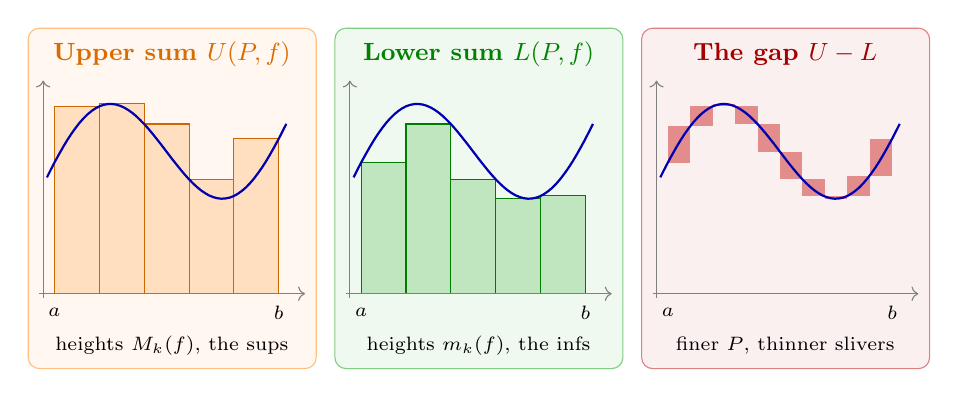
\begin{tikzpicture}[scale=0.95]
% generated: f(x) = 1.0 + 0.3x + 0.75 sin(1.8x) on [0.25, 3.25]
\fill[orange!6,rounded corners] (-0.1,-1.0) rectangle (3.75,3.55);
\draw[orange!50,rounded corners] (-0.1,-1.0) rectangle (3.75,3.55);
\node[font=\small\bfseries,text=orange!85!black] at (1.82,3.2) {Upper sum $U(P,f)$};
\filldraw[fill=orange!25,draw=orange!80!black] (0.250,0) rectangle (0.850,2.505);
\filldraw[fill=orange!25,draw=orange!80!black] (0.850,0) rectangle (1.450,2.538);
\filldraw[fill=orange!25,draw=orange!80!black] (1.450,0) rectangle (2.050,2.269);
\filldraw[fill=orange!25,draw=orange!80!black] (2.050,0) rectangle (2.650,1.530);
\filldraw[fill=orange!25,draw=orange!80!black] (2.650,0) rectangle (3.250,2.075);
\draw[->,gray] (0.05,0) -- (3.6,0);
\draw[->,gray] (0.1,-0.05) -- (0.1,2.85);
\draw[thick,blue!70!black] (0.150,1.556) -- (0.204,1.664) -- (0.258,1.768) -- (0.313,1.868) -- (0.367,1.963) -- (0.421,2.053) -- (0.475,2.136) -- (0.530,2.213) -- (0.584,2.283) -- (0.638,2.344) -- (0.692,2.398) -- (0.747,2.443) -- (0.801,2.480) -- (0.855,2.508) -- (0.909,2.526) -- (0.964,2.536) -- (1.018,2.537) -- (1.072,2.530) -- (1.126,2.514) -- (1.181,2.490) -- (1.235,2.458) -- (1.289,2.420) -- (1.343,2.375) -- (1.397,2.323) -- (1.452,2.267) -- (1.506,2.206) -- (1.560,2.142) -- (1.614,2.074) -- (1.669,2.005) -- (1.723,1.934) -- (1.777,1.863) -- (1.831,1.792) -- (1.886,1.723) -- (1.940,1.656) -- (1.994,1.592) -- (2.048,1.532) -- (2.103,1.476) -- (2.157,1.426) -- (2.211,1.382) -- (2.265,1.345) -- (2.319,1.314) -- (2.374,1.292) -- (2.428,1.277) -- (2.482,1.271) -- (2.536,1.274) -- (2.591,1.285) -- (2.645,1.305) -- (2.699,1.335) -- (2.753,1.373) -- (2.808,1.419) -- (2.862,1.475) -- (2.916,1.538) -- (2.970,1.609) -- (3.025,1.687) -- (3.079,1.771) -- (3.133,1.862) -- (3.187,1.958) -- (3.242,2.059) -- (3.296,2.164) -- (3.350,2.271);
\node[font=\scriptsize] at (0.25,-0.25) {$a$};
\node[font=\scriptsize] at (3.25,-0.25) {$b$};
\node[font=\scriptsize] at (1.82,-0.7) {heights $M_k(f)$, the sups};
\fill[green!60!black!6,rounded corners] (3.9999999999999996,-1.0) rectangle (7.85,3.55);
\draw[green!60!black!50,rounded corners] (3.9999999999999996,-1.0) rectangle (7.85,3.55);
\node[font=\small\bfseries,text=green!60!black!85!black] at (5.92,3.2) {Lower sum $L(P,f)$};
\filldraw[fill=green!60!black!25,draw=green!60!black!80!black] (4.350,0) rectangle (4.950,1.752);
\filldraw[fill=green!60!black!25,draw=green!60!black!80!black] (4.950,0) rectangle (5.550,2.269);
\filldraw[fill=green!60!black!25,draw=green!60!black!80!black] (5.550,0) rectangle (6.150,1.530);
\filldraw[fill=green!60!black!25,draw=green!60!black!80!black] (6.150,0) rectangle (6.750,1.271);
\filldraw[fill=green!60!black!25,draw=green!60!black!80!black] (6.750,0) rectangle (7.350,1.308);
\draw[->,gray] (4.1499999999999995,0) -- (7.699999999999999,0);
\draw[->,gray] (4.199999999999999,-0.05) -- (4.199999999999999,2.85);
\draw[thick,blue!70!black] (4.250,1.556) -- (4.304,1.664) -- (4.358,1.768) -- (4.413,1.868) -- (4.467,1.963) -- (4.521,2.053) -- (4.575,2.136) -- (4.630,2.213) -- (4.684,2.283) -- (4.738,2.344) -- (4.792,2.398) -- (4.847,2.443) -- (4.901,2.480) -- (4.955,2.508) -- (5.009,2.526) -- (5.064,2.536) -- (5.118,2.537) -- (5.172,2.530) -- (5.226,2.514) -- (5.281,2.490) -- (5.335,2.458) -- (5.389,2.420) -- (5.443,2.375) -- (5.497,2.323) -- (5.552,2.267) -- (5.606,2.206) -- (5.660,2.142) -- (5.714,2.074) -- (5.769,2.005) -- (5.823,1.934) -- (5.877,1.863) -- (5.931,1.792) -- (5.986,1.723) -- (6.040,1.656) -- (6.094,1.592) -- (6.148,1.532) -- (6.203,1.476) -- (6.257,1.426) -- (6.311,1.382) -- (6.365,1.345) -- (6.419,1.314) -- (6.474,1.292) -- (6.528,1.277) -- (6.582,1.271) -- (6.636,1.274) -- (6.691,1.285) -- (6.745,1.305) -- (6.799,1.335) -- (6.853,1.373) -- (6.908,1.419) -- (6.962,1.475) -- (7.016,1.538) -- (7.070,1.609) -- (7.125,1.687) -- (7.179,1.771) -- (7.233,1.862) -- (7.287,1.958) -- (7.342,2.059) -- (7.396,2.164) -- (7.450,2.271);
\node[font=\scriptsize] at (4.35,-0.25) {$a$};
\node[font=\scriptsize] at (7.35,-0.25) {$b$};
\node[font=\scriptsize] at (5.92,-0.7) {heights $m_k(f)$, the infs};
\fill[red!75!black!6,rounded corners] (8.1,-1.0) rectangle (11.95,3.55);
\draw[red!75!black!50,rounded corners] (8.1,-1.0) rectangle (11.95,3.55);
\node[font=\small\bfseries,text=red!75!black!85!black] at (10.02,3.2) {The gap $U - L$};
\fill[red!75!black!45] (8.450,1.752) rectangle (8.750,2.240);
\fill[red!75!black!45] (8.750,2.240) rectangle (9.050,2.505);
\fill[red!75!black!45] (9.050,2.504) rectangle (9.350,2.538);
\fill[red!75!black!45] (9.350,2.269) rectangle (9.650,2.504);
\fill[red!75!black!45] (9.650,1.898) rectangle (9.950,2.269);
\fill[red!75!black!45] (9.950,1.530) rectangle (10.250,1.898);
\fill[red!75!black!45] (10.250,1.301) rectangle (10.550,1.530);
\fill[red!75!black!45] (10.550,1.271) rectangle (10.850,1.308);
\fill[red!75!black!45] (10.850,1.308) rectangle (11.150,1.581);
\fill[red!75!black!45] (11.150,1.581) rectangle (11.450,2.075);
\draw[->,gray] (8.25,0) -- (11.799999999999999,0);
\draw[->,gray] (8.299999999999999,-0.05) -- (8.299999999999999,2.85);
\draw[thick,blue!70!black] (8.350,1.556) -- (8.404,1.664) -- (8.458,1.768) -- (8.513,1.868) -- (8.567,1.963) -- (8.621,2.053) -- (8.675,2.136) -- (8.730,2.213) -- (8.784,2.283) -- (8.838,2.344) -- (8.892,2.398) -- (8.947,2.443) -- (9.001,2.480) -- (9.055,2.508) -- (9.109,2.526) -- (9.164,2.536) -- (9.218,2.537) -- (9.272,2.530) -- (9.326,2.514) -- (9.381,2.490) -- (9.435,2.458) -- (9.489,2.420) -- (9.543,2.375) -- (9.597,2.323) -- (9.652,2.267) -- (9.706,2.206) -- (9.760,2.142) -- (9.814,2.074) -- (9.869,2.005) -- (9.923,1.934) -- (9.977,1.863) -- (10.031,1.792) -- (10.086,1.723) -- (10.140,1.656) -- (10.194,1.592) -- (10.248,1.532) -- (10.303,1.476) -- (10.357,1.426) -- (10.411,1.382) -- (10.465,1.345) -- (10.519,1.314) -- (10.574,1.292) -- (10.628,1.277) -- (10.682,1.271) -- (10.736,1.274) -- (10.791,1.285) -- (10.845,1.305) -- (10.899,1.335) -- (10.953,1.373) -- (11.008,1.419) -- (11.062,1.475) -- (11.116,1.538) -- (11.170,1.609) -- (11.225,1.687) -- (11.279,1.771) -- (11.333,1.862) -- (11.387,1.958) -- (11.442,2.059) -- (11.496,2.164) -- (11.550,2.271);
\node[font=\scriptsize] at (8.45,-0.25) {$a$};
\node[font=\scriptsize] at (11.45,-0.25) {$b$};
\node[font=\scriptsize] at (10.02,-0.7) {finer $P$, thinner slivers};
\end{tikzpicture}
\caption{Upper and lower sums for the same partition $P$ of $[a,b]$ into five subintervals. On each subinterval the upper rectangle has height $M_k(f)$ and the lower one height $m_k(f)$, so $L(P,f) \leq \int_a^b f \leq U(P,f)$. The right panel shows the difference $U(P,f) - L(P,f)$ for a refinement into ten subintervals: it is the total area of the slivers, and $f$ is integrable exactly when it can be made as small as we please.}
\label{fig:riemann-sums}
\end{figure}
\end{note}


\begin{thm}\label{thm:refine}
Let $f$ be a bounded function on $[a,b]$.
\begin{enumerate}
\item[(i)] If $P^*$ is a refinement of a partition $P$, then $U(P^*, f)\leq U(P,f)$ and $L(P^*,f)\geq L(P,f)$.
\item[(ii)] For any two partitions $P_1$ and $P_2$, $L(P_1, f)\leq U(P_2,f)$.
\end{enumerate}
\end{thm}

\begin{proof}
(i) Since $P^*$ is obtained from $P$ by adding finitely many points one at a time, it suffices to treat the case where $P^*$ has exactly one more point than $P$, say $c$, lying in the $j^{\text{th}}$ subinterval $(x_{j-1},x_j)$. Let $M'$ and $M''$ be the suprema of $f$ on $[x_{j - 1}, c]$ and $[c,x_j]$. Then $M'\leq M_j(f)$ and $M''\leq M_j(f)$, so
\begin{align*}
U(P^*, f) - U(P,f) &= M'(c - x_{j - 1}) + M''(x_j - c)\\
&\qquad - M_j(f)(x_j - x_{j-1}) \leq 0 .
\end{align*}
The inequality for lower sums is proved in the same way, with infima.

(ii) Let $P = P_1\cup P_2$. By (i),
$$L(P_1,f) \leq L(P,f) \leq U(P,f) \leq U(P_2,f) .$$
\end{proof}

\begin{note}
If $M = \sup \{f(x): x\in [a,b]\}$ and $m = \inf \{f(x): x\in [a,b]\}$, then $m(b-a)\leq L(P_1,f) \leq U(P_2,f)\leq M(b-a)$ for any partitions $P_1$ and $P_2$. In particular the sets of upper sums and of lower sums are bounded.
\end{note}


\begin{defn}
Let $f$ be bounded on $[a,b]$. The \emph{upper Riemann integral} and the \emph{lower Riemann integral} of $f$ over $[a,b]$ are
\begin{align*}
\overline{\int^b_a}f(x)\, dx &= \inf \{U(P,f): P\in \mathcal{P}[a,b]\},\\
\underline{\int^b_a}f(x)\, dx &= \sup \{L(P,f): P\in \mathcal{P}[a,b]\},
\end{align*}
the infimum and supremum being taken over all partitions of $[a,b]$. We shall also write them simply as $\overline{\int^b_a} f$ and $\underline{\int^b_a} f$.
\end{defn}


\begin{thm}
If $f$ is bounded on $[a,b]$, then $\displaystyle\underline{\int^b_a} f \leq \overline{\int^b_a} f$.
\end{thm}

\begin{proof}
By Theorem~\ref{thm:refine}(ii), every lower sum is at most every upper sum. Fix a partition $P_2$: then $U(P_2,f)$ is an upper bound for all lower sums, so $\underline{\int^b_a} f\leq U(P_2,f)$. This holds for every $P_2$, so $\underline{\int^b_a} f$ is a lower bound for all upper sums, and therefore $\underline{\int^b_a} f\leq\overline{\int^b_a} f$.

The inequality can be strict, as the next example shows.
\end{proof}


\begin{exa}
Let $f$ be defined on $[0,1]$ by $f(x) = 1$ if $x$ is rational and $f(x) = 0$ if $x$ is irrational. Every subinterval contains both rational and irrational numbers, so for every partition $P$ of $[0,1]$ we have $M_k(f) = 1$ and $m_k(f) = 0$. Therefore $U(P,f) = 1$ and $L(P,f) = 0$ for all $P$, and
$$\overline{\int^1_0} f = 1 ,\qquad \underline{\int^1_0} f = 0.$$
\end{exa}

\begin{remark}
If $a< c < b$, then
$$\overline{\int^b_a} f = \overline{\int^c_a} f + \overline{\int^b_c} f \qquad\text{and}\qquad \underline{\int^b_a} f = \underline{\int^c_a} f + \underline{\int^b_c} f .$$
However, some properties of upper and lower integrals differ from those of integrals: in general only
$$\overline{\int^b_a} (f + g) \leq \overline{\int^b_a} f + \overline{\int^b_a} g\qquad \text{and}\qquad \underline{\int^b_a} (f + g) \geq \underline{\int^b_a} f + \underline{\int^b_a} g$$
hold, and the inequalities may be strict (take $f$ as in the example and $g = 1-f$).
\end{remark}


\begin{defn}
A bounded function $f$ on $[a,b]$ is said to be \emph{Riemann integrable} on $[a,b]$ if
$$\underline{\int^b_a} f = \overline{\int^b_a} f .$$
The common value is called the \emph{Riemann integral} of $f$ over $[a,b]$ and is denoted by $\int^b_a f$ or $\int^b_a f(x)\,dx$.
\end{defn}


\begin{exa}
Every constant function $f(x) = C$ is Riemann integrable on $[a,b]$, and $\int^b_a C\,dx = C(b-a)$.
\end{exa}

\begin{solution}
For any partition $P$, $M_k(f) = m_k(f) = C$ for every $k$, so
$$U(P,f) = \sum^n_{k = 1} C \Delta x_k = C(b - a) = L(P,f).$$
Hence both the upper and the lower integral equal $C(b-a)$.
\end{solution}


\begin{exa}
Let $f(x)  = x^2$ on $[0,1]$, and for each $n$ let $P_n = \left\{0, \frac{1}{n}, \frac{2}{n}, \dots, \frac{n}{n}\right\}$. Compute $\lim_{n\rightarrow \infty} U(P_n,f)$ and $\lim_{n \rightarrow \infty} L(P_n,f)$, and deduce $\int_0^1x^2\,dx$.
\end{exa}

\begin{solution}
The subintervals of $P_n$ are $\left[\frac{k-1}{n},\frac{k}{n}\right]$, each of length $\frac{1}{n}$. Since $x^2$ is increasing on $[0,1]$,
$$M_k(f) = \left(\frac{k}{n}\right)^2,\qquad m_k (f) = \left(\frac{k - 1}{n}\right)^2 .$$
Using $1^2 + 2^2 + \dots + n^2 = \frac{n(n + 1)(2n + 1)}{6}$,
$$U(P_n,f) = \frac{1}{n^3}\sum^n_{k = 1}k^2 = \frac{(n + 1)(2n + 1)}{6n^2}\longrightarrow\frac{2}{6} = \frac{1}{3},$$
$$L(P_n,f) = \frac{1}{n^3}\sum^n_{k = 1}(k-1)^2 = \frac{(n - 1)(2n - 1)}{6n^2} \longrightarrow \frac{1}{3} .$$
Since $L(P_n, f) \leq \underline{\int^1_0} f \leq \overline{\int^1_0} f \leq U(P_n, f)$ and both bounds tend to $\frac{1}{3}$, $f$ is integrable and $\int^1_0 x^2\, dx = \frac{1}{3}$.
\end{solution}


\begin{thm}[Riemann's Criterion]\label{thm:riemanncrit}
A bounded function $f$ on $[a,b]$ is Riemann integrable if and only if for every $\varepsilon >0$ there is a partition $P$ of $[a,b]$ such that $U(P, f) - L(P,f) < \varepsilon$.
\end{thm}

\begin{proof}
We have already seen that
\begin{equation}\label{eq:lowup}
\underline{\int^b_a} f \leq \overline{\int^b_a} f .
\end{equation}
Suppose that for every $\varepsilon > 0$ there is a partition $P$ with $U(P,f) - L(P, f) < \varepsilon$. Since $\overline{\int^b_a} f \leq U(P,f)$ and $\underline{\int^b_a} f \geq L(P,f)$,
$$\overline{\int^b_a}f - \underline{\int^b_a}f \leq U(P,f) - L(P,f) < \varepsilon .$$
Since $\varepsilon  > 0$ is arbitrary,
\begin{equation}\label{eq:uplow}
\overline{\int^b_a}f \leq \underline{\int^b_a}f ,
\end{equation}
and \eqref{eq:lowup} and \eqref{eq:uplow} together show that $f$ is Riemann integrable.

Conversely, suppose that $f$ is Riemann integrable, with integral $I$, and let $\varepsilon >  0$. By the definitions of infimum and supremum there are partitions $P_1$ and $P_2$ with
$$U(P_1,f) < I + \frac{\varepsilon}{2} \qquad\text{and}\qquad L(P_2,f) > I - \frac{\varepsilon}{2}.$$
Let $P = P_1\cup P_2$. By Theorem~\ref{thm:refine}, $U(P,f)\leq U(P_1,f)$ and $L(P,f)\geq L(P_2,f)$, so
$$U(P,f) - L(P,f) < \left(I + \frac{\varepsilon}{2}\right) - \left(I - \frac{\varepsilon}{2}\right) = \varepsilon .$$
\end{proof}


\begin{thm}\label{thm:contint}
Every continuous function on $[a,b]$ is Riemann integrable. More precisely, for every $\varepsilon>0$ there is a $\delta>0$ such that $U(P,f) - L(P,f)<\varepsilon$ for every partition $P$ with $\|P\|<\delta$.
\end{thm}

\begin{proof}
Let $f$ be continuous on $[a,b]$ and $\varepsilon > 0$. Since $f$ is uniformly continuous on $[a,b]$, there is a $\delta > 0$ such that $|f(x) - f(y)| < \frac{\varepsilon}{b - a}$ whenever $x, y\in [a,b]$ and $|x - y| < \delta$.

Let $P$ be any partition with $\|P\| < \delta$. On each closed subinterval $[x_{k-1},x_k]$ the continuous function $f$ attains its maximum and minimum, say $M_k = f(x_k')$ and $m_k = f(x_k'')$. Since $|x_k' - x_k''|\leq\Delta x_k < \delta$, we get $M_k - m_k < \frac{\varepsilon}{b - a}$, and so
$$U(P,f) - L(P,f) = \sum^n_{k = 1}(M_k - m_k)\Delta x_k < \frac{\varepsilon}{b - a}\sum^n_{k = 1}\Delta x_k = \varepsilon .$$
By Riemann's Criterion, $f$ is Riemann integrable.
\end{proof}


\begin{thm}
Every monotone function on $[a,b]$ is Riemann integrable.
\end{thm}

\begin{proof}
Suppose $f$ is increasing. If $f(a) = f(b)$, then $f$ is constant and integrable. Otherwise $f(a)<f(b)$. Let $\varepsilon > 0$, and let $P$ be any partition with $\|P\| < \frac{\varepsilon}{f(b) - f(a)}$. Since $f$ is increasing, $M_k(f) =f(x_k)$ and $m_k(f) = f(x_{k-1})$ on $[x_{k - 1}, x_k]$. Hence
\begin{align*}
U(P,f) - L(P,f) &= \sum^n_{k  = 1} \bigl(f(x_k) - f(x_{k - 1})\bigr) \Delta x_k\\
&< \frac{\varepsilon}{f(b) - f(a)} \sum^n_{k  = 1} \bigl(f(x_k) - f(x_{k - 1})\bigr) = \varepsilon ,
\end{align*}
since the last sum telescopes to $f(b)-f(a)$. By Riemann's Criterion, $f$ is integrable. If $f$ is decreasing, apply this to $-f$ and use Theorem~\ref{thm:cf} below, or repeat the argument with $M_k(f) = f(x_{k-1})$ and $m_k(f) = f(x_k)$.
\end{proof}


\begin{exa}
Let $f$ be continuous on $[0,1]$, let $\sigma_n = \left\{0, \frac{1}{n}, \frac{2}{n}, \dots, \frac{n}{n}\right\}$, and let $x^*_k$ be any point of $\left[\frac{k - 1}{n}, \frac{k}{n}\right]$.
\begin{enumerate}
\item[(i)] Prove that $L(\sigma_n, f) \leq \frac{1}{n} \sum_{k =1}^n f(x^*_k) \leq U(\sigma_n,f)$.
\item[(ii)] Hence show that $\lim_{n\rightarrow\infty}\frac{1}{n} \sum^n_{k  = 1} f(x^*_k) = \int^1_0f(x)\, dx$.
\end{enumerate}
\end{exa}

\begin{solution}
(i) Here $\Delta x_k = \frac{1}{n}$, so $\frac{1}{n}\sum_{k=1}^n f(x_k^*)$ is a Riemann sum for $\sigma_n$, and it lies between $L(\sigma_n,f)$ and $U(\sigma_n,f)$ because $m_k(f)\leq f(x^*_k)\leq M_k(f)$.

(ii) Let $I = \int_0^1 f$, which exists by Theorem~\ref{thm:contint}. We also have $L(\sigma_n,f)\leq I\leq U(\sigma_n,f)$. Let $\varepsilon>0$ and choose $\delta$ as in Theorem~\ref{thm:contint}. For $n>\frac{1}{\delta}$, $\|\sigma_n\| = \frac{1}{n}<\delta$, so $U(\sigma_n,f) - L(\sigma_n,f)<\varepsilon$. Both $I$ and the Riemann sum lie in the interval $[L(\sigma_n,f), U(\sigma_n,f)]$, whose length is less than $\varepsilon$, so
$$\left|\frac{1}{n}\sum_{k=1}^n f(x^*_k) - I\right|<\varepsilon \qquad\text{for } n>\tfrac{1}{\delta}.$$
\end{solution}


\begin{exa}
Let $f(x) = \frac{\sin x}{x}$ for $0<x\leq1$ and $f(0) = 1$. Prove that $f$ is Riemann integrable on $[0,1]$.
\end{exa}

\begin{solution}
The function $\frac{\sin x}{x}$ is continuous for $x\neq 0$, and its limit at $0$ is $1 = f(0)$. So $f$ is continuous on $[0,1]$, and Theorem~\ref{thm:contint} shows that it is Riemann integrable.
\end{solution}


\begin{exa}
\begin{enumerate}
\item[(i)] The function $f$ on $[0,1]$ with $f(x) = 1$ for rational $x$ and $f(x) = 0$ for irrational $x$ is bounded but not Riemann integrable, since its upper and lower integrals are $1$ and $0$.

\item[(ii)] A discontinuous function may be integrable. Let $f(x) = 1$ for $x\in \left[0, \frac{1}{2}\right]$ and $f(x) = 0$ for $x\in \left(\frac{1}{2}, 1\right]$. Then $f$ is discontinuous at $\frac{1}{2}$. Let $P$ be any partition of $[0,1]$, and let $k$ be the index with $x_{k-1}\leq\frac{1}{2}<x_k$. On the subintervals before the $k^{\text{th}}$, $M_i = m_i = 1$; on those after it, $M_i = m_i = 0$; and on $[x_{k-1},x_k]$, which contains $\frac{1}{2}$ and points beyond it, $M_k = 1$ and $m_k = 0$. Hence
$$U(P,f) = x_k\qquad\text{and}\qquad L(P,f) = x_{k-1},$$
so $L(P,f)\leq\frac{1}{2}<U(P,f)$ and $U(P,f) - L(P,f) = \Delta x_k\leq\|P\|$. Taking partitions with small norm, Riemann's Criterion (Theorem~\ref{thm:riemanncrit}) shows that $f$ is integrable, and since $\frac{1}{2}$ lies between every lower and every upper sum, $\int^1_0 f = \frac{1}{2}$, the length of the interval on which $f = 1$.
\end{enumerate}
\end{exa}


\begin{thm}
A bounded function $f$ on $[a,b]$ is Riemann integrable if
\begin{enumerate}
\item[(i)] it has only finitely many points of discontinuity in $[a,b]$, or
\item[(ii)] its set of points of discontinuity has only finitely many limit points.
\end{enumerate}
\end{thm}

\begin{proof}
Let $M = \sup f$ and $m = \inf f$ on $[a,b]$. If $M = m$, $f$ is constant; so assume $M>m$. Let $\varepsilon>0$.

(i) Let $\alpha_1<\alpha_2<\dots<\alpha_p$ be the points of discontinuity. Enclose them in non-overlapping intervals $[x_1', x''_1], \dots, [x_p',x_p'']$, each containing its point $\alpha_r$ in its interior (or as an end point if $\alpha_r = a$ or $b$), with total length
$$\sum^p_{r = 1}(x''_r - x'_r) < \frac{\varepsilon}{2(M - m)} .$$
On each of the $p + 1$ remaining closed intervals $[a,x_1'], [x''_1,x'_2], \dots, [x''_p,b]$ the function $f$ is continuous, hence integrable, so by Riemann's Criterion there are partitions $P_1, \dots, P_{p+1}$ of them with
$$U(P_r,f) - L(P_r,f) < \frac{\varepsilon}{2(p+1)}, \qquad r =1, 2, \dots, p + 1 .$$
Let $P$ be the partition of $[a,b]$ formed by all the points of $P_1,\dots,P_{p+1}$. Its subintervals are those of the $P_r$ together with the intervals $[x'_r,x''_r]$, on which the oscillation $M'_r - m'_r$ is at most $M - m$. Hence
\begin{align*}
U(P,f) - L(P,f) &\leq (M-m)\sum^p_{r=1}(x''_r-x'_r) + \sum^{p + 1}_{r=1}\bigl(U(P_r,f) - L(P_r,f)\bigr)\\
&< \frac{\varepsilon}{2} + \frac{\varepsilon}{2} = \varepsilon,
\end{align*}
and $f$ is integrable by Riemann's Criterion.

(ii) Let $\alpha_1,\dots,\alpha_p$ be the limit points of the set $D$ of discontinuities, and enclose them as in (i) in intervals of total length less than $\frac{\varepsilon}{2(M-m)}$. Each of the remaining closed intervals contains only finitely many points of $D$: otherwise, by the Bolzano--Weierstrass Theorem, $D$ would have a limit point in that closed interval, but all limit points of $D$ lie in the enclosing intervals' interiors. By part (i), $f$ is integrable on each remaining interval, and the argument of (i) gives a partition $P$ with $U(P,f) - L(P,f) < \varepsilon$.
\end{proof}

\begin{exa}
Using upper and lower sums, show that $\int_0^b x\,dx = \frac{b^2}{2}$ for $b>0$.
\end{exa}

\begin{solution}
Let $P_n$ divide $[0,b]$ into $n$ equal parts, $x_k = \frac{kb}{n}$. Since $f(x) = x$ is increasing, $M_k = \frac{kb}{n}$ and $m_k = \frac{(k-1)b}{n}$, so with $\Delta x_k = \frac{b}{n}$,
$$U(P_n,f) = \frac{b^2}{n^2}\sum_{k=1}^nk = \frac{b^2}{n^2}\cdot\frac{n(n+1)}{2} = \frac{b^2}{2}\left(1+\frac{1}{n}\right),\qquad L(P_n,f) = \frac{b^2}{2}\left(1-\frac{1}{n}\right).$$
Both tend to $\frac{b^2}{2}$, and $U(P_n,f) - L(P_n,f) = \frac{b^2}{n}\longrightarrow 0$. By Riemann's Criterion $f$ is integrable, and its integral lies between $L(P_n,f)$ and $U(P_n,f)$ for every $n$, so it equals $\frac{b^2}{2}$.
\end{solution}

\begin{exa}
Compute the midpoint Riemann sum of $f(x) = \frac{1}{1+x^2}$ on $[0,1]$ with $n = 4$, and compare it with $\int_0^1\frac{dx}{1+x^2} = \frac{\pi}{4}$.
\end{exa}

\begin{solution}
The midpoints of the four subintervals are $\frac{1}{8}, \frac{3}{8}, \frac{5}{8}, \frac{7}{8}$, where $f$ takes the values
$$0.984615,\qquad 0.876712,\qquad 0.719101,\qquad 0.566372 .$$
The Riemann sum is $\frac{1}{4}(0.984615 + 0.876712 + 0.719101 + 0.566372) = 0.786700$, while $\frac{\pi}{4} = 0.785398$. Four evaluations already give $\pi\approx 4\times0.7867 = 3.1468$. Since $f$ is decreasing on $[0,1]$, the upper and lower sums for this partition are guaranteed bounds: $L = \frac{1}{4}\bigl(f(\frac14)+f(\frac12)+f(\frac34)+f(1)\bigr)\approx 0.7203$ and $U = L + \frac{1}{4}\bigl(f(0) - f(1)\bigr)\approx 0.8453$, so $0.7203<\frac{\pi}{4}<0.8453$.
\end{solution}

\begin{exa}[Thomae's function is integrable]
Let $f$ be Thomae's function on $[0,1]$: $f(x) = \frac{1}{q}$ if $x = \frac{p}{q}$ in lowest terms, and $f(x) = 0$ if $x$ is irrational (with $f(0) = f(1) = 1$). Show that $f\in R[0,1]$ and $\int_0^1f = 0$, although $f$ is discontinuous at every rational point.
\end{exa}

\begin{solution}
Every subinterval contains irrational points, so $m_k = 0$ and $L(P,f) = 0$ for every partition. It remains to make $U(P,f)$ small. Let $\varepsilon>0$ and choose $N$ with $\frac{1}{N}<\frac{\varepsilon}{2}$. Only finitely many points of $[0,1]$, say $K$ of them, have $f(x)\geq\frac{1}{N}$ (the rationals with denominator at most $N$). Choose a partition $P$ in which each of these $K$ points lies in subintervals of total length less than $\frac{\varepsilon}{2}$ (at most two subintervals per point). On those subintervals $M_k\leq 1$; on all the others $M_k<\frac{1}{N}$. Hence
$$U(P,f) < 1\cdot\frac{\varepsilon}{2} + \frac{1}{N}\cdot 1<\varepsilon .$$
By Riemann's Criterion $f$ is integrable, and $0 = L(P,f)\leq\int_0^1f\leq U(P,f)<\varepsilon$ for every $\varepsilon$, so $\int_0^1 f = 0$. This function has infinitely many discontinuities, with every point of $[0,1]$ a limit point of them, so the last theorem does not apply; yet it is integrable.
\end{solution}


\subsection{Properties of the Riemann Integral}

We now establish the basic properties of the integral. We denote the set of all Riemann integrable functions on $[a,b]$ by $R[a,b]$, and write $f\in R[a,b]$ to mean that $f$ is Riemann integrable on $[a,b]$.


\begin{thm}\label{thm:cf}
If $f\in R[a,b]$ and $C$ is any real number, then $Cf\in R[a,b]$ and
$$\int^b_aCf = C\int^b_af.$$
\end{thm}

\begin{proof}
If $C\geq 0$, then $M_k(Cf) = CM_k(f)$ and $m_k(Cf) = Cm_k(f)$ on every subinterval, so $U(P,Cf) = CU(P,f)$ and $L(P,Cf) = CL(P,f)$ for every partition $P$. Taking the infimum and supremum over $P$,
$$\overline{\int^b_a}Cf = C\,\overline{\int^b_a}f = C\int^b_af = C\,\underline{\int^b_a}f = \underline{\int^b_a}Cf .$$

If $C<0$, multiplying by $C$ reverses inequalities, so $M_k(Cf) = Cm_k(f)$ and $m_k(Cf) = CM_k(f)$. Hence $U(P,Cf) = CL(P,f)$ and $L(P,Cf) = CU(P,f)$, and
\begin{align*}
\overline{\int^b_a}Cf &= \inf_P C L(P,f) = C\sup_P L(P,f) = C\int^b_a f,\\
\underline{\int^b_a}Cf &= \sup_P CU(P,f) = C\inf_P U(P,f) = C\int^b_a f .
\end{align*}
In both cases $Cf\in R[a,b]$ and $\int_a^b Cf = C\int_a^b f$.
\end{proof}


\begin{thm}
Let $c\in [a,b]$. Then $f\in R[a,b]$ if and only if $f\in R[a,c]$ and $f\in R[c,b]$. In this case
$$\int^b_af = \int^c_af + \int^b_cf.$$
\end{thm}

\begin{proof}
If $c = a$ or $c = b$ there is nothing to prove, so let $a<c<b$. Partitions $P_1$ of $[a,c]$ and $P_2$ of $[c,b]$ combine into a partition $P_1\cup P_2$ of $[a,b]$, with
\begin{align*}
U(P_1\cup P_2, f) &= U(P_1,f) + U(P_2,f),\\
L(P_1\cup P_2, f) &= L(P_1,f) + L(P_2,f).
\end{align*}

Suppose $f\in R[a,b]$ and $\varepsilon>0$. By Riemann's Criterion there is a partition $P$ of $[a,b]$ with $U(P,f) - L(P,f) < \varepsilon$, and by Theorem~\ref{thm:refine} the refinement $P^* = P\cup\{c\}$ satisfies the same inequality. Splitting $P^*$ at $c$ into $P_1$ and $P_2$,
\begin{align*}
&\bigl(U(P_1,f) - L(P_1,f)\bigr) + \bigl(U(P_2,f) - L(P_2,f)\bigr)\\
&\qquad = U(P^*,f) - L(P^*,f) < \varepsilon .
\end{align*}
Both brackets are non-negative, so each is less than $\varepsilon$, and $f\in R[a,c]$, $f\in R[c,b]$.

Conversely, if $f\in R[a,c]$ and $f\in R[c,b]$, choose $P_1$ and $P_2$ with $U(P_i,f) - L(P_i,f) < \frac{\varepsilon}{2}$; then $P = P_1\cup P_2$ gives $U(P,f) - L(P,f) <\varepsilon$, so $f\in R[a,b]$.

Finally, for any such $P_1$ and $P_2$,
$$L(P_1,f) + L(P_2,f) \leq \int_a^b f\leq U(P_1,f) + U(P_2,f).$$
Taking the supremum of the left side and the infimum of the right side over $P_1$ and $P_2$ gives $\int_a^c f + \int_c^b f\leq\int_a^b f\leq\int_a^c f + \int_c^b f$.
\end{proof}

\begin{note}
We define $\int_a^a f = 0$ and $\int_b^a f = -\int_a^b f$ for $a<b$. With these conventions the formula $\int^b_af = \int^c_af + \int^b_cf$ holds for any $a,b,c$ in an interval on which $f$ is integrable, whatever their order.
\end{note}


\begin{coro}
If $f\in R[a,b]$ and $[c,d]\subseteq [a,b]$, then $f\in R[c,d]$. That is, a function integrable on a closed bounded interval is integrable on every closed subinterval.
\end{coro}

\begin{proof}
Apply the theorem twice: $f\in R[a,b]$ gives $f\in R[c,b]$, and then $f\in R[c,d]$.
\end{proof}


\begin{thm}
If $f, g\in R[a,b]$, then $f + g\in R[a,b]$ and
$$\int^b_a(f  + g) = \int^b_af + \int^b_ag .$$
\end{thm}

\begin{proof}
On any subinterval, $f(x) + g(x)\leq M_k(f) + M_k(g)$, so $M_k(f+g)\leq M_k(f) + M_k(g)$; similarly $m_k(f+g)\geq m_k(f) + m_k(g)$. Hence for every partition $P$,
$$L(P,f) + L(P,g)\leq L(P,f+g)\leq U(P,f+g)\leq U(P,f) + U(P,g).$$
Given $\varepsilon>0$, choose (by Riemann's Criterion and a common refinement) a partition $P$ with $U(P,f) - L(P,f)<\frac{\varepsilon}{2}$ and $U(P,g) - L(P,g)<\frac{\varepsilon}{2}$. Then $U(P,f+g) - L(P,f+g)<\varepsilon$, so $f+g\in R[a,b]$. Moreover both $\int_a^b(f+g)$ and $\int_a^bf + \int_a^bg$ lie between $L(P,f) + L(P,g)$ and $U(P,f) + U(P,g)$, which differ by less than $\varepsilon$. Since $\varepsilon$ is arbitrary, the two numbers are equal.
\end{proof}


\begin{thm}
Let $f,g\in R[a,b]$ with $f\leq g$ on $[a,b]$. Then $\displaystyle\int^b_a f\leq \int^b_ag$.
\end{thm}

\begin{proof}
For every partition $P$, $m_k(f)\leq m_k(g)$ on each subinterval, so $L(P,f)\leq L(P,g)\leq\int_a^bg$. Taking the supremum over $P$ gives $\int_a^b f\leq\int_a^bg$.
\end{proof}


\begin{thm}\label{thm:productint}
If $f, g\in R[a,b]$, then $fg\in R[a,b]$.
\end{thm}

\begin{proof}
Since $f$ and $g$ are bounded, there is a $K> 0$ with $|f|\leq K$ and $|g|\leq K$ on $[a,b]$; then $|fg|\leq K^2$, so $fg$ is bounded. Let $\varepsilon>0$, and choose a partition $P$ with $U(P,f) - L(P,f) <\varepsilon$ and $U(P,g) - L(P,g)<\varepsilon$. For $x', x''$ in a subinterval $[x_{r - 1}, x_r]$,
\begin{align*}
&|f(x'')g(x'') - f(x')g(x')|\\
&\qquad = \bigl|g(x'')\bigl(f(x'') - f(x')\bigr) + f(x')\bigl(g(x'') - g(x')\bigr)\bigr|\\
&\qquad \leq K \bigl(M_r(f) - m_r(f)\bigr) + K \bigl(M_r(g) - m_r(g)\bigr) .
\end{align*}
Taking the supremum over $x'$ and $x''$, $M_r(fg) - m_r(fg)\leq K(M_r(f) - m_r(f)) + K(M_r(g) - m_r(g))$. Multiplying by $\Delta x_r$ and summing,
\begin{align*}
U(P,fg) - L(P,fg) &\leq K\bigl(U(P,f) - L(P,f)\bigr) + K\bigl(U(P,g) - L(P,g)\bigr)\\
&< 2K\varepsilon .
\end{align*}
Since $\varepsilon$ is arbitrary, $fg\in R[a,b]$ by Riemann's Criterion.
\end{proof}


\begin{thm}
Let $f, g\in R[a,b]$, and suppose there is a $t>0$ with $|g| \geq t$ on $[a,b]$. Then $\frac{f}{g}\in R[a,b]$.
\end{thm}

\begin{proof}
For $x',x''$ in a subinterval $[x_{r-1},x_r]$,
$$\left|\frac{1}{g(x'')} - \frac{1}{g(x')}\right| = \frac{|g(x') - g(x'')|}{|g(x')|\,|g(x'')|}\leq\frac{M_r(g) - m_r(g)}{t^2},$$
so $U\left(P,\frac{1}{g}\right) - L\left(P,\frac{1}{g}\right)\leq\frac{1}{t^2}\bigl(U(P,g) - L(P,g)\bigr)$. By Riemann's Criterion $\frac{1}{g}\in R[a,b]$, and then $\frac{f}{g} = f\cdot\frac{1}{g}\in R[a,b]$ by Theorem~\ref{thm:productint}.
\end{proof}


\begin{thm}
If $f\in R[a,b]$ then $|f| \in R[a,b]$ and $\displaystyle\left|\int^b_a f\right| \leq \int^b_a|f|$.
\end{thm}

\begin{proof}
For $x',x''$ in a subinterval, $\bigl||f(x'')| - |f(x')|\bigr|\leq|f(x'') - f(x')|$, so $M_r(|f|) - m_r(|f|) \leq M_r(f) - m_r(f)$. Hence
$$U(P,|f|) - L(P,|f|)\leq U(P,f) - L(P,f)$$
for every $P$, and $|f|\in R[a,b]$ by Riemann's Criterion. Since $-|f|\leq f\leq|f|$, the previous theorems give $-\int_a^b|f|\leq\int_a^bf\leq\int_a^b|f|$, that is, $\left|\int^b_a f\right| \leq \int^b_a|f|$.
\end{proof}

\begin{note}
If $f\in R[a,b]$ and $m\leq f\leq M$ on $[a,b]$, then
$$m(b - a)\leq \int^b_af \leq M(b-a),$$
by the monotonicity of the integral applied to the constants $m$ and $M$.
\end{note}


\begin{thm}[Mean Value Theorem of Integrals]
If $f$ is continuous on $[a,b]$, then there is a number $c$ with $a \leq c \leq b$ such that
$$\int^b_a f(x)\,dx = (b-a) f(c) .$$
\end{thm}

\begin{proof}
Let $m$ and $M$ be the minimum and maximum of $f$ on $[a,b]$. By the note above,
$$m\leq \frac{1}{b - a} \int^b_af(x)\, dx \leq M .$$
By the Intermediate Value Theorem, the continuous function $f$ takes every value between its minimum and its maximum, so $f(c) = \frac{1}{b - a}\int^b_a f(x) \,dx$ for some $c\in[a,b]$.
\end{proof}


\begin{thm}[Generalized Mean Value Theorem for Integrals]
If $f$ and $g$ are continuous on $[a,b]$ and $g(x)\geq 0$ for all $x\in [a,b]$, then there is a point $c\in [a,b]$ such that
$$\int^b_af(x) g(x) \, dx = f(c) \int^b_ag(x)\, dx .$$
\end{thm}

\begin{proof}
Let $m$ and $M$ be the minimum and maximum of $f$ on $[a,b]$. Since $g\geq 0$, $m g(x) \leq f(x) g(x) \leq M g(x)$ on $[a,b]$, and integrating,
$$m \int^b_ag \leq \int^b_afg \leq M \int^b_ag .$$
If $\int_a^bg = 0$, then $\int_a^bfg = 0$ and any $c$ will do. Otherwise $\int_a^bg>0$, and $\mu = \frac{\int_a^bfg}{\int_a^bg}$ lies in $[m,M]$; by the Intermediate Value Theorem $f(c) = \mu$ for some $c\in [a,b]$.
\end{proof}


\begin{exa}
Find a point $c\in[0,1]$ such that $\displaystyle\int^1_0 \frac{x}{1 + x^2}\,dx = c\int_0^1\frac{1}{1+x^2}\,dx$.
\end{exa}

\begin{solution}
Apply the Generalized Mean Value Theorem with $f(x) = x$ and $g(x) = \frac{1}{1 + x^2}\geq0$: a point $c\in[0,1]$ with the stated property exists. To find it, compute both integrals (using the Fundamental Theorem of Calculus, proved in the next section):
$$\int^1_0\frac{1}{1 + x^2} dx = \tan^{-1}(1) - \tan^{-1}(0) = \frac{\pi}{4},\qquad \int^1_0\frac{x}{1 + x^2} dx = \frac{1}{2}\ln (1 + x^2)\Big|^1_0 = \frac{1}{2}\ln 2 .$$
Thus $\frac{1}{2}\ln 2 = \frac{\pi}{4} c$, and $c = \frac{2\ln 2}{\pi}\approx 0.441$.
\end{solution}

\begin{exa}
Without evaluating the integrals, show that
$$\frac{1}{\sqrt{2}}\leq\int_0^1\frac{dx}{\sqrt{1+x^4}}\leq 1 \qquad\text{and}\qquad 1\leq\int_0^1e^{x^2}\,dx\leq e .$$
\end{exa}

\begin{solution}
On $[0,1]$, $1\leq 1+x^4\leq 2$, so $\frac{1}{\sqrt{2}}\leq\frac{1}{\sqrt{1+x^4}}\leq 1$. Since the length of the interval is $1$, the note on bounds gives the first pair of inequalities. (The integral is about $0.927$.) Similarly $1\leq e^{x^2}\leq e$ on $[0,1]$. A sharper upper bound comes from $x^2\leq x$ on $[0,1]$: $\int_0^1e^{x^2}dx\leq\int_0^1e^x\,dx = e - 1\approx 1.718$.
\end{solution}

\begin{exa}
Find the average value of $f(x) = x^2$ on $[0,3]$ and a point $c$ where $f$ attains it, as predicted by the Mean Value Theorem of Integrals.
\end{exa}

\begin{solution}
$\int_0^3x^2\,dx = \frac{x^3}{3}\Big|_0^3 = 9$, so the average value is $\frac{1}{3-0}\cdot 9 = 3$. Solving $c^2 = 3$ in $[0,3]$ gives $c = \sqrt{3}\approx 1.732$.
\end{solution}

\begin{exa}
Show that the converse of the theorem on $|f|$ is false: $|f|$ may be integrable when $f$ is not.
\end{exa}

\begin{solution}
Let $f(x) = 1$ for rational $x$ and $f(x) = -1$ for irrational $x$, on $[0,1]$. Then $|f| = 1$ is integrable. But every subinterval contains both kinds of points, so $U(P,f) = 1$ and $L(P,f) = -1$ for every partition, and $f$ is not integrable.
\end{solution}

\begin{exa}
Show that $\left|\int_0^{2\pi}\sin x\,dx\right|<\int_0^{2\pi}|\sin x|\,dx$, and compute both sides.
\end{exa}

\begin{solution}
$\int_0^{2\pi}\sin x\,dx = -\cos x\Big|_0^{2\pi} = 0$. On $[0,\pi]$, $|\sin x| = \sin x$, and on $[\pi,2\pi]$, $|\sin x| = -\sin x$, so by additivity
$$\int_0^{2\pi}|\sin x|\,dx = \int_0^\pi\sin x\,dx - \int_\pi^{2\pi}\sin x\,dx = 2 - (-2) = 4 .$$
The inequality $|\int f|\leq\int|f|$ is strict here because $f$ changes sign: positive and negative parts cancel in $\int f$ but not in $\int|f|$.
\end{solution}


\subsection{Fundamental Theorem of Calculus}

We now show that every continuous function on $[a,b]$ is the derivative of its integral. If $f\in R[a,b]$, then $f\in R[a,x]$ for every $x\in [a,b]$, so the function
$$F(x) = \int^x_af(t)\, dt,\qquad x\in [a,b],$$
is well defined. It is called the \emph{indefinite integral} of $f$.


\begin{thm}
Let $f\in R[a,b]$ and $F(x) = \int^x_af(t)\, dt$ for $x\in [a,b]$. Then $F$ is continuous on $[a,b]$. If $f$ is continuous at a point $c\in [a,b]$, then $F$ is differentiable at $c$ and $F'(c) = f(c)$.
\end{thm}

\begin{proof}
\emph{Continuity.} Let $M$ be a bound for $|f|$ on $[a,b]$. If $x, x + h\in [a,b]$, then
$$|F(x  + h) - F(x)| = \left|\int^{x + h}_xf(t)\, dt\right| \leq M |h| .$$
So $F$ is Lipschitz, and in particular continuous, on $[a,b]$.

\emph{Differentiability.} Let $f$ be continuous at $c$ and $\varepsilon > 0$. There is a $\delta > 0$ such that $|f(t) - f(c)| < \varepsilon$ whenever $t\in[a,b]$ and $|t - c| < \delta$. If $0<|h|<\delta$ and $c+h\in[a,b]$, then, since $\frac{1}{h}\int_c^{c+h} f(c)\,dt = f(c)$,
$$\left|\frac{F(c + h) - F(c)}{h} - f(c)\right| = \left|\frac{1}{h} \int^{c+h}_c\bigl(f(t) - f(c)\bigr) dt\right| \leq \frac{1}{|h|}\cdot|h|\,\varepsilon = \varepsilon .$$
Hence $F'(c) = f(c)$ (a one-sided derivative if $c$ is an end point).
\end{proof}


\begin{thm}[First Fundamental Theorem of Calculus]
If $f$ is continuous on $[a,b]$ and $F(x) = \int^x_af(t)\, dt$, then $F'(x) = f(x)$ for every $x\in [a,b]$.
\end{thm}

\begin{proof}
This follows from the previous theorem, since $f$ is continuous at every point. Here is a second proof, using the Mean Value Theorem of Integrals. Let $x\in[a,b]$ and $h\neq0$ with $x+h\in[a,b]$. By that theorem,
\begin{equation}\label{eq:ftcquot}
\frac{F(x + h) - F(x)}{h} = \frac{1}{h}\int_x^{x+h}f(t)\,dt = f(C(h))
\end{equation}
for some $C(h)$ between $x$ and $x+h$. As $h\longrightarrow0$, $C(h)\longrightarrow x$, and since $f$ is continuous at $x$, the right side of \eqref{eq:ftcquot} tends to $f(x)$. Hence $F'(x) = f(x)$.
\end{proof}


\begin{thm}[Second Fundamental Theorem of Calculus]
If $f$ is continuous on $[a,b]$ and $\Phi$ is a function on $[a,b]$ with $\Phi' (x) = f(x)$ for every $x\in [a,b]$, then
$$\int^b_af(x)\, dx = \Phi (b) - \Phi (a) .$$
\end{thm}

\begin{proof}
Let $F(x) = \int^{x}_a f(t)\, dt$. By the First Fundamental Theorem, $F' = f = \Phi'$ on $[a,b]$, so $(F-\Phi)' = 0$, and $F - \Phi$ is constant on $[a,b]$ (by the Mean Value Theorem). Hence
$$\int_a^bf = F(b) - F(a) = \Phi(b) - \Phi(a),$$
since $F(a) = 0$. We write $\Phi(b) - \Phi(a) = \Phi(x)\big|_a^b$.
\end{proof}

\begin{exa}
Find $\displaystyle\frac{d}{dx}\int_0^{x^2}\sin(t^2)\,dt$ and $\displaystyle\frac{d}{dx}\int_x^{3x}\frac{dt}{t}$ for $x>0$.
\end{exa}

\begin{solution}
Let $F(u) = \int_0^u\sin(t^2)\,dt$, so that $F'(u) = \sin(u^2)$. The first function is $F(x^2)$, and by the Chain Rule its derivative is $F'(x^2)\cdot 2x = 2x\sin(x^4)$.

For the second, with $G(u) = \int_1^u\frac{dt}{t}$, the function is $G(3x) - G(x)$, with derivative $\frac{3}{3x} - \frac{1}{x} = 0$. So $\int_x^{3x}\frac{dt}{t}$ is constant, equal to its value $\ln 3$ (in agreement with $\ln 3x - \ln x = \ln 3$).
\end{solution}

\begin{exa}
Evaluate $\displaystyle\lim_{x\rightarrow 0}\frac{1}{x}\int_0^x\cos(t^2)\,dt$.
\end{exa}

\begin{solution}
Let $F(x) = \int_0^x\cos(t^2)\,dt$. Then $F(0) = 0$, and by the Fundamental Theorem $F'(0) = \cos 0 = 1$. The limit is $\lim_{x\rightarrow0}\frac{F(x) - F(0)}{x - 0} = F'(0) = 1$. No antiderivative of $\cos(t^2)$ in elementary terms is needed.
\end{solution}

\begin{exa}
Let $f = \operatorname{sgn}$ on $[-1,1]$ (equal to $-1$, $0$, $1$ for $x<0$, $x=0$, $x>0$) and $F(x) = \int_{-1}^xf(t)\,dt$. Find $F$, and show that $F$ is continuous everywhere but not differentiable at $0$.
\end{exa}

\begin{solution}
The function $f$ is integrable, having one discontinuity. For $x\leq0$, $F(x) = \int_{-1}^x(-1)\,dt = -(x+1)$; for $x\geq 0$, $F(x) = -1 + \int_0^x 1\,dt = x - 1$. So $F(x) = |x| - 1$. This is continuous, as the first theorem of this section guarantees, and $F'(x) = f(x)$ for $x\neq 0$. At $0$, where $f$ is discontinuous, $F$ has a corner and no derivative. So the hypothesis ``$f$ continuous at $c$'' cannot be dropped.
\end{solution}

\begin{exa}
Find the area of the region between the curves $y = x^2$ and $y = \sqrt{x}$.
\end{exa}

\begin{solution}
The curves meet where $x^2 = \sqrt{x}$, that is, at $x = 0$ and $x = 1$, and $\sqrt{x}\geq x^2$ on $[0,1]$. By the Second Fundamental Theorem the area is
$$\int_0^1\left(\sqrt{x} - x^2\right)dx = \left(\frac{2}{3}x^{3/2} - \frac{x^3}{3}\right)\Big|_0^1 = \frac{2}{3} - \frac{1}{3} = \frac{1}{3} .$$
\end{solution}


\subsection{Improper Integrals}

We now extend the Riemann integral $\int^b_af(x)\,dx$ to unbounded intervals, and to functions that are unbounded near a point of a bounded interval.


\begin{defn}
If the interval of integration is unbounded ($b = \infty$ or $a = -\infty$, or both) and $f$ is integrable on every bounded closed subinterval, then $\int^b_af(x)\,dx$ is called an \emph{improper integral of the first kind}. For example,
$$\int^{\infty}_1\frac{1}{x^2}\, dx,\qquad  \int^0_{-\infty}e^x\,dx,\qquad  \int^{\infty}_0\sin x\, dx .$$
\end{defn}


\begin{defn}
If $a$ and $b$ are real numbers and $f$ is unbounded near some point of $[a,b]$, then $\int^b_af(x)\,dx$ is called an \emph{improper integral of the second kind}. For example,
$$\int^2_0\frac{x}{1 - x}\, dx,\qquad \int^1_0\frac{\sin x}{x^{3/2}}\,dx,\qquad \int^1_0\ln x\, dx .$$
\end{defn}


\begin{defn}
If the interval of integration is unbounded and $f$ is also unbounded near some point of it, then $\int^b_af(x)\,dx$ is called an \emph{improper integral of the third kind}. For example,
$$\int^{\infty}_0\frac{1}{x^2 + x^{1/2}}\, dx .$$
\end{defn}


\begin{defn}
Let $f$ be Riemann integrable on $[a,s]$ for every $s\geq a$, and let $F(s) = \int^s_af(x)\,dx$. We say that $\int^{\infty}_af(x)\,dx$ \emph{converges} to $A$, and write
$$\int^{\infty}_af(x)\,dx = \lim_{s\rightarrow \infty} F(s) = A,$$
if this limit exists and is finite. Otherwise $\int^{\infty}_af(x)\,dx$ is said to \emph{diverge}. Integrals $\int_{-\infty}^b f$ are treated in the same way. For $\int_{-\infty}^\infty f$ we require both $\int_{-\infty}^0 f$ and $\int_0^\infty f$ to converge, and add them.

Similarly, if $f$ is integrable on $[a,s]$ for every $s<b$ but unbounded near $b$, we define $\int_a^bf = \lim_{s\rightarrow b^-}\int_a^sf$ when this limit exists, and likewise at the left end point. An integral of the third kind is split into pieces of the first and second kinds, each of which must converge.
\end{defn}


\begin{exa}
$\int^{\infty}_1\frac{1}{x^2}\, dx$ converges, since
$$F(s) = \int^s_1 \frac{1}{x^2}\, dx = 1 - \frac{1}{s} \longrightarrow 1 \quad\text{as } s\longrightarrow\infty .$$
Hence $\int^{\infty}_1\frac{1}{x^2}\, dx = 1$.
\end{exa}


\begin{exa}
$\int^{\infty}_1\frac{1}{\sqrt{x}}\, dx$ diverges, since
$$F(s)  = \int^s_1\frac{1}{\sqrt{x}}\,dx = 2(\sqrt{s} - 1) \longrightarrow \infty \quad\text{as } s \longrightarrow \infty .$$
\end{exa}


\begin{exa}
Consider $\int^{\infty}_0e^{-\alpha x}\, dx$, where $\alpha$ is a real number. For $\alpha\neq0$,
$$F(s) = \int^s_0e^{-\alpha x}\, dx = \frac{1}{\alpha} (1  - e^{-\alpha s}) .$$
\begin{enumerate}
\item[(i)] If $\alpha > 0$, then $e^{-\alpha s}\longrightarrow0$ and $F(s)\longrightarrow\frac{1}{\alpha}$.
\item[(ii)] If $\alpha < 0$, then $e^{-\alpha s}\longrightarrow\infty$ and $F(s)\longrightarrow\infty$.
\item[(iii)] If $\alpha = 0$, then $F(s) = s\longrightarrow\infty$.
\end{enumerate}
So the integral converges (to $\frac{1}{\alpha}$) if $\alpha > 0$ and diverges if $\alpha \leq 0$.
\end{exa}


\begin{exa}
Let $a>0$. Show that $\int_a^{\infty}\frac{1}{x^p}\,dx$ converges for $p>1$ and diverges for $p\leq 1$.
\end{exa}

\begin{solution}
For $p\neq1$,
$$F(s) = \int^s_a\frac{dx}{x^p} = \frac{1}{1 - p}\left(s^{1-p} - a^{1-p}\right).$$
If $p>1$ then $s^{1-p}\longrightarrow 0$, and $F(s)\longrightarrow \frac{a^{1-p}}{p-1}$. If $p<1$ then $s^{1-p}\longrightarrow\infty$ and $F(s)\longrightarrow\infty$. When $p = 1$, $F(s) = \ln s - \ln a\longrightarrow \infty$. Hence the integral converges exactly when $p>1$.
\end{solution}


\begin{thm}[Change of Variables]
Let $\Phi: [\alpha, \beta]\longrightarrow \mathbb{R}$ have a continuous derivative on $[\alpha,\beta]$, and let $f$ be continuous on an interval containing $\Phi([\alpha,\beta])$. Then
$$\int^{\Phi(\beta)}_{\Phi(\alpha)}f(x)\, dx = \int^{\beta}_{\alpha}f(\Phi (t))\, \Phi'(t)\, dt .$$
\end{thm}

\begin{proof}
Let $J$ be an interval containing $\Phi([\alpha,\beta])$ on which $f$ is continuous, fix $u_0\in J$, and let $G(u) = \int_{u_0}^uf(x)\,dx$ for $u\in J$. By the First Fundamental Theorem, $G' = f$ on $J$. By the Chain Rule, $H = G\circ\Phi$ is differentiable on $[\alpha,\beta]$ with
$$H'(t) = G'(\Phi(t))\,\Phi'(t) = f(\Phi(t))\,\Phi'(t),$$
which is continuous. By the Second Fundamental Theorem,
$$\int^{\beta}_{\alpha}f(\Phi (t))\, \Phi'(t)\, dt = H(\beta) - H(\alpha) = G(\Phi(\beta)) - G(\Phi(\alpha)) = \int^{\Phi(\beta)}_{\Phi(\alpha)}f(x)\, dx .$$
Note that $\Phi$ need not be monotone.
\end{proof}


\begin{thm}
Suppose that $\int^{\infty}_af(x)\, dx$ and $\int^{\infty}_ag(x)\, dx$ both converge. Then $\int^{\infty}_a(f(x)\pm g(x))\, dx$ converges and
$$\int^{\infty}_a\bigl(f(x) \pm g(x)\bigr)\, dx   = \int^{\infty}_af(x)\, dx \pm \int^{\infty}_ag(x)\, dx .$$
\end{thm}

\begin{proof}
Let $F(s) = \int_a^s f\longrightarrow A$ and $G(s) = \int_a^sg\longrightarrow B$ as $s\longrightarrow\infty$. By the linearity of the integral on $[a,s]$,
$$\int^s_a(f\pm g) = F(s)\pm G(s)\longrightarrow A\pm B .$$
Hence $\int^{\infty}_a(f\pm g)$ converges, to $A\pm B$.
\end{proof}

\begin{exa}
Decide whether the integrals $\int_0^1\frac{dx}{\sqrt{x}}$, $\int_0^1\frac{dx}{x}$ and $\int_0^1\ln x\,dx$ converge, and evaluate those that do.
\end{exa}

\begin{solution}
Each integrand is unbounded near $0$, so these are improper integrals of the second kind, computed as limits as $s\longrightarrow0^+$.

$\int_s^1x^{-1/2}dx = 2 - 2\sqrt{s}\longrightarrow 2$, so the first integral converges to $2$.

$\int_s^1x^{-1}dx = -\ln s\longrightarrow\infty$, so the second diverges.

Since $(x\ln x - x)' = \ln x$, $\int_s^1\ln x\,dx = -1 - s\ln s + s\longrightarrow -1$, because $s\ln s\longrightarrow0$. So $\int_0^1\ln x\,dx = -1$.

In general $\int_0^1x^{-p}\,dx$ converges exactly when $p<1$: the opposite of the condition at $\infty$.
\end{solution}

\begin{exa}[Comparison test]
Let $0\leq f\leq g$ on $[a,\infty)$, with both integrable on every $[a,s]$. Show that if $\int_a^\infty g$ converges then so does $\int_a^\infty f$. Deduce that $\int_1^\infty e^{-x^2}dx$ and $\int_1^\infty\frac{\sin x}{x^2}\,dx$ converge.
\end{exa}

\begin{solution}
$F(s) = \int_a^sf$ is increasing in $s$, because $f\geq0$, and bounded above by $\int_a^\infty g$, because $f\leq g$. An increasing function bounded above has a finite limit as $s\longrightarrow\infty$ (the proof is that of the monotone convergence of sequences), so $\int_a^\infty f$ converges.

For $x\geq1$, $0<e^{-x^2}\leq e^{-x}$, and $\int_1^\infty e^{-x}dx = e^{-1}$ converges. So $\int_1^\infty e^{-x^2}dx$ converges.

For the second integral, $\left|\frac{\sin x}{x^2}\right|\leq\frac{1}{x^2}$ and $\int_1^\infty\frac{dx}{x^2}$ converges. Apply the test to $|f|$ and to $|f| - f$ (both lie between $0$ and $\frac{2}{x^2}$); since $f = |f| - (|f| - f)$, the integral of $f$ converges as a difference of two convergent integrals.
\end{solution}

\begin{exa}
Show that $\int_0^\infty\sin x\,dx$ diverges, although $\int_0^s\sin x\,dx$ stays bounded.
\end{exa}

\begin{solution}
$F(s) = \int_0^s\sin x\,dx = 1 - \cos s$, which takes every value in $[0,2]$ as $s$ runs through each interval of length $2\pi$. So $F(s)$ has no limit as $s\longrightarrow\infty$, and the integral diverges. Bounded partial integrals are not enough; the limit must exist.
\end{solution}

\begin{exa}
Use the Change of Variables Theorem to evaluate $\int_0^1x\sqrt{1-x^2}\,dx$ and $\int_0^{\pi/2}\sin^3t\cos t\,dt$.
\end{exa}

\begin{solution}
For the first, take $\Phi(x) = 1 - x^2$ on $[0,1]$, with $\Phi' = -2x$ continuous. Then $x\sqrt{1-x^2} = -\frac{1}{2}\sqrt{\Phi(x)}\,\Phi'(x)$, and
$$\int_0^1x\sqrt{1-x^2}\,dx = -\frac{1}{2}\int_{\Phi(0)}^{\Phi(1)}\sqrt{u}\,du = -\frac{1}{2}\int_1^0\sqrt{u}\,du = \frac{1}{2}\cdot\frac{2}{3} = \frac{1}{3} .$$
For the second, take $\Phi(t) = \sin t$, so $\Phi' = \cos t$, $\Phi(0) = 0$ and $\Phi\left(\frac{\pi}{2}\right) = 1$:
$$\int_0^{\pi/2}\sin^3t\cos t\,dt = \int_0^1u^3\,du = \frac{1}{4} .$$
\end{solution}


\subsection{Riemann-Stieljes Integral}

The Riemann--Stieltjes integral replaces the length $\Delta x_k$ of a subinterval by the increment $\Delta\alpha_k$ of a function $\alpha$. It allows sums and integrals to be treated together, and is used for example in probability, where $\alpha$ is a distribution function.

Throughout, $\alpha$ is an increasing function on $[a,b]$ and $f$ is bounded on $[a,b]$. Let $P: a = x_0 < x_1 < \dots < x_n = b$ be a partition, let $M_k(f)$ and $m_k(f)$ be the supremum and infimum of $f$ on $[x_{k-1},x_k]$ as before, and let
$$\Delta \alpha_k  = \alpha (x_k) - \alpha (x_{k - 1})\geq 0,\qquad k = 1, 2, \dots, n .$$
The \emph{upper} and \emph{lower sums} of $f$ with respect to $\alpha$ are
$$U(P, f, \alpha) = \sum^n_{k =1} M_k(f)\, \Delta \alpha_k, \qquad L(P, f, \alpha) = \sum^n_{k = 1} m_k(f)\, \Delta \alpha_k,$$
and for points $t_k \in [x_{k-1},x_k]$, the \emph{Riemann--Stieltjes sum} is $S(P, f, \alpha) = \sum^n_{k = 1} f(t_k)\, \Delta \alpha_k$.


\begin{defn}
A bounded function $f$ on $[a,b]$ is \emph{Riemann--Stieltjes integrable with respect to $\alpha$} if
$$\inf_P U(P,f,\alpha) = \sup_P L(P,f,\alpha) .$$
The common value is denoted by $\int^b_af(x)\, d\alpha (x)$ or $\int^b_af\, d\alpha$. When $\alpha (x) = x$ this is the Riemann integral $\int^b_af(x)\, dx$.
\end{defn}

As for the Riemann integral, refining a partition lowers upper sums and raises lower sums, every lower sum is at most every upper sum, and $f$ is integrable with respect to $\alpha$ if and only if for every $\varepsilon>0$ there is a partition $P$ with $U(P,f,\alpha) - L(P,f,\alpha)<\varepsilon$. The proofs are the same, with $\Delta x_k$ replaced by $\Delta\alpha_k$.

\begin{thm}\label{thm:rsderiv}
Let $\alpha$ be increasing on $[a,b]$ with $\alpha'\in R[a,b]$, and let $f$ be bounded on $[a,b]$. Then $f$ is Riemann--Stieltjes integrable with respect to $\alpha$ if and only if $f\alpha'\in R[a,b]$, and in that case
$$\int_a^bf\,d\alpha = \int_a^bf(x)\alpha'(x)\,dx .$$
\end{thm}

\begin{proof}
Let $|f|\leq M$ and $\varepsilon>0$. By Riemann's Criterion there is a partition $P$ with $U(P,\alpha') - L(P,\alpha')<\varepsilon$, and this remains true for every refinement of $P$. By the Mean Value Theorem, for each $k$ there is $s_k\in(x_{k-1},x_k)$ with $\Delta\alpha_k = \alpha'(s_k)\Delta x_k$. For any $t_k\in[x_{k-1},x_k]$, both $\alpha'(s_k)$ and $\alpha'(t_k)$ lie between $m_k(\alpha')$ and $M_k(\alpha')$, so
$$\left|\sum_kf(t_k)\Delta\alpha_k - \sum_kf(t_k)\alpha'(t_k)\Delta x_k\right| \leq M\sum_k|\alpha'(s_k) - \alpha'(t_k)|\Delta x_k < M\varepsilon .$$
Taking the supremum over the points $t_k$ gives $|U(P,f,\alpha) - U(P,f\alpha')|\leq M\varepsilon$, and the same holds for every refinement of $P$. Hence the upper integrals satisfy $\left|\overline{\int_a^b}f\,d\alpha - \overline{\int_a^b}f\alpha'\right|\leq M\varepsilon$, and since $\varepsilon$ is arbitrary they are equal. The same argument with infima shows that the lower integrals are equal. So $f$ is integrable with respect to $\alpha$ exactly when $f\alpha'$ is Riemann integrable, and the integrals agree.
\end{proof}


\begin{exa}
Compute $\int_0^1x\,d(x^2)$ and $\int_0^{\pi/2}\cos x\,d(\sin x)$.
\end{exa}

\begin{solution}
By Theorem~\ref{thm:rsderiv}, with $\alpha(x) = x^2$ and $\alpha'(x) = 2x$,
$$\int_0^1x\,d(x^2) = \int_0^1x\cdot 2x\,dx = \frac{2}{3}.$$
With $\alpha(x) = \sin x$, increasing on $\left[0,\frac{\pi}{2}\right]$ with $\alpha' = \cos x$,
$$\int_0^{\pi/2}\cos x\,d(\sin x) = \int_0^{\pi/2}\cos^2x\,dx = \frac{\pi}{4}.$$
\end{solution}


\begin{exa}
Let $a<s<b$, let $\alpha(x) = 0$ for $x\leq s$ and $\alpha(x) = 1$ for $x>s$ (a unit jump at $s$), and let $f$ be continuous at $s$. Show that $\int_a^bf\,d\alpha = f(s)$.
\end{exa}

\begin{solution}
Let $s<t<b$ and take the partition $P = \{a, s, t, b\}$. Then $\Delta\alpha_1 = \alpha(s) - \alpha(a) = 0$, $\Delta\alpha_2 = \alpha(t) - \alpha(s) = 1$ and $\Delta\alpha_3 = 0$, so
$$U(P,f,\alpha) = \sup_{[s,t]}f,\qquad L(P,f,\alpha) = \inf_{[s,t]}f .$$
As $t\longrightarrow s^+$, both tend to $f(s)$, by continuity of $f$ at $s$. So the upper and lower integrals both equal $f(s)$. The Riemann--Stieltjes integral with respect to a jump simply evaluates $f$ at the jump.
\end{solution}


\begin{exa}
Evaluate $\int_0^3x\,d\lfloor x\rfloor$ and $\int_0^3x^2\,d\bigl(x + \lfloor x\rfloor\bigr)$, where $\lfloor x\rfloor$ is the greatest integer not exceeding $x$.
\end{exa}

\begin{solution}
On $[0,3]$, $\lfloor x\rfloor$ has unit jumps at $1$, $2$ and $3$. Write $\lfloor x\rfloor = \alpha_1 + \alpha_2 + \alpha_3$, where $\alpha_j$ has a unit jump at $j$ (the jump at the end point $3$ is handled in the same way as in the previous example, using the last subinterval $[t,3]$). The integral is additive in $\alpha$, as the sums show, so
$$\int_0^3x\,d\lfloor x\rfloor = 1 + 2 + 3 = 6 .$$
Thus the Riemann--Stieltjes integral turns a sum into an integral: $\sum_{n=1}^3f(n) = \int_0^3f\,d\lfloor x\rfloor$.

For the second, $\alpha = x + \lfloor x\rfloor$ is the sum of a smooth part and a jump part, so
$$\int_0^3x^2\,d\bigl(x + \lfloor x\rfloor\bigr) = \int_0^3x^2\,dx + (1 + 4 + 9) = 9 + 14 = 23 .$$
\end{solution}


\subsection{Practice Problems}

\begin{problem}
Let $f$ be Riemann integrable on $[a,b]$ and define
$F(x) = \int_a^{x} f(t)\,dt$. Show that $F$ is continuous on $[a,b]$, and that
$F'(c)=f(c)$ at every point $c$ where $f$ is continuous.
\end{problem}
\begin{solution}
\subhead{Continuity}
$f$ is bounded, say $|f|\leq M$. For $x<y$ in $[a,b]$,
$$|F(y)-F(x)| = \left|\int_x^{y}f(t)\,dt\right| \leq M(y-x),$$
so $F$ is Lipschitz with constant $M$, hence uniformly continuous. Continuity of
$F$ needs no continuity of $f$ at all --- only boundedness.

\subhead{Differentiability where $f$ is continuous}
Let $f$ be continuous at $c$ and let $\varepsilon>0$. Choose $\delta>0$ with
$|f(t)-f(c)|<\varepsilon$ for $|t-c|<\delta$. Then for
$0<|h|<\delta$,
$$\left|\frac{F(c+h)-F(c)}{h} - f(c)\right|
= \left|\frac{1}{h}\int_c^{c+h}[f(t)-f(c)]dt\right|
\leq \frac{1}{|h|}\cdot|h|\varepsilon = \varepsilon .$$
Hence $F'(c) = f(c)$.

The two halves differ in what they need, and the difference is the content of
the theorem: integration always smooths, producing a Lipschitz function from a
merely bounded one, but it recovers the integrand as a derivative only where the
integrand was already continuous.
\end{solution}


\pagebreak

\begin{thebibliography}{}
\bibitem{PMA}{}
Principles of Mathematical Analysis. Walter Rudin, 3$^{\text{rd}}$ Edition, 1976. McGraw-Hill, Inc. ISBN 0-054234-X

\bibitem{SLG}{}
S. L. Gupta and Rani Nisha, 4$^{\text{th}}$ Ed. 2004, \textit{Fundamental Real  Analysis}, N. Vikas.(India). ISBN 9788125909897

\bibitem{RGB}{}
R. G. Bartle, \textit{The Elements of Real Analysis}, 3$^{\text{rd}}$ Ed. 1982, J.Wiley. ISBN 9780471063919.

\bibitem{RBD}{}
Robert G bartle, Donald R Sherbet, \textit{Introduction to Real Analysis},  3$^{\text{rd}}$ Ed. 2000, J. Wiley. ISBN 9780471321484.
\end{thebibliography}
















\pagebreak

\textbf{Pre-requisites:} Introduction to Real Analysis


\textbf{Course content}
\begin{enumerate}
\item \textbf{Topology of the Real Line}
Open and closed subsets of $\mathbb{R}$: neighbourhoods, interior points, exterior and boundary points, limit points of a set: Bolzano-Weistrass theorem: Cantor intersection theorem; compactness, the Heine-Borel theorem; compact sets and connected sets.


\item \textbf{Continuous functions}

Continuity at a point and on a set; properties of continuous functions on closed intervals; uniform continuity; the intermediate value theorem; preservation of connectedness and of compactness under continuous mappings; the maximum and minimum value theorem; uniform convergence; step function approximation; functions of bounded variation.

\item \textbf{Functions of bounded variation}
Algebraic properties of functions of bounded variation; functions of bounded variation as a difference of two increasing functions; continuity of functions of bounded variation; absolute continuity of functions of bounded variation.


\item \textbf{Differentiable functions}
Differentiability at a point and on a set; differentiability and continuity; some theorems on differentiation; Rolle's theorem; Mean-value and generalized mean value theorem with applications; Taylor's theorem with applications.


\item \textbf{The Riemann integral}
Partition of an interval; refinements of a partition; Riemann sums; Riemann integral and the integrability criterion of Riemann classes of integrable functions; properties of the Riemann integral; integral Calculus; the first mean value theorem for integrals; the Riemann Stieljes integral; improper integrals.
\end{enumerate}


\end{document}